% Options for packages loaded elsewhere
\PassOptionsToPackage{unicode}{hyperref}
\PassOptionsToPackage{hyphens}{url}
%
\documentclass[
  12pt,a4paper,oneside]{report}
\usepackage{amsmath,amssymb}
\usepackage{lmodern}
\usepackage{iftex}
\ifPDFTeX
  \usepackage[T1]{fontenc}
  \usepackage[utf8]{inputenc}
  \usepackage{textcomp} % provide euro and other symbols
\else % if luatex or xetex
  \usepackage{unicode-math}
  \defaultfontfeatures{Scale=MatchLowercase}
  \defaultfontfeatures[\rmfamily]{Ligatures=TeX,Scale=1}
  \setmainfont[]{Liberation Serif}
  \setmonofont[]{DejaVu Sans Mono}
\fi
% Use upquote if available, for straight quotes in verbatim environments
\IfFileExists{upquote.sty}{\usepackage{upquote}}{}
\IfFileExists{microtype.sty}{% use microtype if available
  \usepackage[]{microtype}
  \UseMicrotypeSet[protrusion]{basicmath} % disable protrusion for tt fonts
}{}
\makeatletter
\@ifundefined{KOMAClassName}{% if non-KOMA class
  \IfFileExists{parskip.sty}{%
    \usepackage{parskip}
  }{% else
    \setlength{\parindent}{0pt}
    \setlength{\parskip}{6pt plus 2pt minus 1pt}}
}{% if KOMA class
  \KOMAoptions{parskip=half}}
\makeatother
\usepackage{xcolor}
\IfFileExists{xurl.sty}{\usepackage{xurl}}{} % add URL line breaks if available
\IfFileExists{bookmark.sty}{\usepackage{bookmark}}{\usepackage{hyperref}}
\hypersetup{
  pdftitle={Simulasi Aliran Dua Fase Pipa Kalor Natrium untuk Reaktor
Antariksa pada Mikrogravitasi},
  pdfauthor={Muhammad Naufal Tamimi},
  hidelinks,
  pdfcreator={LaTeX via pandoc}}
\urlstyle{same} % disable monospaced font for URLs
\usepackage[left=4cm,right=3cm,top=3cm,bottom=3cm]{geometry}
\usepackage{color}
\usepackage{fancyvrb}
\newcommand{\VerbBar}{|}
\newcommand{\VERB}{\Verb[commandchars=\\\{\}]}
\DefineVerbatimEnvironment{Highlighting}{Verbatim}{commandchars=\\\{\}}
% Add ',fontsize=\small' for more characters per line
\usepackage{framed}
\definecolor{shadecolor}{RGB}{248,248,248}
\newenvironment{Shaded}{\begin{snugshade}}{\end{snugshade}}
\newcommand{\AlertTok}[1]{\textcolor[rgb]{0.94,0.16,0.16}{#1}}
\newcommand{\AnnotationTok}[1]{\textcolor[rgb]{0.56,0.35,0.01}{\textbf{\textit{#1}}}}
\newcommand{\AttributeTok}[1]{\textcolor[rgb]{0.77,0.63,0.00}{#1}}
\newcommand{\BaseNTok}[1]{\textcolor[rgb]{0.00,0.00,0.81}{#1}}
\newcommand{\BuiltInTok}[1]{#1}
\newcommand{\CharTok}[1]{\textcolor[rgb]{0.31,0.60,0.02}{#1}}
\newcommand{\CommentTok}[1]{\textcolor[rgb]{0.56,0.35,0.01}{\textit{#1}}}
\newcommand{\CommentVarTok}[1]{\textcolor[rgb]{0.56,0.35,0.01}{\textbf{\textit{#1}}}}
\newcommand{\ConstantTok}[1]{\textcolor[rgb]{0.00,0.00,0.00}{#1}}
\newcommand{\ControlFlowTok}[1]{\textcolor[rgb]{0.13,0.29,0.53}{\textbf{#1}}}
\newcommand{\DataTypeTok}[1]{\textcolor[rgb]{0.13,0.29,0.53}{#1}}
\newcommand{\DecValTok}[1]{\textcolor[rgb]{0.00,0.00,0.81}{#1}}
\newcommand{\DocumentationTok}[1]{\textcolor[rgb]{0.56,0.35,0.01}{\textbf{\textit{#1}}}}
\newcommand{\ErrorTok}[1]{\textcolor[rgb]{0.64,0.00,0.00}{\textbf{#1}}}
\newcommand{\ExtensionTok}[1]{#1}
\newcommand{\FloatTok}[1]{\textcolor[rgb]{0.00,0.00,0.81}{#1}}
\newcommand{\FunctionTok}[1]{\textcolor[rgb]{0.00,0.00,0.00}{#1}}
\newcommand{\ImportTok}[1]{#1}
\newcommand{\InformationTok}[1]{\textcolor[rgb]{0.56,0.35,0.01}{\textbf{\textit{#1}}}}
\newcommand{\KeywordTok}[1]{\textcolor[rgb]{0.13,0.29,0.53}{\textbf{#1}}}
\newcommand{\NormalTok}[1]{#1}
\newcommand{\OperatorTok}[1]{\textcolor[rgb]{0.81,0.36,0.00}{\textbf{#1}}}
\newcommand{\OtherTok}[1]{\textcolor[rgb]{0.56,0.35,0.01}{#1}}
\newcommand{\PreprocessorTok}[1]{\textcolor[rgb]{0.56,0.35,0.01}{\textit{#1}}}
\newcommand{\RegionMarkerTok}[1]{#1}
\newcommand{\SpecialCharTok}[1]{\textcolor[rgb]{0.00,0.00,0.00}{#1}}
\newcommand{\SpecialStringTok}[1]{\textcolor[rgb]{0.31,0.60,0.02}{#1}}
\newcommand{\StringTok}[1]{\textcolor[rgb]{0.31,0.60,0.02}{#1}}
\newcommand{\VariableTok}[1]{\textcolor[rgb]{0.00,0.00,0.00}{#1}}
\newcommand{\VerbatimStringTok}[1]{\textcolor[rgb]{0.31,0.60,0.02}{#1}}
\newcommand{\WarningTok}[1]{\textcolor[rgb]{0.56,0.35,0.01}{\textbf{\textit{#1}}}}
\usepackage{longtable,booktabs,array}
\usepackage{calc} % for calculating minipage widths
% Correct order of tables after \paragraph or \subparagraph
\usepackage{etoolbox}
\makeatletter
\patchcmd\longtable{\par}{\if@noskipsec\mbox{}\fi\par}{}{}
\makeatother
% Allow footnotes in longtable head/foot
\IfFileExists{footnotehyper.sty}{\usepackage{footnotehyper}}{\usepackage{footnote}}
\makesavenoteenv{longtable}
\usepackage{graphicx}
\makeatletter
\def\maxwidth{\ifdim\Gin@nat@width>\linewidth\linewidth\else\Gin@nat@width\fi}
\def\maxheight{\ifdim\Gin@nat@height>\textheight\textheight\else\Gin@nat@height\fi}
\makeatother
% Scale images if necessary, so that they will not overflow the page
% margins by default, and it is still possible to overwrite the defaults
% using explicit options in \includegraphics[width, height, ...]{}
\setkeys{Gin}{width=\maxwidth,height=\maxheight,keepaspectratio}
% Set default figure placement to htbp
\makeatletter
\def\fps@figure{htbp}
\makeatother
\setlength{\emergencystretch}{3em} % prevent overfull lines
\providecommand{\tightlist}{%
  \setlength{\itemsep}{0pt}\setlength{\parskip}{0pt}}
\setcounter{secnumdepth}{5}
% UGM-inspired thesis style derived from the supplied 2025 template.
\usepackage{titlesec}
\usepackage{setspace}
\usepackage{indentfirst}
\usepackage{fancyvrb}
\usepackage{fvextra}
\usepackage{booktabs}
\usepackage{longtable}
\usepackage{array}
\usepackage{amsmath}
\usepackage{amssymb}
\usepackage{float}
\usepackage{caption}

\onehalfspacing
\setlength{\parindent}{1.27cm}
\setlength{\parskip}{0pt}
\setlength{\emergencystretch}{3em}
\pagestyle{plain}
% The report class does not define book-style matter commands.
\providecommand{\frontmatter}{\clearpage\pagenumbering{roman}}
\providecommand{\mainmatter}{\clearpage\pagenumbering{arabic}}

% Chapters use BAB I, BAB II, ...; equations retain Arabic chapter numbers.
\renewcommand{\thechapter}{\Roman{chapter}}
\renewcommand{\thesection}{\thechapter.\arabic{section}.}
\renewcommand{\thesubsection}{\thechapter.\arabic{section}.\arabic{subsection}.}
\renewcommand{\thesubsubsection}{\thechapter.\arabic{section}.\arabic{subsection}.\arabic{subsubsection}.}
\renewcommand{\theequation}{\arabic{chapter}.\arabic{equation}}
\renewcommand{\thefigure}{\thechapter.\arabic{figure}}
\renewcommand{\thetable}{\thechapter.\arabic{table}}
\renewcommand{\figurename}{Gambar}
\renewcommand{\tablename}{Tabel}
\renewcommand{\contentsname}{DAFTAR ISI}
\renewcommand{\listfigurename}{DAFTAR GAMBAR}
\renewcommand{\listtablename}{DAFTAR TABEL}
\renewcommand{\bibname}{DAFTAR PUSTAKA}

\titleformat{\chapter}[display]
  {\normalfont\bfseries\centering}
  {BAB \thechapter}{0pt}{\MakeUppercase}
\titlespacing*{\chapter}{0pt}{-15pt}{18pt}
\titleformat{\section}{\normalfont\bfseries}{\thesection}{0.6em}{}
\titleformat{\subsection}{\normalfont\bfseries}{\thesubsection}{0.6em}{}
\titlespacing*{\section}{0pt}{14pt}{7pt}
\titlespacing*{\subsection}{0pt}{12pt}{6pt}
\setcounter{secnumdepth}{3}
\setcounter{tocdepth}{2}

\captionsetup{font=small,labelfont=bf,justification=centering,singlelinecheck=false}
\captionsetup[table]{position=top,justification=centering}
\RecustomVerbatimEnvironment{Verbatim}{Verbatim}{fontsize=\scriptsize,breaklines,breakanywhere,commandchars=\\\{\}}
\newcommand{\frontchapter}[1]{\chapter*{#1}\addcontentsline{toc}{chapter}{#1}}
\ifLuaTeX
  \usepackage{selnolig}  % disable illegal ligatures
\fi

\author{}
\date{}

\begin{document}

\frontmatter
\begin{titlepage}
\centering
{\bfseries\Large SIMULASI ALIRAN DUA FASE PIPA KALOR NATRIUM\\UNTUK REAKTOR ANTARIKSA PADA MIKROGRAVITASI\par}
\vspace{1.2cm}
{\large SKRIPSI\par}
\vspace{0.4cm}
untuk memenuhi sebagian persyaratan\\
untuk memperoleh derajat Sarjana\\
Program Studi Teknik Nuklir\par
\vspace{1.0cm}
Diajukan oleh\par
\vspace{0.3cm}
{\bfseries MUHAMMAD NAUFAL TAMIMI\\20/456315/TK/50445\par}
\vspace{1.0cm}
Kepada\par
\vspace{0.3cm}
{\bfseries DEPARTEMEN TEKNIK NUKLIR DAN TEKNIK FISIKA\\FAKULTAS TEKNIK\\UNIVERSITAS GADJAH MADA\\YOGYAKARTA\\2026\par}
\end{titlepage}

\frontchapter{PERNYATAAN BEBAS PLAGIASI}
Saya yang bertanda tangan di bawah ini:

\begin{tabular}{@{}p{3.0cm}p{0.2cm}p{9.5cm}}
Nama & : & Muhammad Naufal Tamimi\\
NIM & : & 20/456315/TK/50445\\
Tahun terdaftar & : & [tahun terdaftar]\\
Program Studi & : & Teknik Nuklir\\
Fakultas & : & Teknik\\
\end{tabular}

\noindent menyatakan bahwa dokumen ilmiah skripsi ini tidak terdapat bagian dari karya ilmiah lain yang telah diajukan untuk memperoleh gelar akademik di suatu lembaga Pendidikan Tinggi, dan juga tidak terdapat karya atau pendapat yang pernah ditulis atau diterbitkan oleh orang/lembaga lain, kecuali yang secara tertulis disitasi dalam dokumen ini dan disebutkan sumbernya secara lengkap dalam daftar pustaka.

Dengan demikian saya menyatakan bahwa dokumen ilmiah ini bebas dari unsur-unsur plagiasi dan apabila dokumen ilmiah Skripsi ini di kemudian hari terbukti merupakan plagiasi dari hasil karya penulis lain dan/atau dengan sengaja mengajukan karya atau pendapat yang merupakan hasil karya penulis lain, maka penulis bersedia menerima sanksi akademik dan/atau sanksi hukum yang berlaku.

\vspace{1cm}
\begin{flushright}
Yogyakarta, [tanggal-bulan-tahun]\\
Materai dan tanda tangan\\[2cm]
Muhammad Naufal Tamimi\\
NIM. 20/456315/TK/50445
\end{flushright}
\newpage

\frontchapter{HALAMAN PENGESAHAN}
\begin{center}
{\bfseries SKRIPSI\\[0.5cm]
SIMULASI ALIRAN DUA FASE PIPA KALOR NATRIUM\\UNTUK REAKTOR ANTARIKSA PADA MIKROGRAVITASI}
\end{center}
\begin{tabular}{@{}p{3.8cm}p{0.2cm}p{8.5cm}}
Nama Mahasiswa & : & Muhammad Naufal Tamimi\\
Nomor Mahasiswa & : & 20/456315/TK/50445\\
Pembimbing Utama & : & [nama dan gelar]\\
Pembimbing Pendamping & : & [nama dan gelar]\\
\end{tabular}

Skripsi ini telah dipertahankan di depan Tim Penguji pada tanggal [tanggal ujian].

\begin{tabular}{@{}p{3.8cm}p{0.2cm}p{8.5cm}}
Ketua Sidang & : & [nama dan gelar]\\
Penguji Utama & : & [nama dan gelar]\\
Anggota Penguji & : & [nama dan gelar]\\
\end{tabular}

Skripsi ini telah diterima dan dinyatakan memenuhi syarat kelulusan pada tanggal [tanggal kelulusan].

\vspace{1cm}
\begin{center}
Ketua Departemen Teknik Nuklir dan Teknik Fisika\\
Fakultas Teknik UGM\\[2.5cm]
[nama dan gelar]\\
NIP. [nomor induk pegawai]
\end{center}
\newpage

\frontchapter{HALAMAN PERSEMBAHAN}
\vspace*{6cm}
\begin{center}
\emph{Karya ini dipersembahkan kepada keluarga dan para pendidik yang telah memberikan dukungan selama proses pembelajaran.}
\end{center}
\newpage

\frontchapter{MOTTO}
\vspace*{6cm}
\begin{center}
\emph{Model yang baik bukan hanya menghasilkan angka, tetapi juga menjelaskan asumsi dan batas keberlakuannya.}
\end{center}
\newpage

\hypertarget{kata-pengantar}{%
\chapter*{KATA PENGANTAR}\label{kata-pengantar}}
\addcontentsline{toc}{chapter}{KATA PENGANTAR}

Skripsi ini menyajikan pengembangan simulator aliran dua fase pada pipa
kalor natrium untuk kajian awal sistem pembuangan kalor reaktor
antariksa pada kondisi mikrogravitasi. Pembahasan diarahkan pada
hubungan antara transportasi kalor, aliran uap, aliran balik cairan di
dalam sumbu kapiler, dan batas operasi pipa kalor. Program disusun
secara modular agar persamaan, parameter masukan, dan hasil dapat
diperiksa serta direproduksi.

Penulis menyampaikan terima kasih kepada pembimbing, dosen, tenaga
kependidikan, keluarga, dan rekan-rekan yang telah memberikan dukungan
selama penyusunan tugas akhir. Saran dan koreksi diperlukan terutama
untuk pengembangan model transien, perbaikan sifat fluida, dan validasi
eksperimental.

Yogyakarta, {[}tanggal{]} Oktober 2026

Penulis

\newpage
\tableofcontents
\newpage
\listoftables
\newpage
\listoffigures
\newpage

\hypertarget{daftar-lambang-dan-singkatan}{%
\chapter*{DAFTAR LAMBANG DAN
SINGKATAN}\label{daftar-lambang-dan-singkatan}}
\addcontentsline{toc}{chapter}{DAFTAR LAMBANG DAN SINGKATAN}

\textbf{Lambang Romawi}

\begin{longtable}[]{@{}clc@{}}
\toprule
Lambang & Kuantitas & Satuan \\
\midrule
\endhead
\(A\) & Luas penampang & m² \\
\(D_v\) & Diameter ruang uap & m \\
\(f\) & Faktor gesek Darcy & -- \\
\(g_{\mathrm{eff}}\) & Percepatan efektif & m/s² \\
\(h_{fg}\) & Kalor laten penguapan & J/kg \\
\(K\) & Permeabilitas sumbu kapiler & m² \\
\(L\) & Panjang pipa kalor & m \\
\(\dot m\) & Laju aliran massa & kg/s \\
\(P\) & Tekanan & Pa \\
\(Q\) & Laju transportasi kalor & W \\
\(r_c\) & Jari-jari pori efektif & m \\
\(R_c\) & Resistansi termal kondenser & K/W \\
\(T\) & Temperatur & K \\
\(u\) & Kecepatan uap & m/s \\
\(x\) & Koordinat aksial & m \\
\bottomrule
\end{longtable}

\textbf{Lambang Yunani}

\begin{longtable}[]{@{}clc@{}}
\toprule
Lambang & Kuantitas & Satuan \\
\midrule
\endhead
\(\theta\) & Sudut kontak atau kemiringan, sesuai konteks & ° \\
\(\mu\) & Viskositas dinamis & Pa·s \\
\(\rho\) & Densitas & kg/m³ \\
\(\sigma\) & Tegangan permukaan & N/m \\
\bottomrule
\end{longtable}

\textbf{Subskrip dan Singkatan}

\begin{longtable}[]{@{}cl@{}}
\toprule
Lambang & Deskripsi \\
\midrule
\endhead
\(c\) & Kondenser atau kapiler, sesuai konteks \\
\(e\) & Evaporator \\
\(l\) & Fasa cair \\
\(v\) & Fasa uap \\
CFD & \emph{Computational Fluid Dynamics} \\
HPCR & \emph{Heat Pipe Cooled Reactor} \\
NIM & Nomor Induk Mahasiswa \\
UGM & Universitas Gadjah Mada \\
\bottomrule
\end{longtable}

\hypertarget{intisari}{%
\chapter*{INTISARI}\label{intisari}}
\addcontentsline{toc}{chapter}{INTISARI}

Pipa kalor berpotensi digunakan pada reaktor antariksa karena mampu
memindahkan kalor tanpa pompa. Pada mikrogravitasi, penggerak utama
sirkulasi adalah tekanan kapiler sehingga neraca tekanan uap, cairan,
dan gaya kapiler perlu dianalisis. Penelitian ini bertujuan
mengembangkan simulator Python yang transparan untuk menghitung aliran
dua fase tunak satu dimensi dan batas transportasi kalor pipa kalor
natrium.

Model menggabungkan neraca energi, aliran uap aksial, aliran Darcy pada
sumbu kapiler, dan tekanan kapiler. Sifat natrium dihitung dengan
korelasi Fink dan Leibowitz. Kasus acuan menggunakan panjang 1,00 m,
diameter ruang uap 12 mm, beban 800 W, serta temperatur operasi 1000 K.
Penyelesaian numerik menggunakan diskretisasi aksial, integrasi
trapesium, dan biseksi.

Hasil kasus acuan memberikan batas kapiler 2064,88 W, rugi tekanan uap
103,02 Pa, rugi tekanan cairan 1296,43 Pa, dan margin kapiler 2212,68
Pa. Batas sonik, entrainment, dan pendidihan masing-masing adalah
7155,53 W, 3212,10 W, dan 24.232,80 W. Kajian menunjukkan perpindahan
batas pengatur dari sonik pada temperatur rendah ke kapiler pada
temperatur lebih tinggi. Model terverifikasi melalui sepuluh pengujian,
tetapi masih memerlukan validasi eksperimen.

\textbf{Kata kunci:} pipa kalor, natrium, aliran dua fase,
mikrogravitasi, reaktor antariksa.

\hypertarget{abstract}{%
\chapter*{ABSTRACT}\label{abstract}}
\addcontentsline{toc}{chapter}{ABSTRACT}

Heat pipes can support space-reactor heat removal without mechanical
pumps. Under microgravity, circulation is driven primarily by capillary
pressure; therefore, the vapor, liquid, and capillary pressure balance
must be evaluated. This thesis develops a transparent Python simulator
for steady one-dimensional two-phase flow and heat-transport limits in a
sodium heat pipe.

The model couples an energy balance, axial vapor flow, Darcy liquid
return through the wick, and capillary pressure. Sodium properties are
evaluated using Fink and Leibowitz correlations. The reference case has
a length of 1.00 m, a 12 mm vapor-core diameter, an 800 W heat load, and
a 1000 K operating temperature. Axial discretization, trapezoidal
integration, and bisection are used.

The reference calculation gives a capillary limit of 2064.88 W, vapor
and liquid pressure drops of 103.02 Pa and 1296.43 Pa, and a capillary
margin of 2212.68 Pa. The sonic, entrainment, and boiling screening
limits are 7155.53 W, 3212.10 W, and 24,232.80 W, respectively. The
operating map shifts from sonic limitation at low temperature to
capillary limitation at higher temperature. Ten verification tests pass;
experimental validation remains necessary.

\textbf{Keywords:} heat pipe, sodium, two-phase flow, microgravity,
space reactor.

\mainmatter

\hypertarget{pendahuluan}{%
\chapter{PENDAHULUAN}\label{pendahuluan}}

\hypertarget{latar-belakang}{%
\section{Latar Belakang}\label{latar-belakang}}

Reaktor antariksa memerlukan sistem pembuangan kalor yang andal,
ringkas, dan mampu bekerja tanpa bergantung pada orientasi gravitasi.
Pipa kalor memenuhi sebagian kebutuhan tersebut karena memanfaatkan
penguapan dan kondensasi fluida kerja untuk memindahkan kalor dari
evaporator ke kondenser. Tidak seperti loop berpompa, pipa kalor
konvensional menggunakan struktur berpori untuk mengembalikan cairan
secara pasif. Konsep ini telah berkembang dari penemuan awal menjadi
salah satu pilihan arsitektur pembuangan kalor pada reaktor berpendingin
pipa kalor {[}1, 8-10{]}.

Fluida alkali seperti natrium sesuai untuk pipa kalor temperatur tinggi
karena memiliki kalor laten besar dan sifat transportasi yang mendukung
operasi pada rentang temperatur reaktor. Natrium berubah menjadi uap
pada evaporator, mengalir melalui ruang uap, berkondensasi pada
kondenser, kemudian kembali sebagai cairan melalui sumbu kapiler. Proses
tersebut merupakan aliran dua fase yang saling terkopel: laju penguapan
menentukan laju aliran massa uap, sedangkan laju kondensasi menentukan
jumlah cairan yang harus dikembalikan. Ketidakseimbangan antara tekanan
pendorong kapiler dan rugi tekanan dapat menyebabkan kekurangan cairan
serta pengeringan evaporator {[}3-6{]}.

Mikrogravitasi menghilangkan komponen tekanan hidrostatik yang biasa
digunakan untuk membantu atau menghambat pengembalian cairan di Bumi.
Akibatnya, desain tidak dapat mengandalkan gaya berat untuk mengatur
distribusi cairan. Pada sisi lain, hilangnya tekanan hidrostatik juga
dapat menguntungkan operasi pada orientasi yang di Bumi bersifat
merugikan. Kajian parameter percepatan efektif diperlukan untuk
membedakan pengaruh kapiler, viskositas, dan orientasi secara jelas.

Pemodelan rinci berbasis dinamika fluida komputasional dapat
menyelesaikan banyak fenomena, tetapi membutuhkan data material, kondisi
batas, dan biaya komputasi yang besar. Untuk tugas akhir dan studi awal
parameter, model tereduksi yang dapat dibaca, diuji, dan direproduksi
memiliki nilai tersendiri. Model demikian tidak menggantikan CFD atau
eksperimen, melainkan menyediakan hubungan fisis yang jelas antara
masukan dan keluaran. Oleh karena itu, penelitian ini mengembangkan
simulator Python untuk aliran dua fase tunak satu dimensi pada pipa
kalor natrium, dengan penekanan pada neraca tekanan kapiler dan batas
operasi dalam konteks mikrogravitasi.

\hypertarget{perumusan-masalah}{%
\section{Perumusan Masalah}\label{perumusan-masalah}}

Permasalahan utama yang dibahas adalah bagaimana menentukan kemampuan
transportasi kalor pipa kalor natrium tanpa menggunakan model dua fase
yang terlalu kompleks, tetapi tetap mempertahankan hubungan fisis utama
antara aliran uap dan aliran balik cairan. Pertanyaan penelitian
dirumuskan sebagai berikut.

\begin{enumerate}
\def\labelenumi{\arabic{enumi}.}
\tightlist
\item
  Bagaimana merumuskan dan mengimplementasikan model tunak satu dimensi
  yang mengkopelkan neraca energi, aliran uap, aliran cairan Darcy, dan
  tekanan kapiler?
\item
  Berapa rugi tekanan, kecepatan uap, bilangan Reynolds, bilangan Mach,
  dan batas transportasi kalor pada kasus acuan?
\item
  Bagaimana temperatur operasi, ukuran pori, dan percepatan efektif
  memengaruhi batas operasi?
\item
  Apakah implementasi numerik memenuhi pengujian konsistensi sifat
  fluida, neraca profil energi, kondisi batas kapiler, dan konvergensi
  grid?
\end{enumerate}

Pendekatan yang dipilih adalah model jaringan tereduksi dengan sifat
fluida jenuh pada satu temperatur operasi. Panjang pipa dibagi menjadi
evaporator, bagian adiabatik, dan kondenser. Rugi tekanan dihitung
melalui integrasi aksial, sedangkan batas kapiler dicari dengan metode
biseksi. Batas sonik, entrainment, dan pendidihan digunakan sebagai
penyaringan tambahan.

\hypertarget{batasan-masalah}{%
\subsection{Batasan Masalah}\label{batasan-masalah}}

Penelitian dibatasi oleh asumsi dan ruang lingkup berikut.

\begin{enumerate}
\def\labelenumi{\arabic{enumi}.}
\tightlist
\item
  Analisis hanya untuk satu pipa kalor natrium dan tidak menghitung
  neutronik, perpindahan kalor bahan bakar, atau konversi daya reaktor.
\item
  Model bersifat tunak, satu dimensi aksial, dan menggunakan temperatur
  uap jenuh seragam.
\item
  Evaporator dan kondenser menerima atau melepas fluks kalor merata;
  bagian adiabatik tidak kehilangan kalor.
\item
  Sumbu kapiler homogen, jenuh sempurna, memiliki permeabilitas dan
  jari-jari pori efektif konstan, serta membasahi sempurna pada kasus
  acuan.
\item
  Uap dimodelkan sebagai gas ideal dan cairan di dalam sumbu mengikuti
  hukum Darcy.
\item
  Rugi tekanan uap menggunakan korelasi faktor gesek aliran internal;
  kompresibilitas hanya diperiksa melalui bilangan Mach, bukan
  diselesaikan dengan persamaan aliran kompresibel penuh.
\item
  Batas sonik, entrainment, dan pendidihan merupakan model penyaringan
  rekayasa. Batas viskosit saat start-up beku, gas takterkondensasi, dan
  perubahan geometri tidak dimodelkan.
\item
  Kasus acuan bersifat representatif untuk studi metode dan bukan
  spesifikasi desain reaktor tertentu.
\item
  Verifikasi dilakukan terhadap sifat referensi dan konsistensi numerik;
  validasi terhadap data eksperimen belum dilakukan.
\end{enumerate}

\hypertarget{tujuan-penelitian}{%
\section{Tujuan Penelitian}\label{tujuan-penelitian}}

Tujuan penelitian ini adalah sebagai berikut.

\begin{enumerate}
\def\labelenumi{\arabic{enumi}.}
\tightlist
\item
  Mengembangkan simulator Python yang modular dan terdokumentasi untuk
  analisis aliran dua fase pipa kalor natrium.
\item
  Menghitung profil aksial, neraca tekanan, dan batas kapiler, sonik,
  entrainment, serta pendidihan pada kasus acuan mikrogravitasi.
\item
  Menganalisis pengaruh temperatur, beban kalor, jari-jari pori, dan
  percepatan efektif terhadap kemampuan transportasi kalor.
\item
  Memverifikasi implementasi melalui pengujian otomatis dan studi
  konvergensi grid.
\item
  Menyajikan kode, data, dan dokumen skripsi dalam struktur Quarto yang
  dapat direproduksi.
\end{enumerate}

\hypertarget{manfaat-penelitian}{%
\section{Manfaat Penelitian}\label{manfaat-penelitian}}

Penelitian ini diharapkan memberikan model pembelajaran yang
menghubungkan persamaan pipa kalor dengan implementasi komputasi. Bagi
penelitian lanjutan, kode dapat digunakan sebagai titik awal untuk studi
sensitivitas sebelum pemodelan berdimensi lebih tinggi. Bagi pembaca,
pemisahan yang tegas antara asumsi, verifikasi, dan validasi membantu
mencegah penafsiran berlebihan terhadap hasil numerik. Dokumen Quarto
juga memungkinkan persamaan, gambar, tabel, dan listing program dikelola
dalam satu proyek yang dapat diperbarui.

\hypertarget{tinjauan-pustaka}{%
\chapter{TINJAUAN PUSTAKA}\label{tinjauan-pustaka}}

\hypertarget{perkembangan-pipa-kalor}{%
\section{Perkembangan Pipa Kalor}\label{perkembangan-pipa-kalor}}

Prinsip perangkat berkonduktansi termal tinggi yang menggunakan
perubahan fasa diperkenalkan melalui karya awal Gaugler dan kemudian
Grover. Publikasi Grover, Cotter, dan Erickson pada 1964 memperlihatkan
struktur berkonduktansi termal sangat tinggi yang menjadi dasar pipa
kalor modern {[}1{]}. Cotter selanjutnya merumuskan teori awal mengenai
hubungan kapiler, aliran cairan, dan aliran uap {[}2{]}. Buku acuan Chi
serta Faghri kemudian menyusun persamaan batas transportasi dan metode
analisis yang banyak digunakan dalam perancangan pipa kalor {[}3, 4{]}.

Pipa kalor terdiri atas evaporator, bagian adiabatik, dan kondenser.
Fluida menerima kalor laten pada evaporator dan melepaskannya pada
kondenser. Perbedaan tekanan kapiler pada antarmuka cair--uap
memungkinkan cairan kembali melalui struktur pori. Kemampuan operasi
tanpa pompa ini menjadikan pipa kalor berbeda dari loop dua fase
konvensional. Namun, kapasitasnya tidak tak terbatas. Tekanan kapiler
harus mengatasi rugi tekanan cairan, rugi tekanan uap, dan tekanan
akibat percepatan eksternal {[}4-6{]}.

Struktur sumbu dapat berupa anyaman kawat, serbuk tersinter, atau alur.
Setiap struktur memiliki hubungan berbeda antara jari-jari pori,
permeabilitas, porositas, dan konduktivitas efektif. Pori kecil
meningkatkan tekanan kapiler, tetapi sering diikuti permeabilitas
rendah. Oleh sebab itu, perubahan jari-jari pori tidak selalu dapat
ditafsirkan terpisah dari permeabilitas pada desain nyata. Model
penelitian ini memperlakukan keduanya sebagai parameter independen agar
pengaruh masing-masing dapat dipelajari secara terkontrol.

\hypertarget{pipa-kalor-untuk-reaktor-antariksa}{%
\section{Pipa Kalor untuk Reaktor
Antariksa}\label{pipa-kalor-untuk-reaktor-antariksa}}

Reaktor berpendingin pipa kalor menggunakan sejumlah pipa yang tertanam
atau terhubung secara termal dengan teras. Arsitektur ini dapat
mengurangi kebutuhan pompa dan pipa utama, serta memberikan redundansi
apabila kegagalan satu pipa tidak langsung menghentikan seluruh sistem.
Yan dan rekan-rekannya membahas perkembangan mikroreaktor berpendingin
pipa kalor beserta tantangan kegagalan berantai, integritas struktur,
dan kualifikasi {[}8{]}. Tinjauan Wang, Ren, dan Li menunjukkan bahwa
berbagai konsep menggunakan natrium, kalium, atau litium sesuai
temperatur operasi dan arsitektur sistem {[}9{]}.

Dalam konteks antariksa, kondisi mikrogravitasi menghilangkan gaya apung
dan tekanan hidrostatik berskala besar. Pipa kalor bersumbu tetap dapat
bekerja karena pengembalian cairan didorong oleh kapilaritas.
Sebaliknya, termosifon tanpa sumbu sangat bergantung pada gravitasi
sehingga tidak menjadi pilihan utama dalam model ini. Keunggulan pasif
tersebut tetap disertai tantangan start-up dari kondisi beku, keberadaan
gas takterkondensasi, kompatibilitas material, dan pembuangan kalor dari
kondenser ke radiator {[}8-10{]}.

Pemilihan natrium dalam penelitian ini didasarkan pada penggunaannya
pada pipa kalor temperatur tinggi dan tersedianya korelasi sifat yang
dievaluasi secara termodinamika. Fink dan Leibowitz menyajikan persamaan
tekanan uap, entalpi penguapan, densitas, tegangan permukaan,
viskositas, dan konduktivitas natrium {[}7{]}. Ketersediaan sumber
tersebut memungkinkan implementasi diperiksa terhadap nilai tabel, bukan
hanya terhadap keluaran program itu sendiri.

\hypertarget{pemodelan-aliran-dua-fase-pipa-kalor}{%
\section{Pemodelan Aliran Dua Fase Pipa
Kalor}\label{pemodelan-aliran-dua-fase-pipa-kalor}}

Model pipa kalor dapat dikelompokkan menjadi model analitik, model
jaringan, dan model CFD. Model analitik menggunakan penyederhanaan untuk
memperoleh batas transportasi dan neraca tekanan. Model jaringan membagi
pipa menjadi elemen termal atau hidraulik yang saling berhubungan. Model
CFD menyelesaikan medan kecepatan, tekanan, temperatur, dan dalam
beberapa pendekatan antarmuka fasa. Ketiga tingkat model memiliki tujuan
berbeda; model yang lebih rinci tidak selalu diperlukan untuk
penyaringan parameter awal {[}4, 9{]}.

HTPIPE merupakan contoh program analisis pipa kalor tunak yang
dikembangkan untuk membantu perhitungan kinerja dan batas operasi
{[}11{]}. Perkembangan berikutnya mencakup model sistem reaktor seperti
HEART yang menghubungkan analisis termal dan elektrik {[}12{]}. Pada
tingkat eksperimen, Wahlquist dan rekan-rekannya menekankan pentingnya
kualitas serta cakupan data untuk validasi pipa kalor pada aplikasi
energi nuklir {[}13{]}. Literatur tersebut memperlihatkan bahwa kode
tidak dapat dipisahkan dari pertanyaan mengenai kondisi batas, data
material, dan validasi.

Persamaan kapiler umum digunakan untuk menentukan apakah tekanan
pendorong mencukupi. Batas lain muncul ketika kecepatan uap mendekati
kondisi sonik, tetes cairan terbawa aliran uap, atau pendidihan di dalam
sumbu menghalangi pengembalian cairan. Pada temperatur rendah, densitas
uap yang kecil dapat menyebabkan batas sonik dan viskositas menjadi
penting. Pada temperatur lebih tinggi, batas kapiler atau entrainment
dapat menjadi lebih menonjol. Urutan batas bergantung pada geometri dan
kondisi batas sehingga harus dihitung, bukan ditetapkan sebelumnya
{[}3-6{]}.

\hypertarget{posisi-dan-kebaruan-penelitian}{%
\section{Posisi dan Kebaruan
Penelitian}\label{posisi-dan-kebaruan-penelitian}}

Penelitian ini berada pada tingkat model analitik--numerik tereduksi.
Kebaruannya tidak diklaim sebagai penemuan persamaan baru, melainkan
pada integrasi paket tugas akhir yang menghubungkan empat komponen:
korelasi sifat natrium yang dapat diuji, profil aksial uap--cair,
pencarian batas kapiler melalui biseksi, serta keluaran Quarto yang
dapat direproduksi. Parameter percepatan efektif digunakan untuk
membandingkan mikrogravitasi dengan orientasi dan percepatan lain.

Kebaruan pada tingkat tugas akhir juga terletak pada keterbukaan
implementasi. Setiap rumus utama memiliki padanan fungsi, keluaran
disimpan dalam format CSV dan JSON, dan pengujian otomatis disertakan.
Dengan demikian, pembaca dapat mengubah parameter serta menilai
konsekuensinya tanpa bergantung pada tabel statis. Model ini tetap
merupakan penyederhanaan dan tidak dimaksudkan menggantikan kode
tervalidasi untuk desain reaktor.

\hypertarget{dasar-teori}{%
\chapter{DASAR TEORI}\label{dasar-teori}}

\hypertarget{deskripsi-model-dan-volume-kontrol}{%
\section{Deskripsi Model dan Volume
Kontrol}\label{deskripsi-model-dan-volume-kontrol}}

Pipa kalor dipandang sebagai volume kontrol satu dimensi dengan
koordinat \(x\) dari ujung tertutup evaporator menuju ujung kondenser.
Panjang total \(L\) merupakan jumlah panjang evaporator \(L_e\), bagian
adiabatik \(L_a\), dan kondenser \(L_c\). Ruang uap memiliki luas
\(A_v\), sedangkan luas annulus sumbu cair adalah \(A_w\). Gambar III.1
memperlihatkan arah aliran yang berlawanan: uap bergerak dari evaporator
ke kondenser dan cairan kembali melalui sumbu.

\begin{figure}
\hypertarget{fig-skema}{%
\centering
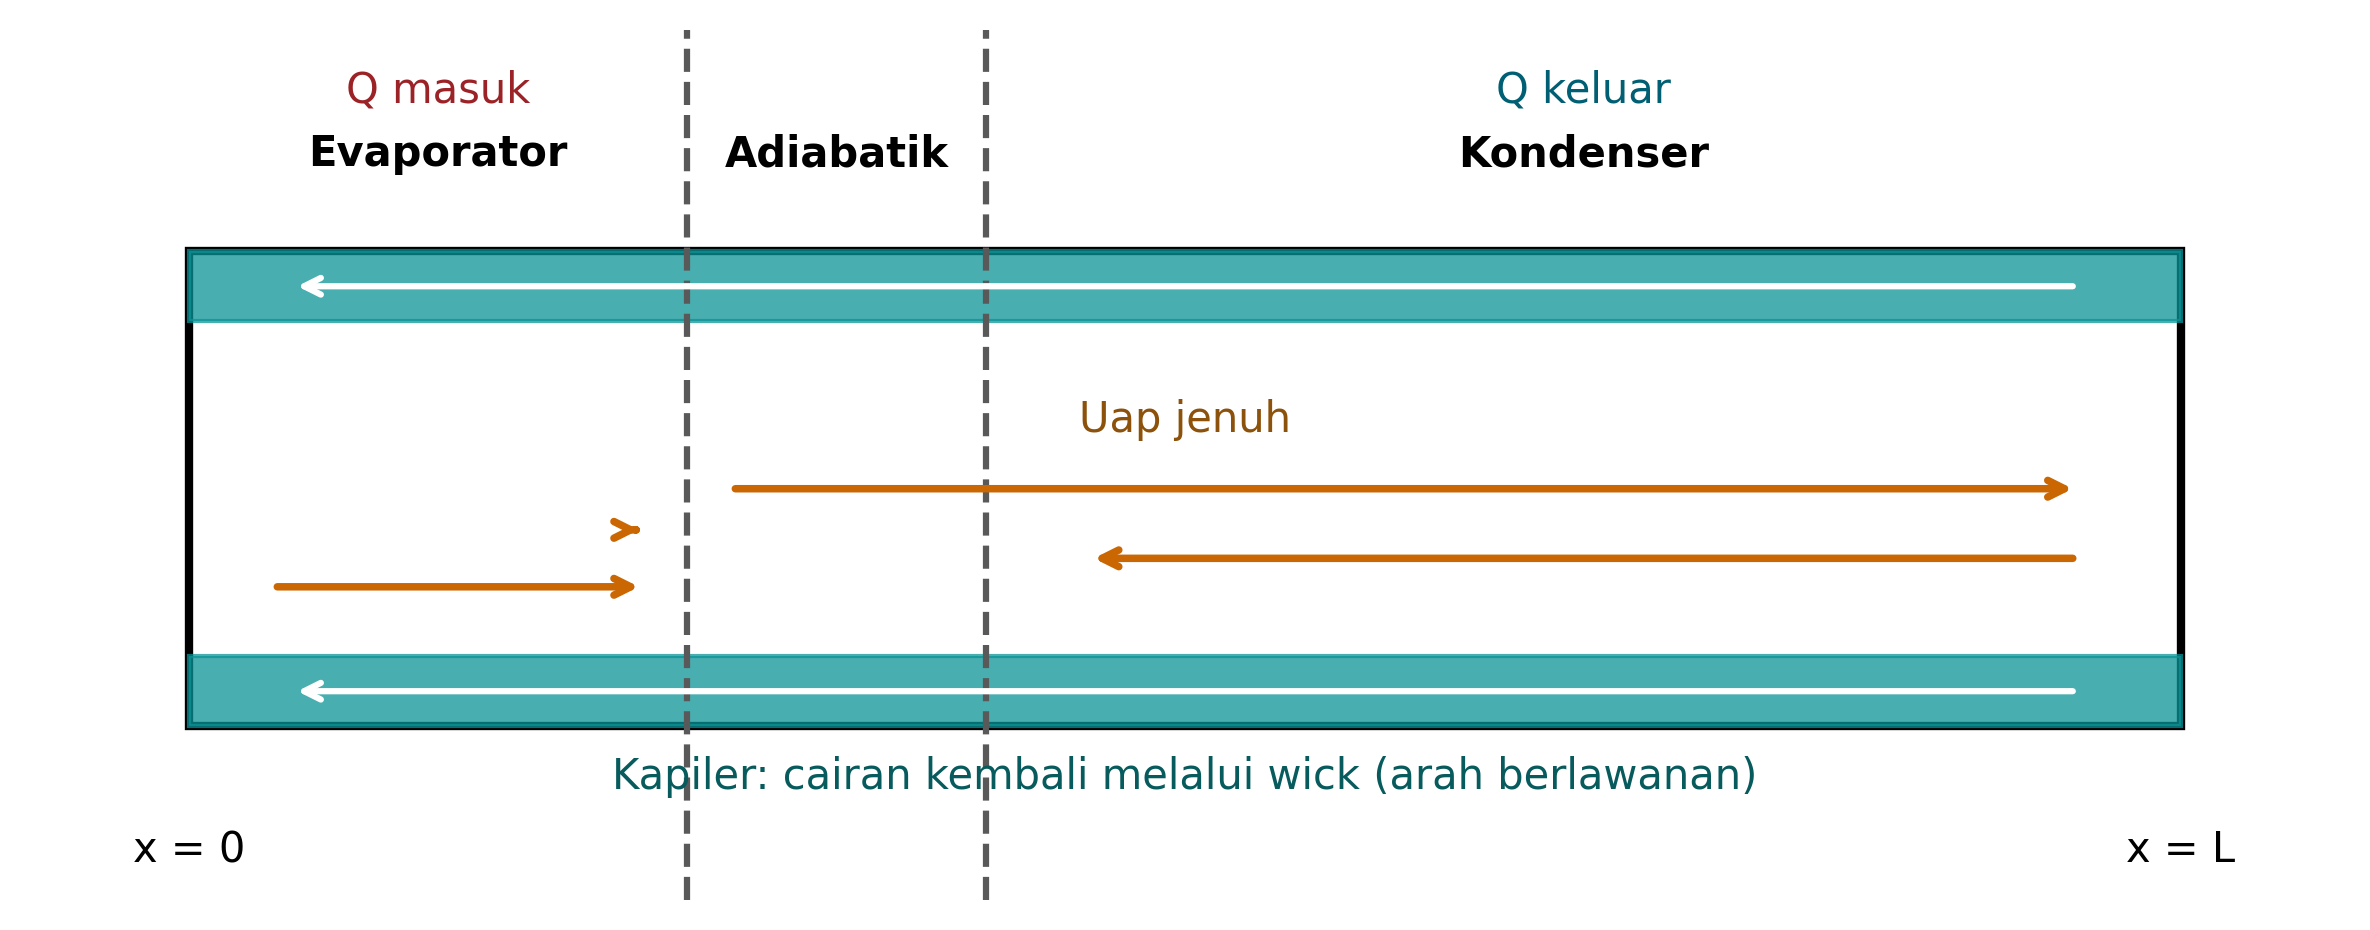
\includegraphics[width=0.95\textwidth,height=\textheight]{figures/skema-model.png}
\caption{Skema volume kontrol dan jalur aliran uap--cair yang digunakan
dalam model. Garis putus-putus menunjukkan batas evaporator, adiabatik,
dan kondenser.}\label{fig-skema}
}
\end{figure}

Asumsi kesetimbangan jenuh memungkinkan sifat cairan dan uap dievaluasi
pada temperatur operasi \(T_v\). Model tidak menyelesaikan distribusi
temperatur dinding atau antarmuka, sehingga \(T_v\) adalah temperatur
efektif untuk perhitungan hidraulik. Resistansi kondenser menghubungkan
temperatur tersebut dengan temperatur sink.

\hypertarget{neraca-energi-dan-massa}{%
\section{Neraca Energi dan Massa}\label{neraca-energi-dan-massa}}

Dengan kehilangan kalor pada bagian adiabatik diabaikan, daya yang masuk
evaporator sama dengan daya yang dilepas kondenser. Temperatur operasi
didekati dengan

\[
T_v=T_{sink}+R_cQ,
\tag{3.1}\]

dengan \(Q\) adalah daya masukan, \(R_c\) resistansi termal efektif
kondenser, dan \(T_{sink}\) temperatur sink. Pendekatan ini adalah
kondisi batas sederhana, bukan model radiator. Nilai \(R_c\) harus
diganti apabila radiasi atau pertukaran kalor diselesaikan secara lebih
rinci.

Laju aliran massa lokal berkaitan dengan kalor aksial \(Q_x(x)\) melalui
kalor laten:

\[
\dot m(x)=\frac{Q_x(x)}{h_{fg}}.
\tag{3.2}\]

Untuk pemanasan dan pendinginan merata, profil kalor aksial adalah

\[
Q_x(x)=
\begin{cases}
Q x/L_e, & 0\leq x\leq L_e,\\
Q, & L_e<x\leq L_e+L_a,\\
Q\left[1-(x-L_e-L_a)/L_c\right], & L_e+L_a<x\leq L.
\end{cases}
\tag{3.3}\]

Profil tersebut bernilai nol pada kedua ujung dan maksimum sebesar \(Q\)
di antara evaporator dan kondenser. Integral pembangkitan uap di
evaporator sama dengan integral kondensasi di kondenser sehingga neraca
massa global terpenuhi secara konstruksi.

\hypertarget{sifat-natrium}{%
\section{Sifat Natrium}\label{sifat-natrium}}

Tekanan jenuh natrium dihitung dengan korelasi Browning--Potter yang
direkomendasikan Fink dan Leibowitz {[}7{]}:

\[
\ln P=11{,}9463-\frac{12633{,}73}{T_v}-0{,}4672\ln T_v,
\tag{3.4}\]

dengan \(P\) dalam MPa dan \(T_v\) dalam K. Program mengonversi tekanan
ke Pa. Entalpi penguapan dihitung dengan

\[
h_{fg}=393{,}37(1-T_v/T_{cr})+4398{,}6(1-T_v/T_{cr})^{0{,}29302},
\tag{3.5}\]

dengan \(h_{fg}\) dalam kJ/kg dan \(T_{cr}=2503{,}7\) K. Densitas cairan
dalam kg/m³ adalah

\[
\rho_l=219+275{,}32\tau+511{,}58\tau^{1/2},
\qquad \tau=1-T_v/T_{cr}.
\tag{3.6}\]

Viskositas cairan dalam Pa·s dihitung dari

\[
\ln\mu_l=-6{,}4406-0{,}3958\ln T_v+\frac{556{,}835}{T_v}.
\tag{3.7}\]

Tegangan permukaan mengikuti bentuk Van der Waals:

\[
\sigma=0{,}2405(1-T_v/T_{cr})^{1{,}126}.
\tag{3.8}\]

Densitas uap didekati dengan gas ideal,

\[
\rho_v=\frac{PM}{R_uT_v},
\tag{3.9}\]

dengan massa molar natrium \(M=0{,}02298977\) kg/mol. Viskositas uap
menggunakan estimasi gas encer bola keras karena laporan sifat yang sama
tidak memberikan korelasi viskositas uap. Pendekatan ini merupakan
sumber ketidakpastian dan perlu diganti untuk analisis berketelitian
tinggi.

\hypertarget{aliran-uap}{%
\section{Aliran Uap}\label{aliran-uap}}

Kecepatan rata-rata uap pada setiap posisi adalah

\[
u_v(x)=\frac{\dot m(x)}{\rho_v A_v}.
\tag{3.10}\]

Bilangan Reynolds dan Mach dinyatakan sebagai

\[
Re_v=\frac{\rho_v u_vD_v}{\mu_v},\qquad Ma_v=\frac{u_v}{a_v},
\tag{3.11}\]

dengan \(a_v=\sqrt{\gamma R_vT_v}\) dan \(\gamma=5/3\) untuk pendekatan
gas monoatomik. Faktor gesek Darcy ditentukan dengan \(64/Re_v\) untuk
\(Re_v<2300\) dan korelasi Blasius \(0{,}3164Re_v^{-0{,}25}\) untuk
kondisi di luar rentang tersebut. Gradien rugi tekanan uap adalah

\[
\frac{d(\Delta P_v)}{dx}=\frac{f}{D_v}\frac{\rho_v u_v^2}{2}.
\tag{3.12}\]

Persamaan (3.12) diintegrasikan sepanjang pipa. Bilangan Mach digunakan
sebagai pemeriksaan penerimaan pendekatan tak kompresibel; kasus acuan
mensyaratkan \(Ma<0{,}3\). Apabila batas tersebut terlampaui, hasil
harus diinterpretasikan sebagai penyaringan dan model kompresibel
diperlukan.

\hypertarget{aliran-balik-cairan-dan-tekanan-kapiler}{%
\section{Aliran Balik Cairan dan Tekanan
Kapiler}\label{aliran-balik-cairan-dan-tekanan-kapiler}}

Aliran cairan di dalam medium berpori mengikuti hukum Darcy. Untuk arah
berlawanan dengan uap, besar gradien rugi tekanannya adalah

\[
\frac{d(\Delta P_l)}{dx}=\frac{\mu_l\dot m(x)}{\rho_l K A_w}.
\tag{3.13}\]

Untuk profil kalor pada Persamaan (3.3), integrasi menghasilkan panjang
efektif

\[
L_{eff}=\frac{L_e}{2}+L_a+\frac{L_c}{2}.
\tag{3.14}\]

Dengan demikian, rugi tekanan cairan total dapat pula ditulis dalam
bentuk kompak

\[
\Delta P_l=\frac{\mu_l Q L_{eff}}{\rho_l K A_w h_{fg}}.
\tag{3.15}\]

Tekanan kapiler maksimum didekati dengan persamaan Young--Laplace:

\[
\Delta P_{cap}=\frac{2\sigma\cos\theta_c}{r_c}.
\tag{3.16}\]

Kondisi operasi berkelanjutan adalah

\[
\Delta P_{cap}\geq \Delta P_v+\Delta P_l+\Delta P_g,
\tag{3.17}\]

dengan tekanan akibat percepatan efektif

\[
\Delta P_g=\rho_l g_{eff}L\sin\theta.
\tag{3.18}\]

Sudut \(\theta\) adalah kemiringan terhadap arah yang menghasilkan
komponen hidrostatik aksial. Pada kasus mikrogravitasi ideal,
\(g_{eff}=0\) sehingga \(\Delta P_g=0\). Model juga menerima percepatan
nonnol untuk meniru residu akselerasi atau membandingkan kondisi Bumi.
Nilai nol pada mikrogravitasi ideal tidak berarti seluruh masalah dua
fase menghilang; kapilaritas, gesekan, dan inersia uap tetap
diperhitungkan.

\hypertarget{batas-transportasi-kalor}{%
\section{Batas Transportasi Kalor}\label{batas-transportasi-kalor}}

Batas kapiler \(Q_{cap}\) adalah daya yang membuat ruas kanan Persamaan
(3.17) sama dengan \(\Delta P_{cap}\). Karena rugi tekanan uap tidak
selalu linear terhadap \(Q\), program mencari akar margin kapiler dengan
biseksi. Apabila tekanan hidrostatik saja sudah melebihi tekanan
kapiler, batas kapiler ditetapkan nol sebagai indikator ketidakmampuan
model beroperasi pada kondisi tersebut.

Batas sonik disaring menggunakan bentuk yang lazim dalam literatur pipa
kalor {[}3, 4{]}:

\[
Q_s=0{,}474 A_v h_{fg}\sqrt{\rho_vP}.
\tag{3.19}\]

Batas entrainment didekati dengan

\[
Q_{ent}=A_v h_{fg}\sqrt{\frac{\rho_v\sigma}{2r_c}}.
\tag{3.20}\]

Batas pendidihan di dalam sumbu dihitung sebagai

\[
Q_b=\frac{2\pi L_e k_{eff}T_v}{h_{fg}\rho_v\ln(r_i/r_v)}
\left(\frac{2\sigma}{r_b}-\Delta P_v-\Delta P_l-\Delta P_g\right),
\tag{3.21}\]

dengan \(k_{eff}\) konduktivitas efektif sumbu, \(r_b\) jari-jari
nukleasi, \(r_v\) jari-jari ruang uap, dan \(r_i=r_v+t_w\). Ketiga
persamaan terakhir bersifat penyaringan dengan ketidakpastian korelasi.
Nilai terkecil dari keempat batas digunakan sebagai batas pengatur untuk
perbandingan, tetapi bukan jaminan bahwa seluruh mekanisme kegagalan
telah tercakup.

\hypertarget{metode-numerik}{%
\section{Metode Numerik}\label{metode-numerik}}

Domain dibagi menjadi \(N\) sel dengan titik \(x_i=iL/N\). Besaran lokal
dihitung pada setiap titik. Integrasi rugi tekanan menggunakan aturan
trapesium:

\[
\int_0^L y(x)\,dx\approx\sum_{i=0}^{N-1}\frac{y_i+y_{i+1}}{2}(x_{i+1}-x_i).
\tag{3.22}\]

Untuk mencari \(Q_{cap}\), algoritme pertama memeriksa margin pada
\(Q=0\). Jika margin tidak positif, kapasitas kapiler adalah nol. Jika
positif, batas atas daya digandakan sampai margin berubah tanda. Biseksi
kemudian mempersempit interval. Skema ini dipilih karena margin menurun
secara monoton pada rentang yang dianalisis dan tidak membutuhkan
turunan.

\hypertarget{hipotesis}{%
\section{Hipotesis}\label{hipotesis}}

Berdasarkan persamaan di atas, dirumuskan dua dugaan yang diuji secara
numerik. Pertama, pada geometri acuan, rugi tekanan cairan lebih besar
daripada rugi tekanan uap sehingga batas kapiler menjadi pengatur pada
temperatur sekitar 1000 K. Kedua, peningkatan percepatan efektif pada
orientasi merugikan menurunkan kapasitas kapiler, sedangkan
mikrogravitasi ideal menghilangkan kontribusi hidrostatik. Dugaan ini
hanya berlaku untuk parameter yang diuji dan tidak digeneralisasi ke
seluruh desain pipa kalor.

\hypertarget{pelaksanaan-penelitian}{%
\chapter{PELAKSANAAN PENELITIAN}\label{pelaksanaan-penelitian}}

\hypertarget{alat-dan-bahan-penelitian}{%
\section{Alat dan Bahan Penelitian}\label{alat-dan-bahan-penelitian}}

Penelitian menggunakan perangkat lunak dan data sifat fluida; tidak
dilakukan eksperimen laboratorium. Simulator ditulis dalam Python 3.12.
NumPy 2.2.5 digunakan untuk larik dan operasi numerik, sedangkan
Matplotlib 3.10.3 digunakan untuk grafik {[}14, 15{]}. Pustaka standar
\texttt{dataclasses}, \texttt{csv}, \texttt{json}, \texttt{argparse},
dan \texttt{unittest} digunakan untuk struktur parameter, keluaran,
antarmuka perintah, dan pengujian. Dokumen disusun dalam format Quarto
Markdown dengan keluaran PDF berbasis LaTeX.

Struktur proyek dipisahkan menjadi sumber pada \texttt{src/}, pengujian
pada \texttt{tests/}, bab pada \texttt{chapters/}, lampiran pada
\texttt{appendices/}, data pada \texttt{data/}, dan gambar pada
\texttt{figures/}. Pemisahan tersebut mencegah pencampuran antara
persamaan, keluaran numerik, dan naskah. Nama berkas keluaran
menggunakan bahasa Indonesia agar mudah dikenali dalam pembahasan.

Parameter geometri dan kondisi acuan diberikan pada Tabel IV.1. Geometri
bukan salinan pipa kalor reaktor tertentu, melainkan kasus representatif
yang dipilih agar model memperlihatkan mekanisme kapiler, uap, dan
gravitasi dalam satu rangkaian perhitungan.

\begin{longtable}[]{@{}lcrc@{}}
\caption{Parameter geometri, sumbu, dan kondisi batas kasus
acuan.}\tabularnewline
\toprule
Parameter & Simbol & Nilai & Satuan \\
\midrule
\endfirsthead
\toprule
Parameter & Simbol & Nilai & Satuan \\
\midrule
\endhead
Panjang evaporator & \(L_e\) & 0,25 & m \\
Panjang adiabatik & \(L_a\) & 0,15 & m \\
Panjang kondenser & \(L_c\) & 0,60 & m \\
Diameter ruang uap & \(D_v\) & 0,012 & m \\
Tebal sumbu & \(t_w\) & 0,001 & m \\
Jari-jari pori efektif & \(r_c\) & 75 & µm \\
Permeabilitas & \(K\) & \(5\times10^{-10}\) & m² \\
Sudut kontak & \(\theta_c\) & 0 & ° \\
Konduktivitas efektif sumbu & \(k_{eff}\) & 10 & W/(m·K) \\
Jari-jari nukleasi & \(r_b\) & 5 & µm \\
Daya masukan & \(Q\) & 800 & W \\
Temperatur sink & \(T_{sink}\) & 700 & K \\
Resistansi kondenser & \(R_c\) & 0,375 & K/W \\
Percepatan efektif & \(g_{eff}\) & 0 & m/s² \\
Jumlah sel & \(N\) & 400 & -- \\
\bottomrule
\end{longtable}

Nilai turunan yang digunakan adalah panjang total 1,00 m, panjang
efektif 0,575 m, luas ruang uap \(1{,}13097\times10^{-4}\) m², dan luas
sumbu \(4{,}08407\times10^{-5}\) m². Sifat natrium dihitung pada setiap
temperatur operasi, bukan diambil sebagai konstanta.

\hypertarget{tata-laksana-penelitian}{%
\section{Tata Laksana Penelitian}\label{tata-laksana-penelitian}}

Tahapan penelitian dilaksanakan sebagai berikut.

\begin{enumerate}
\def\labelenumi{\arabic{enumi}.}
\tightlist
\item
  Menurunkan neraca energi, profil kalor aksial, laju aliran massa, rugi
  tekanan uap, rugi tekanan cairan, dan neraca kapiler.
\item
  Mengimplementasikan korelasi sifat natrium pada kelas
  \texttt{SodiumProperties} dengan pemeriksaan rentang temperatur.
\item
  Menyusun parameter pada kelas data \texttt{HeatPipeGeometry} dan
  \texttt{OperatingConditions} agar masukan dapat divalidasi dan diubah
  tanpa mengedit persamaan.
\item
  Membentuk profil kalor aksial sesuai Persamaan (3.3) dan menghitung
  kecepatan, Reynolds, serta Mach.
\item
  Mengintegrasikan rugi tekanan dengan aturan trapesium dan mengevaluasi
  margin kapiler.
\item
  Menghitung batas sonik, entrainment, dan pendidihan pada temperatur
  operasi.
\item
  Mencari batas kapiler melalui bracketing dan biseksi pada temperatur
  tetap.
\item
  Menjalankan kasus acuan, peta batas pada 800--1200 K, studi beban,
  studi percepatan, studi pori, dan konvergensi grid.
\item
  Menyimpan data dalam CSV/JSON dan membuat gambar langsung dari hasil
  perhitungan.
\item
  Menjalankan pengujian otomatis dan memeriksa konsistensi antara angka
  dalam naskah dan berkas keluaran.
\end{enumerate}

Perintah reproduksi dari direktori utama proyek adalah sebagai berikut.

\begin{Shaded}
\begin{Highlighting}[]
\ExtensionTok{python} \AttributeTok{{-}m}\NormalTok{ pip install }\AttributeTok{{-}r}\NormalTok{ requirements.txt}
\ExtensionTok{python}\NormalTok{ src/heatpipe\_simulator.py}
\ExtensionTok{python} \AttributeTok{{-}m}\NormalTok{ unittest discover }\AttributeTok{{-}s}\NormalTok{ tests }\AttributeTok{{-}v}
\ExtensionTok{quarto}\NormalTok{ render Skripsi.qmd }\AttributeTok{{-}{-}to}\NormalTok{ pdf}
\end{Highlighting}
\end{Shaded}

Program tidak membutuhkan koneksi internet pada saat simulasi. Instalasi
paket dan renderer hanya diperlukan pada penyiapan awal. Seluruh
keluaran menggunakan satuan SI secara internal; pemformatan desimal pada
naskah dilakukan ketika hasil disajikan.

\hypertarget{rencana-analisis-hasil-penelitian}{%
\section{Rencana Analisis Hasil
Penelitian}\label{rencana-analisis-hasil-penelitian}}

Hasil utama dirangkum dalam enam kelompok. Pertama, sifat fluida pada
1000 K diperiksa terhadap nilai acuan. Kedua, kasus acuan dianalisis
melalui laju massa maksimum, kecepatan, Reynolds, Mach, rugi tekanan,
margin kapiler, dan empat batas operasi. Ketiga, peta batas terhadap
temperatur digunakan untuk mengidentifikasi mekanisme pengatur.

Keempat, studi beban dilakukan dengan mempertahankan \(T_{sink}\) dan
\(R_c\), sehingga temperatur operasi berubah mengikuti Persamaan (3.1).
Analisis ini tidak sama dengan peta pada temperatur tetap. Kelima, studi
percepatan dilakukan pada 1000 K untuk \(g_{eff}=0\), 0,01, 0,1, 1, dan
9,81 m/s². Orientasi 90° digunakan untuk kasus nonnol agar seluruh
komponen aksial bekerja merugikan. Keenam, jari-jari pori divariasikan
dengan permeabilitas tetap untuk mengisolasi pengaruh tekanan kapiler
dan entrainment.

Konvergensi grid dinilai dari jumlah rugi tekanan uap dan cairan pada
\(N=50\) sampai 1600. Grid 1600 digunakan sebagai pembanding relatif.
Karena profil kalor aksial merupakan fungsi linear per bagian, integrasi
trapesium diperkirakan menjadi sangat tepat ketika batas bagian berimpit
dengan titik grid.

Verifikasi program dilakukan melalui sepuluh pengujian yang tercantum
pada Tabel IV.2. Pengujian ini memeriksa implementasi dan konsistensi
fisik, tetapi tidak menggantikan validasi eksperimental.

\begin{longtable}[]{@{}
  >{\raggedright\arraybackslash}p{(\columnwidth - 4\tabcolsep) * \real{0.2778}}
  >{\raggedright\arraybackslash}p{(\columnwidth - 4\tabcolsep) * \real{0.4444}}
  >{\raggedright\arraybackslash}p{(\columnwidth - 4\tabcolsep) * \real{0.2778}}@{}}
\caption{Rancangan verifikasi perangkat lunak.}\tabularnewline
\toprule
\begin{minipage}[b]{\linewidth}\raggedright
Kelompok
\end{minipage} & \begin{minipage}[b]{\linewidth}\raggedright
Hal yang diuji
\end{minipage} & \begin{minipage}[b]{\linewidth}\raggedright
Kriteria
\end{minipage} \\
\midrule
\endfirsthead
\toprule
\begin{minipage}[b]{\linewidth}\raggedright
Kelompok
\end{minipage} & \begin{minipage}[b]{\linewidth}\raggedright
Hal yang diuji
\end{minipage} & \begin{minipage}[b]{\linewidth}\raggedright
Kriteria
\end{minipage} \\
\midrule
\endhead
Sifat fluida & Tekanan jenuh pada titik didih normal & Sekitar 1 atm
pada 1156 K \\
Sifat fluida & \(\sigma\), \(\mu_l\), \(h_{fg}\), dan \(\rho_l\) pada
1000 K & Sesuai nilai acuan/toleransi \\
Sifat fluida & Semua sifat pada 1000 K & Positif dan berhingga \\
Profil energi & Nilai ujung, maksimum, dan arah gradien &
Nol--maksimum--nol sesuai geometri \\
Mikrogravitasi & Tekanan hidrostatik & Nol ketika \(g_{eff}=0\) \\
Kasus acuan & Mekanisme pengatur dan Mach & Kapiler dan \(Ma<0,3\) \\
Batas kapiler & Margin pada \(Q=Q_{cap}\) & Mendekati nol \\
Percepatan & Kapasitas pada orientasi merugikan & Menurun; kasus Bumi
acuan tidak feasible \\
Grid & Rugi tekanan grid 100 dan 1600 & Selisih relatif
\textless0,5\% \\
Validasi masukan & Permeabilitas nol & Ditolak oleh program \\
\bottomrule
\end{longtable}

\hypertarget{hasil-dan-pembahasan}{%
\chapter{HASIL DAN PEMBAHASAN}\label{hasil-dan-pembahasan}}

\hypertarget{hasil-kasus-acuan}{%
\section{Hasil Kasus Acuan}\label{hasil-kasus-acuan}}

Kasus acuan menghasilkan temperatur operasi 1000 K dari hubungan
\(T_v=700+0{,}375(800)\). Sifat fluida yang digunakan pada temperatur
tersebut disajikan pada Tabel V.1. Tekanan jenuh sebesar 19,95 kPa dan
kalor laten sekitar 4,02 MJ/kg menghasilkan laju aliran massa maksimum
\(1{,}98784\times10^{-4}\) kg/s.

\begin{longtable}[]{@{}lrc@{}}
\caption{Sifat natrium pada temperatur operasi 1000 K.}\tabularnewline
\toprule
Besaran & Nilai & Satuan \\
\midrule
\endfirsthead
\toprule
Besaran & Nilai & Satuan \\
\midrule
\endhead
Tekanan jenuh & 19.945,87 & Pa \\
Kalor laten & 4.024.461,18 & J/kg \\
Densitas cairan & 780,818 & kg/m³ \\
Densitas uap & 0,055151 & kg/m³ \\
Viskositas cairan & \(1{,}80848\times10^{-4}\) & Pa·s \\
Viskositas uap & \(2{,}52981\times10^{-5}\) & Pa·s \\
Tegangan permukaan & 0,135455 & N/m \\
Konduktivitas cairan & 54,244 & W/(m·K) \\
Kecepatan suara pendekatan & 776,380 & m/s \\
\bottomrule
\end{longtable}

Hasil hidraulik utama diberikan pada Tabel V.2. Rugi tekanan cairan
sebesar 1296,43 Pa jauh lebih besar daripada rugi tekanan uap sebesar
103,02 Pa. Perbandingan ini konsisten dengan dominasi hambatan viskos
pada kanal berpori. Tekanan kapiler yang tersedia adalah 3612,13 Pa
sehingga tersisa margin 2212,68 Pa. Tidak ada tekanan hidrostatik karena
percepatan efektif ditetapkan nol.

\begin{longtable}[]{@{}lr@{}}
\caption{Ringkasan hasil kasus acuan 800 W pada
mikrogravitasi.}\tabularnewline
\toprule
Besaran & Nilai \\
\midrule
\endfirsthead
\toprule
Besaran & Nilai \\
\midrule
\endhead
Laju massa maksimum & \(1{,}98784\times10^{-4}\) kg/s \\
Kecepatan uap maksimum & 31,8696 m/s \\
Bilangan Reynolds maksimum & 833,724 \\
Bilangan Mach maksimum & 0,04105 \\
Tekanan kapiler & 3612,13 Pa \\
Rugi tekanan uap & 103,02 Pa \\
Rugi tekanan cairan & 1296,43 Pa \\
Rugi tekanan gravitasi & 0 Pa \\
Margin kapiler & 2212,68 Pa \\
Utilisasi batas pengatur & 38,74\% \\
\bottomrule
\end{longtable}

Bilangan Reynolds maksimum berada dalam rentang laminar pada model dan
bilangan Mach jauh di bawah 0,3. Oleh karena itu, penggunaan pendekatan
rugi tekanan tak kompresibel dapat diterima untuk kasus ini sebagai
penyaringan. Pernyataan tersebut tidak berlaku otomatis pada temperatur
rendah ketika densitas uap jauh lebih kecil.

\hypertarget{profil-aksial}{%
\section{Profil Aksial}\label{profil-aksial}}

Gambar V.1 menunjukkan kalor aksial meningkat linear di evaporator,
konstan pada bagian adiabatik, lalu menurun linear di kondenser.
Kecepatan uap mengikuti bentuk yang sama karena sifat fluida dan luas
penampang konstan pada satu perhitungan. Nilai maksimum terjadi di
sepanjang bagian adiabatik, yaitu antara \(x=0,25\) m dan \(x=0,40\) m.

\begin{figure}
\hypertarget{fig-profil}{%
\centering
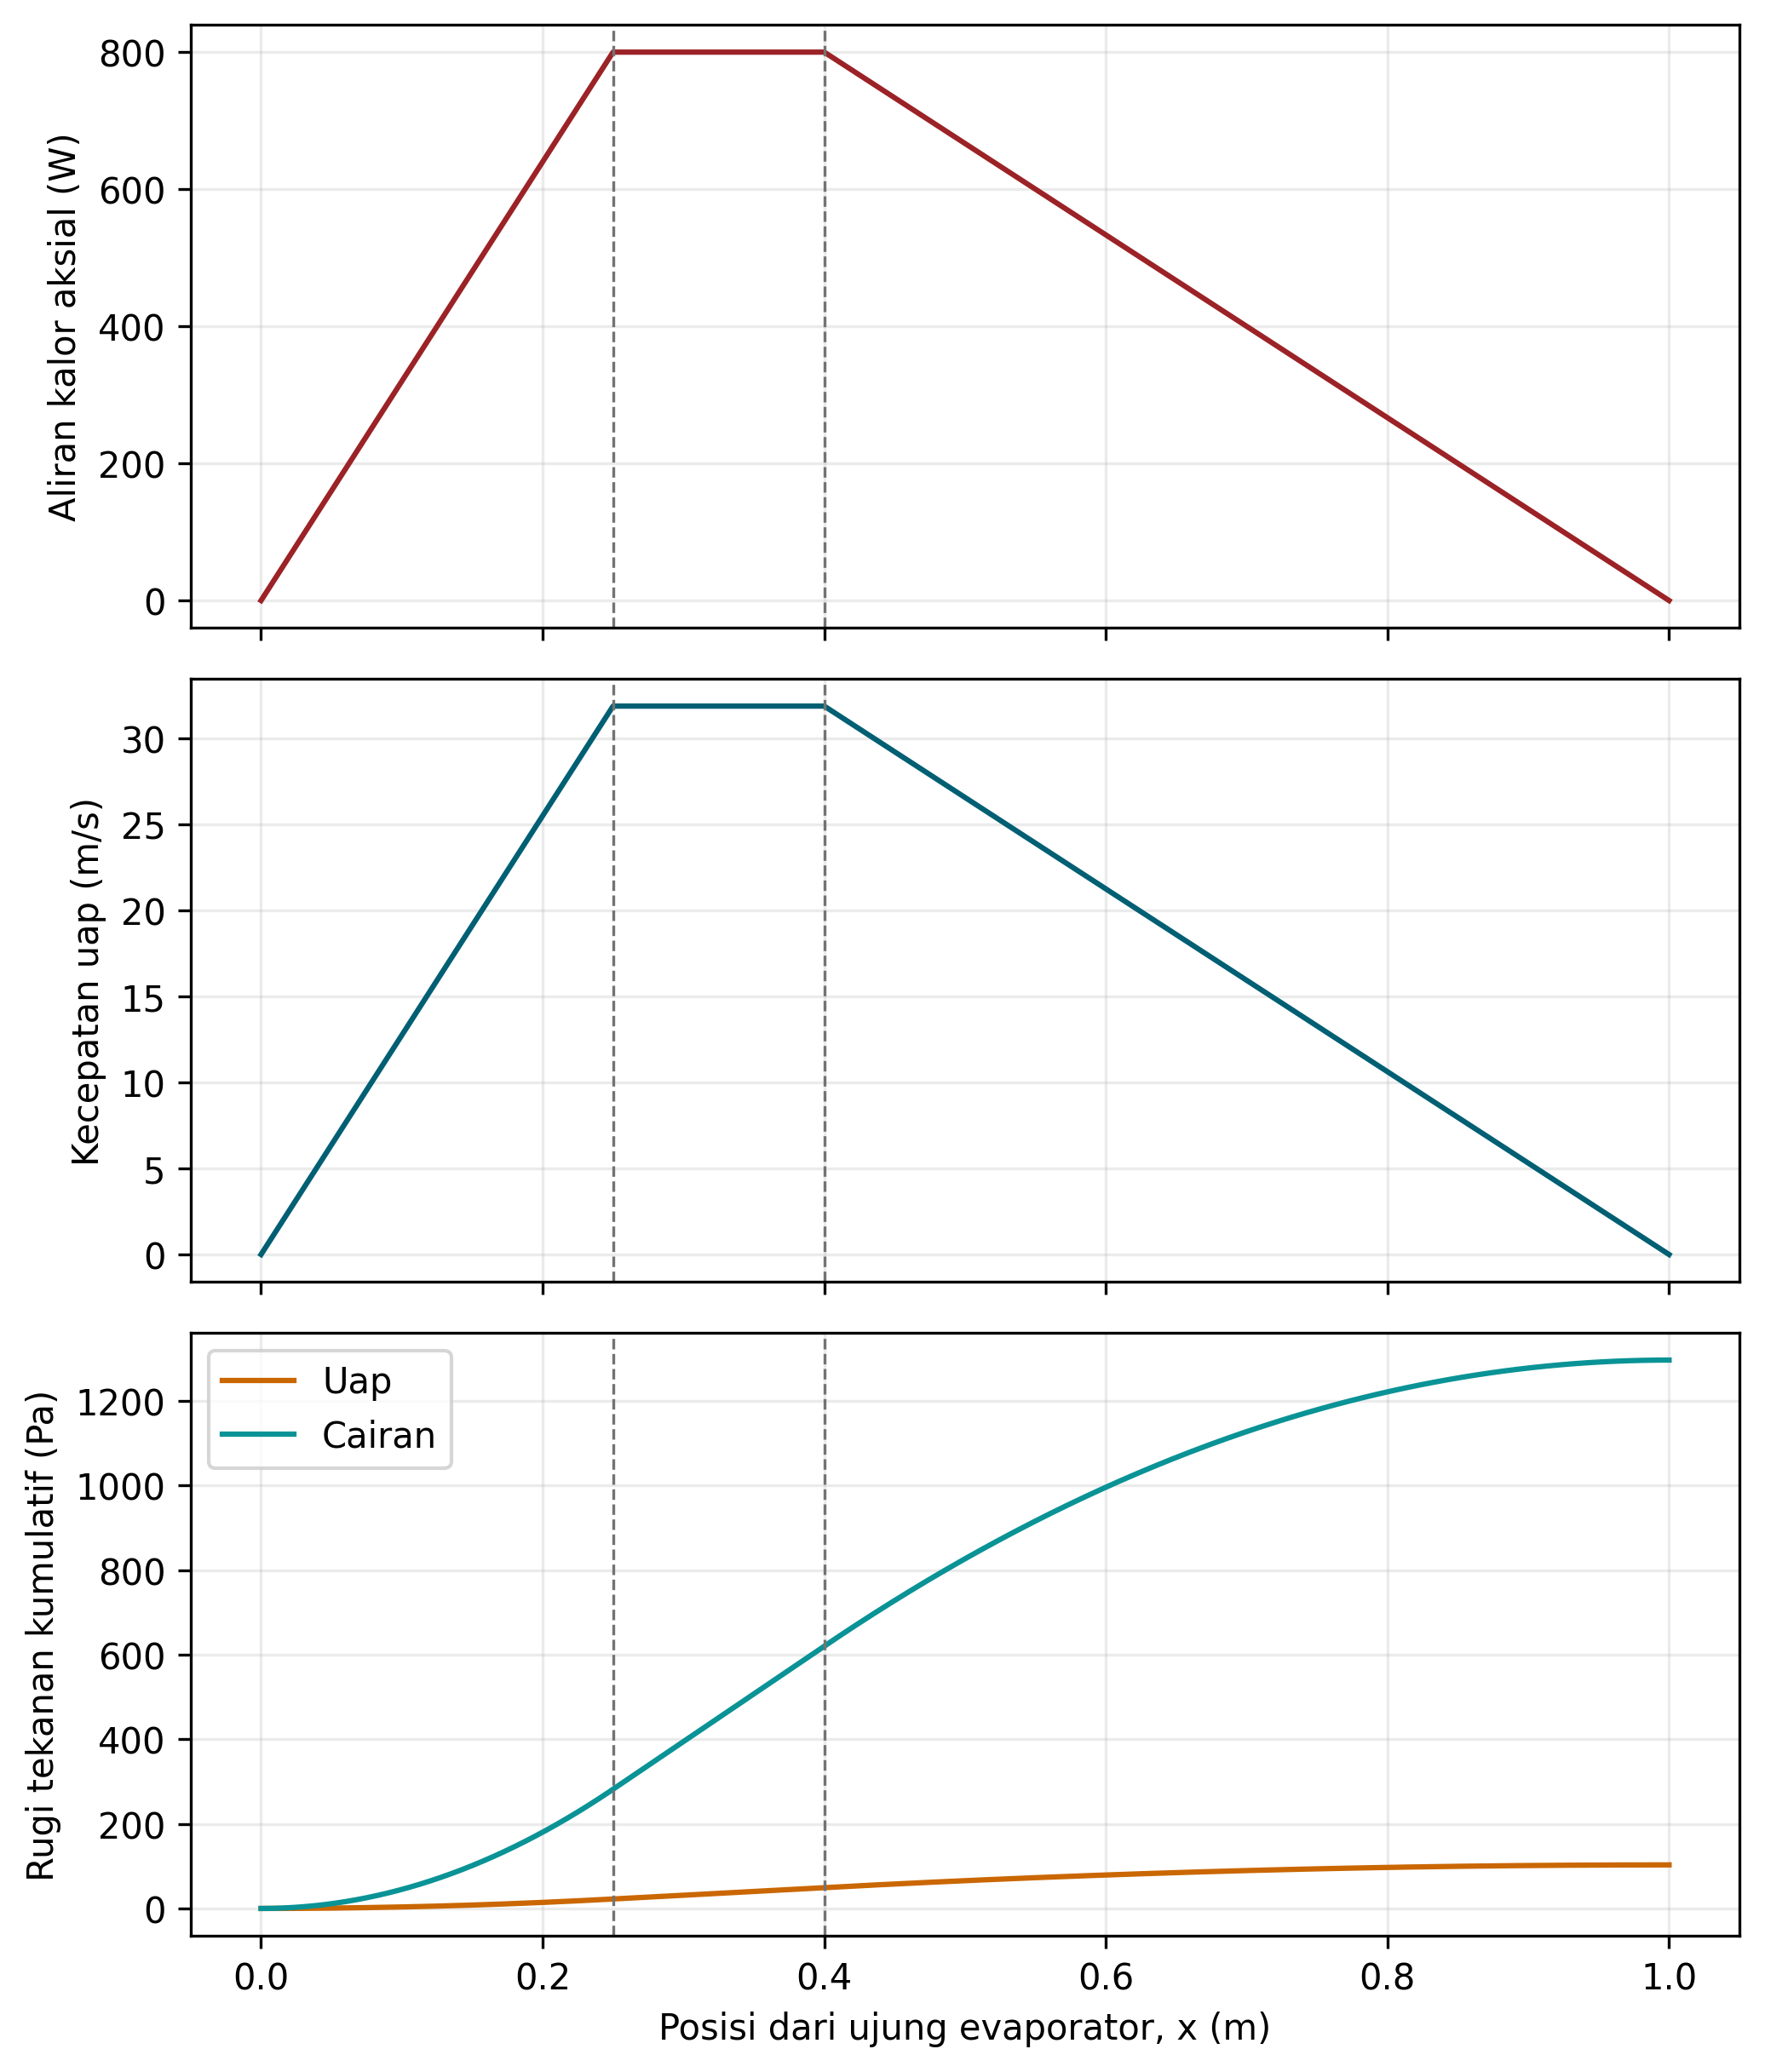
\includegraphics[width=0.88\textwidth,height=\textheight]{figures/profil-aksial.png}
\caption{Profil kalor aksial, kecepatan uap, dan rugi tekanan kumulatif
untuk kasus acuan. Posisi \(x=0\) adalah ujung evaporator; garis batas
berada pada 0,25 m dan 0,40 m.}\label{fig-profil}
}
\end{figure}

Rugi tekanan kumulatif bertambah paling cepat di bagian adiabatik karena
laju massa berada pada nilai maksimum. Di evaporator dan kondenser,
gradien berubah mengikuti profil laju massa. Rugi tekanan cairan
memiliki bentuk serupa dengan skala yang lebih besar. Hasil ini
menegaskan bahwa panjang efektif dalam Persamaan (3.14) bukan sekadar
panjang total; distribusi pemanasan dan pendinginan ikut menentukan
integrasi aliran.

\hypertarget{batas-operasi-dan-pengaruh-temperatur}{%
\section{Batas Operasi dan Pengaruh
Temperatur}\label{batas-operasi-dan-pengaruh-temperatur}}

Pada kasus acuan, batas kapiler adalah 2064,88 W, batas sonik 7155,53 W,
batas entrainment 3212,10 W, dan batas pendidihan 24.232,80 W. Batas
kapiler merupakan nilai terkecil sehingga menjadi pengatur. Daya 800 W
menggunakan 38,74\% dari batas tersebut. Batas pendidihan bergantung
pada rugi tekanan kasus aktual, sedangkan peta temperatur menggunakan
proba daya kecil agar perbandingan sifat lebih konsisten; karena itu
terdapat perbedaan kecil antara nilai pendidihan pada peta dan kasus
acuan.

Tabel V.3 dan Gambar V.2 memperlihatkan perubahan mekanisme pengatur.
Pada 800 K batas sonik hanya 393,48 W, lebih rendah daripada batas
kapiler dan entrainment. Pada 900 K, batas entrainment sedikit lebih
rendah daripada batas kapiler. Pada 1000--1200 K, batas kapiler menjadi
pengatur. Peningkatan temperatur menaikkan tekanan dan densitas uap
sehingga batas sonik meningkat tajam. Sebaliknya, tegangan permukaan
menurun terhadap temperatur dan pada akhirnya mengurangi tekanan
kapiler.

\begin{small}

\begin{longtable}[]{@{}
  >{\raggedleft\arraybackslash}p{(\columnwidth - 10\tabcolsep) * \real{0.1928}}
  >{\raggedleft\arraybackslash}p{(\columnwidth - 10\tabcolsep) * \real{0.1566}}
  >{\raggedleft\arraybackslash}p{(\columnwidth - 10\tabcolsep) * \real{0.1325}}
  >{\raggedleft\arraybackslash}p{(\columnwidth - 10\tabcolsep) * \real{0.2048}}
  >{\raggedleft\arraybackslash}p{(\columnwidth - 10\tabcolsep) * \real{0.1928}}
  >{\raggedright\arraybackslash}p{(\columnwidth - 10\tabcolsep) * \real{0.1205}}@{}}
\caption{Peta batas transportasi kalor pada temperatur
tetap.}\tabularnewline
\toprule
\begin{minipage}[b]{\linewidth}\raggedleft
Temperatur (K)
\end{minipage} & \begin{minipage}[b]{\linewidth}\raggedleft
Kapiler (W)
\end{minipage} & \begin{minipage}[b]{\linewidth}\raggedleft
Sonik (W)
\end{minipage} & \begin{minipage}[b]{\linewidth}\raggedleft
Entrainment (W)
\end{minipage} & \begin{minipage}[b]{\linewidth}\raggedleft
Pendidihan (W)
\end{minipage} & \begin{minipage}[b]{\linewidth}\raggedright
Pengatur
\end{minipage} \\
\midrule
\endfirsthead
\toprule
\begin{minipage}[b]{\linewidth}\raggedleft
Temperatur (K)
\end{minipage} & \begin{minipage}[b]{\linewidth}\raggedleft
Kapiler (W)
\end{minipage} & \begin{minipage}[b]{\linewidth}\raggedleft
Sonik (W)
\end{minipage} & \begin{minipage}[b]{\linewidth}\raggedleft
Entrainment (W)
\end{minipage} & \begin{minipage}[b]{\linewidth}\raggedleft
Pendidihan (W)
\end{minipage} & \begin{minipage}[b]{\linewidth}\raggedright
Pengatur
\end{minipage} \\
\midrule
\endhead
800 & 1119,89 & 393,48 & 872,58 & 372.531,62 & Sonik \\
900 & 1828,89 & 1989,01 & 1822,46 & 82.149,60 & Entrainment \\
1000 & 2064,88 & 7155,53 & 3212,10 & 24.874,49 & Kapiler \\
1100 & 2066,85 & 20.110,97 & 5000,63 & 9449,29 & Kapiler \\
1200 & 1969,78 & 46.978,71 & 7086,28 & 4241,04 & Kapiler \\
\bottomrule
\end{longtable}

\end{small}

\begin{figure}
\hypertarget{fig-batas}{%
\centering
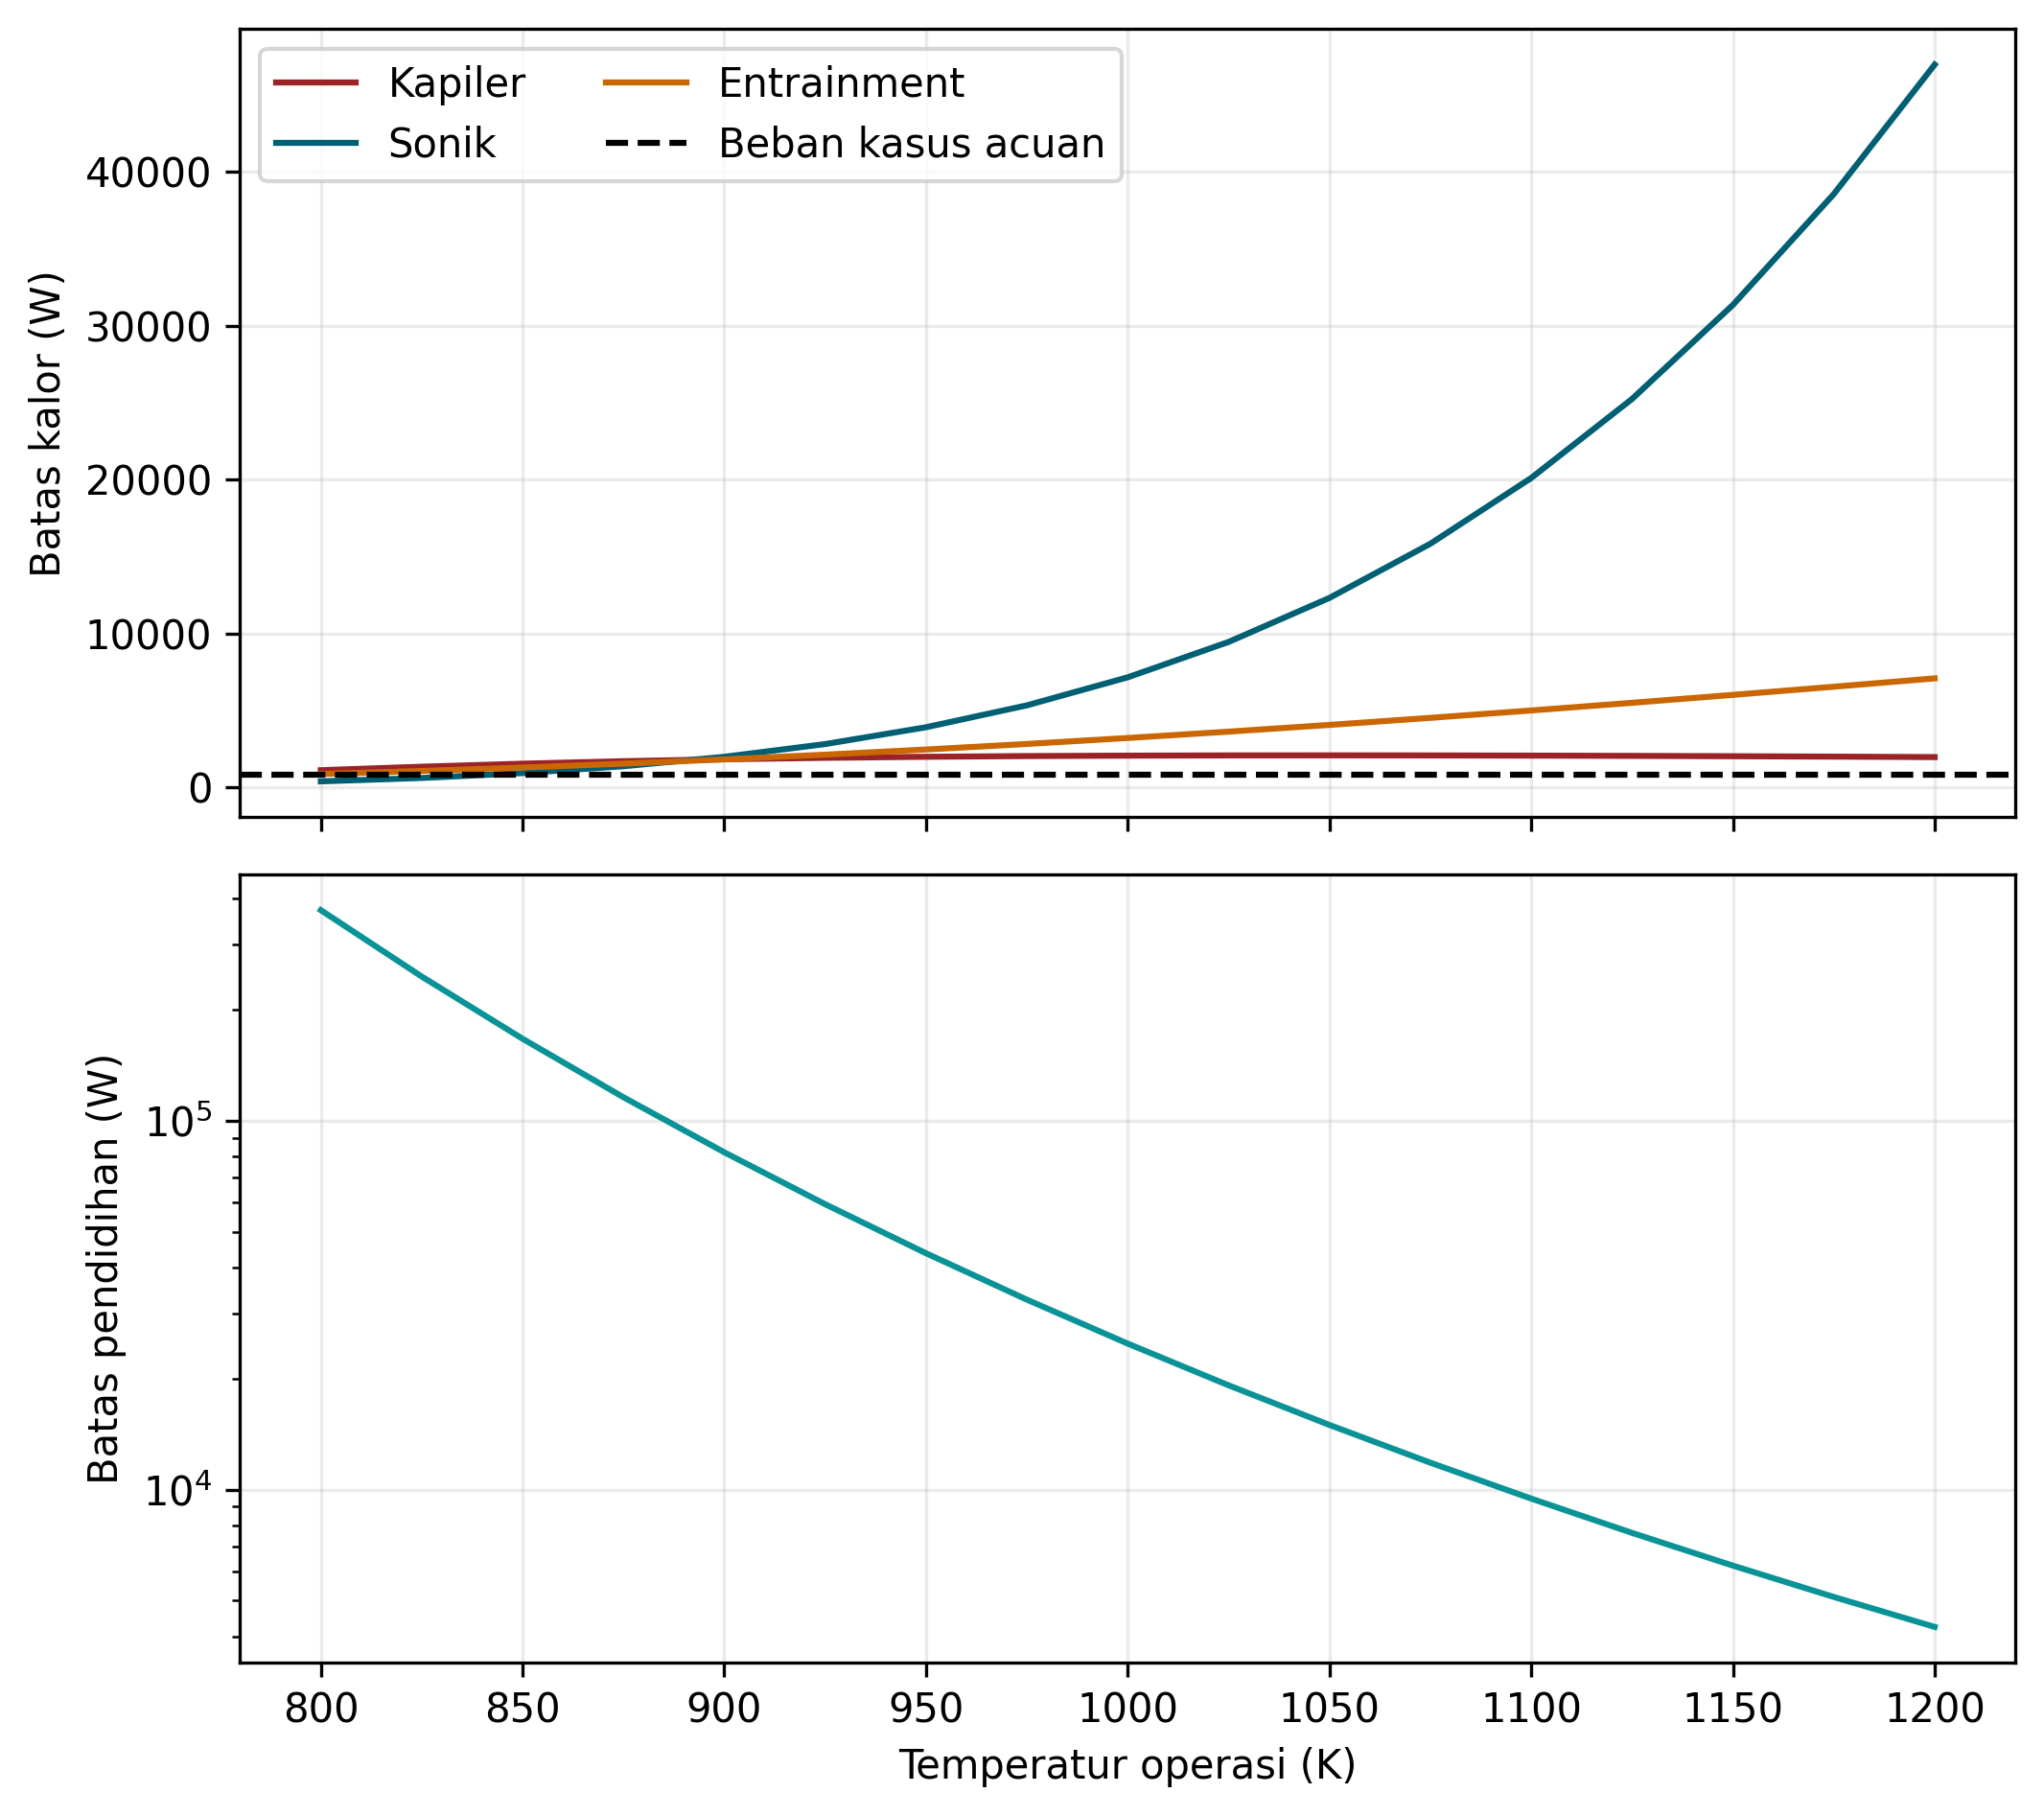
\includegraphics[width=0.92\textwidth,height=\textheight]{figures/batas-operasi.png}
\caption{Peta batas operasi terhadap temperatur. Panel atas menampilkan
batas kapiler, sonik, entrainment, dan beban acuan; panel bawah
menampilkan batas pendidihan dalam skala logaritmik.}\label{fig-batas}
}
\end{figure}

Batas kapiler meningkat dari 800 K hingga sekitar 1050--1100 K kemudian
menurun. Perilaku nonmonoton tersebut muncul dari kompetisi beberapa
sifat: kenaikan kalor laten atau densitas uap memengaruhi rugi tekanan
dan laju massa, sedangkan viskositas cairan serta tegangan permukaan
menurun. Model tidak mendukung kesimpulan bahwa temperatur yang lebih
tinggi selalu meningkatkan kapasitas. Selain itu, hasil di bawah rentang
rekomendasi sifat atau di dekat kondisi sonik harus diperlakukan dengan
kehati-hatian.

\hypertarget{pengaruh-beban-kalor}{%
\section{Pengaruh Beban Kalor}\label{pengaruh-beban-kalor}}

Studi beban menggunakan resistansi kondenser tetap sehingga setiap
kenaikan daya juga menaikkan temperatur operasi. Hasil pada Tabel V.4
memperlihatkan dua pengaruh yang berlawanan. Kenaikan daya meningkatkan
laju massa yang diperlukan, tetapi kenaikan temperatur meningkatkan
densitas uap dan dapat menurunkan kecepatan serta Mach. Akibatnya, Mach
maksimum justru menurun dari 0,223 pada 300 W menjadi 0,00617 pada 1600
W. Perilaku ini merupakan konsekuensi kondisi batas
\(T_v=T_{sink}+R_cQ\), bukan karakter universal pipa kalor.

\begin{small}

\begin{longtable}[]{@{}
  >{\raggedleft\arraybackslash}p{(\columnwidth - 10\tabcolsep) * \real{0.1149}}
  >{\raggedleft\arraybackslash}p{(\columnwidth - 10\tabcolsep) * \real{0.1839}}
  >{\raggedright\arraybackslash}p{(\columnwidth - 10\tabcolsep) * \real{0.1149}}
  >{\raggedleft\arraybackslash}p{(\columnwidth - 10\tabcolsep) * \real{0.1724}}
  >{\raggedleft\arraybackslash}p{(\columnwidth - 10\tabcolsep) * \real{0.1724}}
  >{\raggedleft\arraybackslash}p{(\columnwidth - 10\tabcolsep) * \real{0.2414}}@{}}
\caption{Studi beban dengan temperatur sink dan resistansi kondenser
tetap.}\tabularnewline
\toprule
\begin{minipage}[b]{\linewidth}\raggedleft
Daya (W)
\end{minipage} & \begin{minipage}[b]{\linewidth}\raggedleft
Temperatur (K)
\end{minipage} & \begin{minipage}[b]{\linewidth}\raggedright
Pengatur
\end{minipage} & \begin{minipage}[b]{\linewidth}\raggedleft
Utilisasi (\%)
\end{minipage} & \begin{minipage}[b]{\linewidth}\raggedleft
Mach maksimum
\end{minipage} & \begin{minipage}[b]{\linewidth}\raggedleft
Margin kapiler (Pa)
\end{minipage} \\
\midrule
\endfirsthead
\toprule
\begin{minipage}[b]{\linewidth}\raggedleft
Daya (W)
\end{minipage} & \begin{minipage}[b]{\linewidth}\raggedleft
Temperatur (K)
\end{minipage} & \begin{minipage}[b]{\linewidth}\raggedright
Pengatur
\end{minipage} & \begin{minipage}[b]{\linewidth}\raggedleft
Utilisasi (\%)
\end{minipage} & \begin{minipage}[b]{\linewidth}\raggedleft
Mach maksimum
\end{minipage} & \begin{minipage}[b]{\linewidth}\raggedleft
Margin kapiler (Pa)
\end{minipage} \\
\midrule
\endhead
300 & 812,5 & Sonik & 60,85 & 0,22343 & 3121,80 \\
600 & 925,0 & Kapiler & 31,20 & 0,07824 & 2625,15 \\
800 & 1000,0 & Kapiler & 38,74 & 0,04105 & 2212,68 \\
1200 & 1150,0 & Kapiler & 59,21 & 0,01405 & 1308,82 \\
1600 & 1300,0 & Kapiler & 87,75 & 0,00617 & 344,51 \\
\bottomrule
\end{longtable}

\end{small}

Margin kapiler menurun ketika beban menjadi besar dan utilisasi mencapai
87,75\% pada 1600 W. Oleh sebab itu, peningkatan beban tetap mendekatkan
sistem pada keterbatasan meskipun Mach menurun. Hasil ini memperlihatkan
bahwa pemeriksaan satu indikator tidak cukup untuk menilai kelayakan
operasi.

\hypertarget{pengaruh-percepatan-efektif}{%
\section{Pengaruh Percepatan
Efektif}\label{pengaruh-percepatan-efektif}}

Gambar V.3 dan Tabel V.5 menunjukkan batas kapiler pada 1000 K untuk
beberapa percepatan. Percepatan 0,01 m/s² pada orientasi 90° hanya
menurunkan kapasitas dari 2064,88 W menjadi 2060,42 W. Penurunan menjadi
lebih besar pada 1 m/s², yaitu 1618,53 W. Pada percepatan 9,81 m/s²
dengan orientasi merugikan, tekanan hidrostatik melebihi tekanan kapiler
sehingga tidak ada kapasitas positif menurut model.

\begin{longtable}[]{@{}rcr@{}}
\caption{Pengaruh percepatan efektif pada batas kapiler pada 1000
K.}\tabularnewline
\toprule
Percepatan (m/s²) & Orientasi & Batas kapiler (W) \\
\midrule
\endfirsthead
\toprule
Percepatan (m/s²) & Orientasi & Batas kapiler (W) \\
\midrule
\endhead
0 & 0° & 2064,88 \\
0,01 & 90° & 2060,42 \\
0,1 & 90° & 2020,25 \\
1 & 90° & 1618,53 \\
9,81 & 90° & 0 \\
\bottomrule
\end{longtable}

\begin{figure}
\hypertarget{fig-gravitasi}{%
\centering
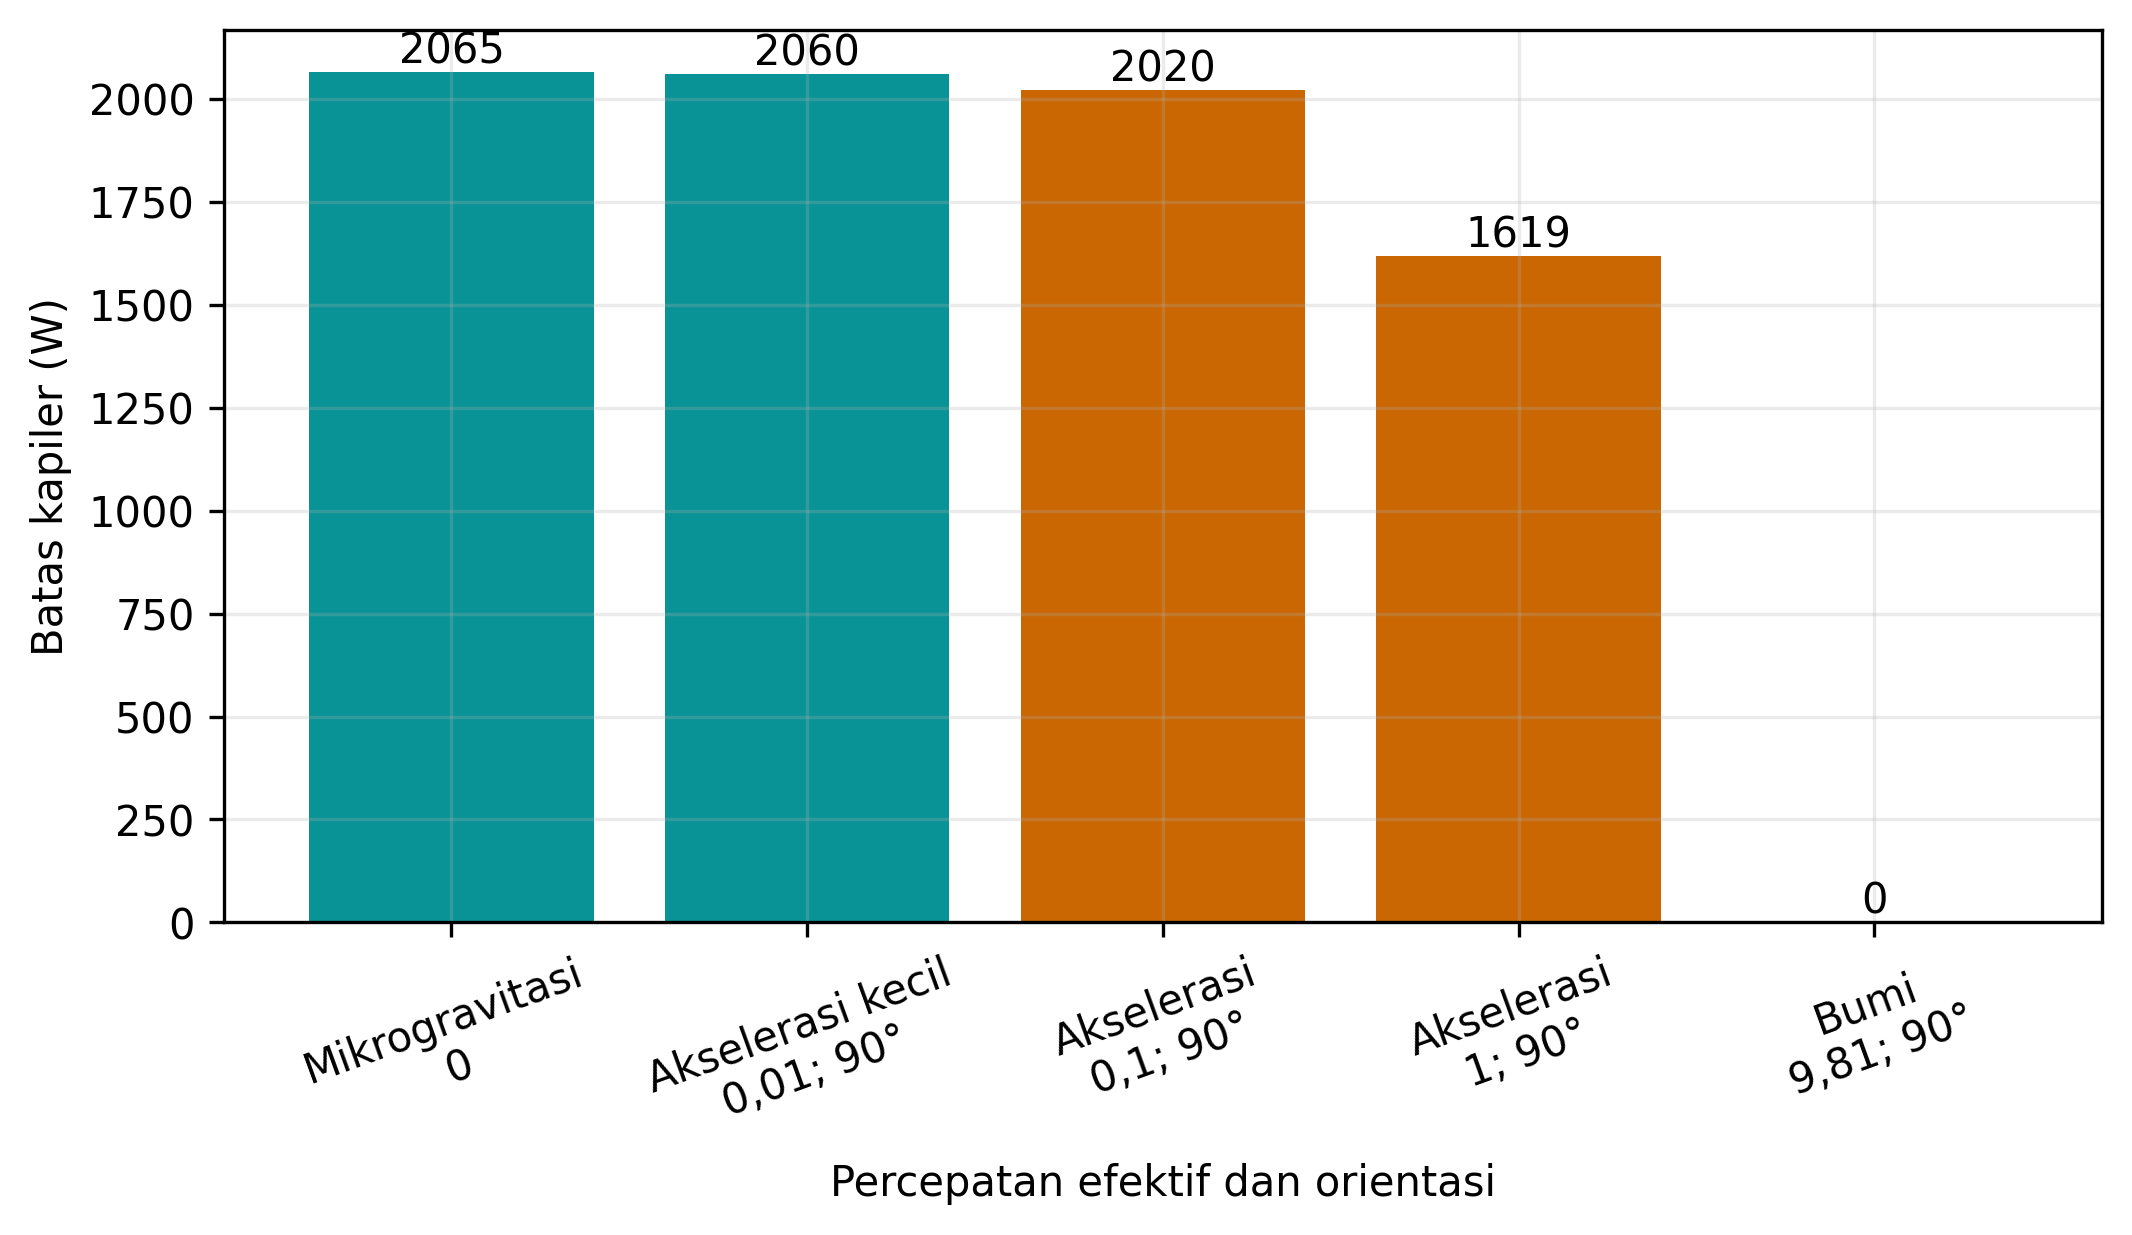
\includegraphics[width=0.92\textwidth,height=\textheight]{figures/pengaruh-gravitasi.png}
\caption{Perbandingan batas kapiler pada mikrogravitasi, beberapa
akselerasi, dan kondisi Bumi dengan orientasi
merugikan.}\label{fig-gravitasi}
}
\end{figure}

Hasil kasus Bumi tidak berarti pipa kalor natrium secara umum tidak
dapat bekerja pada orientasi vertikal. Kesimpulan hanya berlaku untuk
geometri, sumbu, dan orientasi acuan. Pipa dengan pori lebih kecil,
permeabilitas lebih tinggi, panjang lebih pendek, atau orientasi
menguntungkan dapat memiliki perilaku berbeda. Di sisi lain, hasil
mikrogravitasi memperlihatkan alasan kapilaritas penting: sirkulasi
tetap dimungkinkan tanpa kontribusi gravitasi selama neraca Persamaan
(3.17) terpenuhi.

\hypertarget{pengaruh-jari-jari-pori}{%
\section{Pengaruh Jari-Jari Pori}\label{pengaruh-jari-jari-pori}}

Tabel V.6 menunjukkan bahwa pembesaran pori dari 25 µm menjadi 150 µm
menurunkan batas kapiler dari 5544,26 W menjadi 1032,44 W ketika
permeabilitas dibuat tetap. Batas entrainment juga menurun, tetapi
dengan laju berbeda. Pada pori 25 µm, batas entrainment sedikit lebih
tinggi daripada batas kapiler sehingga kapiler masih sedikit lebih
kecil; perbedaan keduanya sangat dekat dan tidak boleh ditafsirkan
melebihi ketidakpastian korelasi.

\begin{longtable}[]{@{}rrr@{}}
\caption{Pengaruh jari-jari pori dengan permeabilitas dipertahankan
tetap.}\tabularnewline
\toprule
Jari-jari pori (µm) & Batas kapiler (W) & Batas entrainment (W) \\
\midrule
\endfirsthead
\toprule
Jari-jari pori (µm) & Batas kapiler (W) & Batas entrainment (W) \\
\midrule
\endhead
25 & 5544,26 & 5563,52 \\
50 & 2974,82 & 3934,00 \\
75 & 2064,88 & 3212,10 \\
100 & 1548,66 & 2781,76 \\
150 & 1032,44 & 2271,30 \\
\bottomrule
\end{longtable}

Hasil ini tidak dapat digunakan untuk menyimpulkan bahwa pori sekecil
mungkin selalu optimal. Pada material nyata, pengecilan pori dapat
menurunkan permeabilitas dan meningkatkan rugi tekanan cairan. Model
sengaja mempertahankan \(K\) untuk isolasi parameter; studi desain
selanjutnya harus menggunakan korelasi eksperimen yang menghubungkan
\(K\), \(r_c\), porositas, dan struktur sumbu.

\hypertarget{konvergensi-grid-dan-verifikasi}{%
\section{Konvergensi Grid dan
Verifikasi}\label{konvergensi-grid-dan-verifikasi}}

Seluruh sepuluh pengujian otomatis berhasil. Pengujian tekanan jenuh
pada 1156 K berada dalam 3\% dari 1 atm, sifat pada 1000 K sesuai
toleransi terhadap nilai acuan, dan margin kapiler pada daya batas
mendekati nol. Program juga menolak permeabilitas nonpositif. Hasil
konvergensi diberikan pada Tabel V.7.

\begin{longtable}[]{@{}
  >{\raggedleft\arraybackslash}p{(\columnwidth - 4\tabcolsep) * \real{0.1558}}
  >{\raggedleft\arraybackslash}p{(\columnwidth - 4\tabcolsep) * \real{0.3247}}
  >{\raggedleft\arraybackslash}p{(\columnwidth - 4\tabcolsep) * \real{0.5195}}@{}}
\caption{Konvergensi jumlah rugi tekanan uap dan cairan pada kasus
acuan.}\tabularnewline
\toprule
\begin{minipage}[b]{\linewidth}\raggedleft
Jumlah sel
\end{minipage} & \begin{minipage}[b]{\linewidth}\raggedleft
Rugi tekanan total (Pa)
\end{minipage} & \begin{minipage}[b]{\linewidth}\raggedleft
Selisih relatif terhadap 1600 sel (\%)
\end{minipage} \\
\midrule
\endfirsthead
\toprule
\begin{minipage}[b]{\linewidth}\raggedleft
Jumlah sel
\end{minipage} & \begin{minipage}[b]{\linewidth}\raggedleft
Rugi tekanan total (Pa)
\end{minipage} & \begin{minipage}[b]{\linewidth}\raggedleft
Selisih relatif terhadap 1600 sel (\%)
\end{minipage} \\
\midrule
\endhead
50 & 1398,9667 & 0,03478 \\
100 & 1399,4535 & \(<10^{-10}\) \\
200 & 1399,4535 & \(<10^{-10}\) \\
400 & 1399,4535 & \(<10^{-10}\) \\
800 & 1399,4535 & \(<10^{-10}\) \\
1600 & 1399,4535 & 0 \\
\bottomrule
\end{longtable}

Perbedaan terbesar hanya 0,03478\% pada 50 sel dan hampir menghilang
setelah 100 sel. Hasil ini masuk akal karena integrand berasal dari
profil linear per bagian dan grid 100 sel atau lebih menempatkan batas
geometri tepat pada titik integrasi. Konvergensi tersebut menunjukkan
konsistensi diskretisasi, bukan bukti bahwa model telah sesuai dengan
fisika eksperimen.

\hypertarget{pembahasan-keterbatasan-model}{%
\section{Pembahasan Keterbatasan
Model}\label{pembahasan-keterbatasan-model}}

Model memberikan hasil yang konsisten dengan dua hipotesis: rugi tekanan
cairan dominan pada kasus acuan dan percepatan merugikan menurunkan
kapasitas kapiler. Namun, beberapa keterbatasan menentukan interpretasi
hasil. Pertama, temperatur uap seragam menghilangkan gradien temperatur
aksial dan resistansi evaporator. Kedua, gas ideal dan viskositas uap
bola keras merupakan penyederhanaan. Ketiga, persamaan faktor gesek
tidak menyelesaikan aliran kompresibel, pusaran, atau interaksi gesek
antarmuka.

Keempat, kondisi jenuh sumbu mengabaikan inventor cairan dan kemungkinan
pengeringan lokal sebelum batas global. Kelima, model pendidihan sangat
sensitif terhadap jari-jari nukleasi dan konduktivitas efektif yang
tidak dikalibrasi. Keenam, start-up beku dan gas takterkondensasi tidak
dicakup meskipun keduanya penting untuk pipa kalor alkali. Ketujuh,
kasus tidak dikopelkan dengan teras reaktor, radiator, atau umpan balik
reaktivitas.

Dengan demikian, istilah yang tepat untuk tahap ini adalah
\textbf{verifikasi kode dan studi numerik}, bukan validasi desain.
Validasi memerlukan data temperatur, daya, tekanan, geometri sumbu, dan
kondisi orientasi dari eksperimen yang terdokumentasi. Ketidakpastian
parameter juga perlu dianalisis sebelum hasil digunakan untuk menetapkan
margin keselamatan.

\hypertarget{kesimpulan-dan-saran}{%
\chapter{KESIMPULAN DAN SARAN}\label{kesimpulan-dan-saran}}

\hypertarget{kesimpulan}{%
\section{Kesimpulan}\label{kesimpulan}}

Berdasarkan pengembangan model dan hasil perhitungan, diperoleh
kesimpulan sebagai berikut.

\begin{enumerate}
\def\labelenumi{\arabic{enumi}.}
\tightlist
\item
  Simulator aliran dua fase tunak satu dimensi telah berhasil disusun
  dalam Python dengan menggabungkan neraca energi, profil laju massa,
  aliran uap, aliran balik cairan Darcy, dan tekanan kapiler. Struktur
  kelas data, keluaran CSV/JSON, gambar otomatis, serta dokumen Quarto
  memungkinkan perhitungan direproduksi.
\item
  Pada kasus acuan 800 W dan 1000 K dalam mikrogravitasi, rugi tekanan
  uap dan cairan masing-masing adalah 103,02 Pa dan 1296,43 Pa. Tekanan
  kapiler 3612,13 Pa memberikan margin 2212,68 Pa. Kecepatan uap
  maksimum adalah 31,87 m/s dan Mach maksimum 0,04105.
\item
  Batas kapiler sebesar 2064,88 W menjadi batas pengatur kasus acuan.
  Batas sonik, entrainment, dan pendidihan masing-masing adalah 7155,53
  W, 3212,10 W, dan 24.232,80 W. Utilisasi daya terhadap batas pengatur
  adalah 38,74\%.
\item
  Peta temperatur menunjukkan batas sonik mengatur pada 800 K,
  entrainment sedikit mengatur pada 900 K, dan kapiler mengatur pada
  1000--1200 K. Kapasitas kapiler mencapai sekitar 2066 W di dekat 1100
  K kemudian menurun menjadi 1969,78 W pada 1200 K.
\item
  Pada orientasi merugikan dan temperatur 1000 K, percepatan 1 m/s²
  menurunkan batas kapiler menjadi 1618,53 W. Kondisi Bumi 9,81 m/s²
  menghasilkan tekanan hidrostatik yang melampaui kapiler untuk geometri
  acuan, sedangkan mikrogravitasi ideal menghilangkan rugi tekanan
  tersebut.
\item
  Sepuluh pengujian otomatis berhasil dan perbedaan rugi tekanan antara
  grid 50 dan 1600 sel hanya 0,03478\%. Hasil ini memverifikasi
  konsistensi implementasi, tetapi belum merupakan validasi
  eksperimental.
\end{enumerate}

\hypertarget{saran}{%
\section{Saran}\label{saran}}

Pengembangan selanjutnya perlu diarahkan pada validasi terhadap data
eksperimen pipa kalor natrium dengan geometri dan kondisi batas yang
terdokumentasi. Model sifat uap sebaiknya ditingkatkan dengan korelasi
yang sesuai untuk campuran monomer dan dimer, sedangkan aliran
kompresibel perlu digunakan pada kasus bermach tinggi. Hubungan
eksperimen antara pori, permeabilitas, porositas, dan konduktivitas
efektif juga diperlukan agar studi desain lebih realistis.

Model dapat dikembangkan menjadi jaringan termal transien yang mencakup
kapasitas panas dinding, start-up beku, gas takterkondensasi, dan
radiator. Untuk analisis reaktor, kopling dengan model teras dan umpan
balik reaktivitas harus dilakukan setelah model pipa tervalidasi.
Analisis ketidakpastian dan sensitivitas global disarankan sebelum hasil
digunakan untuk menetapkan margin desain. Terakhir, studi kegagalan satu
pipa dan propagasinya pada tingkat sistem merupakan kelanjutan penting
yang tidak dapat dijawab oleh model satu pipa ini.

\hypertarget{daftar-pustaka}{%
\chapter*{DAFTAR PUSTAKA}\label{daftar-pustaka}}
\addcontentsline{toc}{chapter}{DAFTAR PUSTAKA}

{[}1{]} G. M. Grover, T. P. Cotter, dan G. F. Erickson. ``Structures of
Very High Thermal Conductance.'' \emph{Journal of Applied Physics},
vol.~35, no. 6, pp.~1990--1991, 1964. DOI: 10.1063/1.1713792.

{[}2{]} T. P. Cotter. \emph{Theory of Heat Pipes}. LA-3246-MS, Los
Alamos Scientific Laboratory, 1965.

{[}3{]} S. W. Chi. \emph{Heat Pipe Theory and Practice: A Sourcebook}.
Washington, DC: Hemisphere Publishing Corporation, 1976.

{[}4{]} A. Faghri. \emph{Heat Pipe Science and Technology}. Washington,
DC: Taylor \& Francis, 1995.

{[}5{]} G. P. Peterson. \emph{An Introduction to Heat Pipes: Modeling,
Testing, and Applications}. New York: John Wiley \& Sons, 1994.

{[}6{]} D. Reay, R. McGlen, dan P. Kew. \emph{Heat Pipes: Theory, Design
and Applications}, ed.~ke-6. Oxford: Butterworth-Heinemann, 2014.

{[}7{]} J. K. Fink dan L. Leibowitz. \emph{Thermodynamic and Transport
Properties of Sodium Liquid and Vapor}. ANL/RE-95/2, Argonne National
Laboratory, 1995.

{[}8{]} B. H. Yan, C. Wang, dan L. Li. ``The Technology of Micro Heat
Pipe Cooled Reactor: A Review.'' \emph{Annals of Nuclear Energy},
vol.~135, 106948, 2020. DOI: 10.1016/j.anucene.2019.106948.

{[}9{]} E. Wang, T. Ren, dan L. Li. ``Review of Reactor Conceptual
Design and Thermal Hydraulic Characteristics for Heat Pipe in Nuclear
Systems.'' \emph{Frontiers in Energy Research}, vol.~11, 1264168, 2023.
DOI: 10.3389/fenrg.2023.1264168.

{[}10{]} C. Wang, H. Sun, S. Tang, W. Tian, S. Qiu, dan G. Su.
``Thermal-Hydraulic Analysis of a New Conceptual Heat Pipe Cooled Small
Nuclear Reactor System.'' \emph{Nuclear Engineering and Technology},
vol.~52, no. 1, pp.~19--26, 2020. DOI: 10.1016/j.net.2019.06.021.

{[}11{]} K. A. Woloshun, M. A. Merrigan, dan E. D. Best. \emph{HTPIPE: A
Steady-State Heat Pipe Analysis Program---A User's Manual}. Los Alamos
National Laboratory, 1988.

{[}12{]} Z. Zhang, C. Wang, K. Guo, J. Huang, S. Qiu, dan G. Su.
``HEART, a Specific Code for Thermal-Electrical Analysis of Heat Pipe
Cooled Nuclear Reactor.'' \emph{International Journal of Thermal
Sciences}, vol.~179, 107666, 2022. DOI:
10.1016/j.ijthermalsci.2022.107666.

{[}13{]} S. Wahlquist dan kolaborator. ``A Critical Review of Heat Pipe
Experiments in Nuclear Energy Applications.'' \emph{Nuclear Science and
Engineering}, vol.~197, no. 5, pp.~719--752, 2023.

{[}14{]} C. R. Harris et al.~``Array Programming with NumPy.''
\emph{Nature}, vol.~585, pp.~357--362, 2020. DOI:
10.1038/s41586-020-2649-2.

{[}15{]} J. D. Hunter. ``Matplotlib: A 2D Graphics Environment.''
\emph{Computing in Science \& Engineering}, vol.~9, no. 3, pp.~90--95,
2007. DOI: 10.1109/MCSE.2007.55.

\appendix

\hypertarget{listing-program-simulator}{%
\chapter{LISTING PROGRAM SIMULATOR}\label{listing-program-simulator}}

Lampiran ini memuat sumber lengkap \texttt{src/heatpipe\_simulator.py}.
Program menggunakan satuan SI dan menghasilkan ulang seluruh data serta
gambar yang dibahas pada Bab V.

\begin{Shaded}
\begin{Highlighting}[]
\CommentTok{\#!/usr/bin/env python3}
\CommentTok{"""Reduced{-}order, steady 1{-}D sodium heat{-}pipe simulator.}

\CommentTok{The model couples axial vapor flow, Darcy liquid return through a homogeneous}
\CommentTok{wick, and capillary pressure. It is intended for transparent thesis case}
\CommentTok{studies, not design certification or transient/CFD analysis.}

\CommentTok{Sodium correlations follow Fink and Leibowitz (1995), ANL/RE{-}95/2.}
\CommentTok{All internal calculations use SI units.}
\CommentTok{"""}
\ImportTok{from}\NormalTok{ \_\_future\_\_ }\ImportTok{import}\NormalTok{ annotations}

\ImportTok{import}\NormalTok{ argparse}
\ImportTok{import}\NormalTok{ csv}
\ImportTok{import}\NormalTok{ json}
\ImportTok{import}\NormalTok{ math}
\ImportTok{import}\NormalTok{ warnings}
\ImportTok{from}\NormalTok{ dataclasses }\ImportTok{import}\NormalTok{ asdict, dataclass, replace}
\ImportTok{from}\NormalTok{ pathlib }\ImportTok{import}\NormalTok{ Path}
\ImportTok{from}\NormalTok{ typing }\ImportTok{import}\NormalTok{ Iterable}

\ImportTok{import}\NormalTok{ matplotlib}
\NormalTok{matplotlib.use(}\StringTok{"Agg"}\NormalTok{)}
\ImportTok{import}\NormalTok{ matplotlib.pyplot }\ImportTok{as}\NormalTok{ plt}
\ImportTok{import}\NormalTok{ numpy }\ImportTok{as}\NormalTok{ np}

\NormalTok{R\_UNIVERSAL }\OperatorTok{=} \FloatTok{8.314462618}  \CommentTok{\# J mol{-}1 K{-}1}
\NormalTok{MOLAR\_MASS\_NA }\OperatorTok{=} \FloatTok{22.98976928e{-}3}  \CommentTok{\# kg mol{-}1}
\NormalTok{K\_BOLTZMANN }\OperatorTok{=} \FloatTok{1.380649e{-}23}  \CommentTok{\# J K{-}1}


\AttributeTok{@dataclass}\NormalTok{(frozen}\OperatorTok{=}\VariableTok{True}\NormalTok{)}
\KeywordTok{class}\NormalTok{ SodiumProperties:}
    \CommentTok{"""Saturated{-}sodium properties; recommended thesis range: 800{-}{-}1400 K."""}

\NormalTok{    temperature: }\BuiltInTok{float}

    \KeywordTok{def}\NormalTok{ \_\_post\_init\_\_(}\VariableTok{self}\NormalTok{) }\OperatorTok{{-}\textgreater{}} \VariableTok{None}\NormalTok{:}
        \ControlFlowTok{if} \KeywordTok{not} \FloatTok{371.0} \OperatorTok{\textless{}=} \VariableTok{self}\NormalTok{.temperature }\OperatorTok{\textless{}} \FloatTok{2503.7}\NormalTok{:}
            \ControlFlowTok{raise} \PreprocessorTok{ValueError}\NormalTok{(}\StringTok{"Temperature must be in [371, 2503.7) K."}\NormalTok{)}
        \ControlFlowTok{if} \KeywordTok{not} \FloatTok{800.0} \OperatorTok{\textless{}=} \VariableTok{self}\NormalTok{.temperature }\OperatorTok{\textless{}=} \FloatTok{1400.0}\NormalTok{:}
\NormalTok{            warnings.warn(}
                \SpecialStringTok{f"T=}\SpecialCharTok{\{}\VariableTok{self}\SpecialCharTok{.}\NormalTok{temperature}\SpecialCharTok{:.1f\}}\SpecialStringTok{ K is outside the thesis validation "}
                \StringTok{"target of 800{-}{-}1400 K; check extrapolation."}\NormalTok{,}
\NormalTok{                stacklevel}\OperatorTok{=}\DecValTok{2}\NormalTok{,}
\NormalTok{            )}

    \AttributeTok{@property}
    \KeywordTok{def}\NormalTok{ pressure(}\VariableTok{self}\NormalTok{) }\OperatorTok{{-}\textgreater{}} \BuiltInTok{float}\NormalTok{:}
        \CommentTok{"""Saturation pressure (Pa), Browning{-}{-}Potter correlation."""}
\NormalTok{        ln\_p\_mpa }\OperatorTok{=}\NormalTok{ (}
            \FloatTok{11.9463} \OperatorTok{{-}} \FloatTok{12633.73} \OperatorTok{/} \VariableTok{self}\NormalTok{.temperature}
            \OperatorTok{{-}} \FloatTok{0.4672} \OperatorTok{*}\NormalTok{ math.log(}\VariableTok{self}\NormalTok{.temperature)}
\NormalTok{        )}
        \ControlFlowTok{return}\NormalTok{ math.exp(ln\_p\_mpa) }\OperatorTok{*} \FloatTok{1.0e6}

    \AttributeTok{@property}
    \KeywordTok{def}\NormalTok{ latent\_heat(}\VariableTok{self}\NormalTok{) }\OperatorTok{{-}\textgreater{}} \BuiltInTok{float}\NormalTok{:}
        \CommentTok{"""Specific enthalpy of vaporization (J kg{-}1)."""}
\NormalTok{        tau }\OperatorTok{=} \FloatTok{1.0} \OperatorTok{{-}} \VariableTok{self}\NormalTok{.temperature }\OperatorTok{/} \FloatTok{2503.7}
\NormalTok{        h\_fg\_kj\_kg }\OperatorTok{=} \FloatTok{393.37} \OperatorTok{*}\NormalTok{ tau }\OperatorTok{+} \FloatTok{4398.6} \OperatorTok{*}\NormalTok{ tau}\OperatorTok{**}\FloatTok{0.29302}
        \ControlFlowTok{return}\NormalTok{ h\_fg\_kj\_kg }\OperatorTok{*} \FloatTok{1000.0}

    \AttributeTok{@property}
    \KeywordTok{def}\NormalTok{ liquid\_density(}\VariableTok{self}\NormalTok{) }\OperatorTok{{-}\textgreater{}} \BuiltInTok{float}\NormalTok{:}
        \CommentTok{"""Saturated liquid density (kg m{-}3)."""}
\NormalTok{        tau }\OperatorTok{=} \FloatTok{1.0} \OperatorTok{{-}} \VariableTok{self}\NormalTok{.temperature }\OperatorTok{/} \FloatTok{2503.7}
        \ControlFlowTok{return} \FloatTok{219.0} \OperatorTok{+} \FloatTok{275.32} \OperatorTok{*}\NormalTok{ tau }\OperatorTok{+} \FloatTok{511.58} \OperatorTok{*}\NormalTok{ math.sqrt(tau)}

    \AttributeTok{@property}
    \KeywordTok{def}\NormalTok{ vapor\_density(}\VariableTok{self}\NormalTok{) }\OperatorTok{{-}\textgreater{}} \BuiltInTok{float}\NormalTok{:}
        \CommentTok{"""Ideal{-}gas approximation to saturated vapor density (kg m{-}3)."""}
        \ControlFlowTok{return}\NormalTok{ (}
            \VariableTok{self}\NormalTok{.pressure }\OperatorTok{*}\NormalTok{ MOLAR\_MASS\_NA}
            \OperatorTok{/}\NormalTok{ (R\_UNIVERSAL }\OperatorTok{*} \VariableTok{self}\NormalTok{.temperature)}
\NormalTok{        )}

    \AttributeTok{@property}
    \KeywordTok{def}\NormalTok{ liquid\_viscosity(}\VariableTok{self}\NormalTok{) }\OperatorTok{{-}\textgreater{}} \BuiltInTok{float}\NormalTok{:}
        \CommentTok{"""Dynamic viscosity of liquid sodium (Pa s)."""}
        \ControlFlowTok{return}\NormalTok{ math.exp(}
            \OperatorTok{{-}}\FloatTok{6.4406} \OperatorTok{{-}} \FloatTok{0.3958} \OperatorTok{*}\NormalTok{ math.log(}\VariableTok{self}\NormalTok{.temperature)}
            \OperatorTok{+} \FloatTok{556.835} \OperatorTok{/} \VariableTok{self}\NormalTok{.temperature}
\NormalTok{        )}

    \AttributeTok{@property}
    \KeywordTok{def}\NormalTok{ vapor\_viscosity(}\VariableTok{self}\NormalTok{) }\OperatorTok{{-}\textgreater{}} \BuiltInTok{float}\NormalTok{:}
        \CommentTok{"""Hard{-}sphere dilute{-}gas estimate of vapor viscosity (Pa s).}

\CommentTok{        A 4.0 Angstrom collision diameter is used because the recommended}
\CommentTok{        liquid{-}property report does not provide a sodium{-}vapor viscosity}
\CommentTok{        correlation. Replace this approximation for high{-}fidelity studies.}
\CommentTok{        """}
\NormalTok{        mass }\OperatorTok{=}\NormalTok{ MOLAR\_MASS\_NA }\OperatorTok{/} \FloatTok{6.02214076e23}
\NormalTok{        diameter }\OperatorTok{=} \FloatTok{4.0e{-}10}
        \ControlFlowTok{return}\NormalTok{ (}
            \FloatTok{5.0} \OperatorTok{/}\NormalTok{ (}\FloatTok{16.0} \OperatorTok{*}\NormalTok{ diameter}\OperatorTok{**}\DecValTok{2}\NormalTok{)}
            \OperatorTok{*}\NormalTok{ math.sqrt(mass }\OperatorTok{*}\NormalTok{ K\_BOLTZMANN }\OperatorTok{*} \VariableTok{self}\NormalTok{.temperature }\OperatorTok{/}\NormalTok{ math.pi)}
\NormalTok{        )}

    \AttributeTok{@property}
    \KeywordTok{def}\NormalTok{ surface\_tension(}\VariableTok{self}\NormalTok{) }\OperatorTok{{-}\textgreater{}} \BuiltInTok{float}\NormalTok{:}
        \CommentTok{"""Liquid surface tension (N m{-}1), Van der Waals correlation."""}
        \ControlFlowTok{return}\NormalTok{ (}
            \FloatTok{240.5e{-}3} \OperatorTok{*}\NormalTok{ (}\FloatTok{1.0} \OperatorTok{{-}} \VariableTok{self}\NormalTok{.temperature }\OperatorTok{/} \FloatTok{2503.7}\NormalTok{)}\OperatorTok{**}\FloatTok{1.126}
\NormalTok{        )}

    \AttributeTok{@property}
    \KeywordTok{def}\NormalTok{ liquid\_conductivity(}\VariableTok{self}\NormalTok{) }\OperatorTok{{-}\textgreater{}} \BuiltInTok{float}\NormalTok{:}
        \CommentTok{"""Liquid thermal conductivity (W m{-}1 K{-}1)."""}
\NormalTok{        t }\OperatorTok{=} \VariableTok{self}\NormalTok{.temperature}
        \ControlFlowTok{return}\NormalTok{ (}
            \FloatTok{124.67} \OperatorTok{{-}} \FloatTok{0.11381} \OperatorTok{*}\NormalTok{ t }\OperatorTok{+} \FloatTok{5.5226e{-}5} \OperatorTok{*}\NormalTok{ t}\OperatorTok{**}\DecValTok{2}
            \OperatorTok{{-}} \FloatTok{1.1842e{-}8} \OperatorTok{*}\NormalTok{ t}\OperatorTok{**}\DecValTok{3}
\NormalTok{        )}

    \AttributeTok{@property}
    \KeywordTok{def}\NormalTok{ specific\_gas\_constant(}\VariableTok{self}\NormalTok{) }\OperatorTok{{-}\textgreater{}} \BuiltInTok{float}\NormalTok{:}
        \ControlFlowTok{return}\NormalTok{ R\_UNIVERSAL }\OperatorTok{/}\NormalTok{ MOLAR\_MASS\_NA}

    \AttributeTok{@property}
    \KeywordTok{def}\NormalTok{ sound\_speed(}\VariableTok{self}\NormalTok{) }\OperatorTok{{-}\textgreater{}} \BuiltInTok{float}\NormalTok{:}
        \CommentTok{"""Monatomic ideal{-}gas sound{-}speed estimate (m s{-}1)."""}
        \ControlFlowTok{return}\NormalTok{ math.sqrt((}\FloatTok{5.0} \OperatorTok{/} \FloatTok{3.0}\NormalTok{) }\OperatorTok{*} \VariableTok{self}\NormalTok{.specific\_gas\_constant }\OperatorTok{*} \VariableTok{self}\NormalTok{.temperature)}

    \KeywordTok{def}\NormalTok{ summary(}\VariableTok{self}\NormalTok{) }\OperatorTok{{-}\textgreater{}} \BuiltInTok{dict}\NormalTok{[}\BuiltInTok{str}\NormalTok{, }\BuiltInTok{float}\NormalTok{]:}
        \ControlFlowTok{return}\NormalTok{ \{}
            \StringTok{"temperature\_K"}\NormalTok{: }\VariableTok{self}\NormalTok{.temperature,}
            \StringTok{"saturation\_pressure\_Pa"}\NormalTok{: }\VariableTok{self}\NormalTok{.pressure,}
            \StringTok{"latent\_heat\_J\_kg"}\NormalTok{: }\VariableTok{self}\NormalTok{.latent\_heat,}
            \StringTok{"liquid\_density\_kg\_m3"}\NormalTok{: }\VariableTok{self}\NormalTok{.liquid\_density,}
            \StringTok{"vapor\_density\_kg\_m3"}\NormalTok{: }\VariableTok{self}\NormalTok{.vapor\_density,}
            \StringTok{"liquid\_viscosity\_Pa\_s"}\NormalTok{: }\VariableTok{self}\NormalTok{.liquid\_viscosity,}
            \StringTok{"vapor\_viscosity\_Pa\_s"}\NormalTok{: }\VariableTok{self}\NormalTok{.vapor\_viscosity,}
            \StringTok{"surface\_tension\_N\_m"}\NormalTok{: }\VariableTok{self}\NormalTok{.surface\_tension,}
            \StringTok{"liquid\_conductivity\_W\_mK"}\NormalTok{: }\VariableTok{self}\NormalTok{.liquid\_conductivity,}
            \StringTok{"sound\_speed\_m\_s"}\NormalTok{: }\VariableTok{self}\NormalTok{.sound\_speed,}
\NormalTok{        \}}


\AttributeTok{@dataclass}\NormalTok{(frozen}\OperatorTok{=}\VariableTok{True}\NormalTok{)}
\KeywordTok{class}\NormalTok{ HeatPipeGeometry:}
\NormalTok{    evaporator\_length: }\BuiltInTok{float} \OperatorTok{=} \FloatTok{0.25}
\NormalTok{    adiabatic\_length: }\BuiltInTok{float} \OperatorTok{=} \FloatTok{0.15}
\NormalTok{    condenser\_length: }\BuiltInTok{float} \OperatorTok{=} \FloatTok{0.60}
\NormalTok{    vapor\_diameter: }\BuiltInTok{float} \OperatorTok{=} \FloatTok{0.012}
\NormalTok{    wick\_thickness: }\BuiltInTok{float} \OperatorTok{=} \FloatTok{0.001}
\NormalTok{    pore\_radius: }\BuiltInTok{float} \OperatorTok{=} \FloatTok{75.0e{-}6}
\NormalTok{    permeability: }\BuiltInTok{float} \OperatorTok{=} \FloatTok{5.0e{-}10}
\NormalTok{    contact\_angle\_deg: }\BuiltInTok{float} \OperatorTok{=} \FloatTok{0.0}
\NormalTok{    effective\_wick\_conductivity: }\BuiltInTok{float} \OperatorTok{=} \FloatTok{10.0}
\NormalTok{    bubble\_radius: }\BuiltInTok{float} \OperatorTok{=} \FloatTok{5.0e{-}6}

    \KeywordTok{def}\NormalTok{ \_\_post\_init\_\_(}\VariableTok{self}\NormalTok{) }\OperatorTok{{-}\textgreater{}} \VariableTok{None}\NormalTok{:}
\NormalTok{        positive }\OperatorTok{=}\NormalTok{ \{}
\NormalTok{            key: value }\ControlFlowTok{for}\NormalTok{ key, value }\KeywordTok{in}\NormalTok{ asdict(}\VariableTok{self}\NormalTok{).items()}
            \ControlFlowTok{if}\NormalTok{ key }\OperatorTok{!=} \StringTok{"contact\_angle\_deg"}
\NormalTok{        \}}
        \ControlFlowTok{if} \BuiltInTok{any}\NormalTok{(value }\OperatorTok{\textless{}=} \FloatTok{0.0} \ControlFlowTok{for}\NormalTok{ value }\KeywordTok{in}\NormalTok{ positive.values()):}
            \ControlFlowTok{raise} \PreprocessorTok{ValueError}\NormalTok{(}\StringTok{"All geometry and wick properties must be positive."}\NormalTok{)}
        \ControlFlowTok{if} \KeywordTok{not} \FloatTok{0.0} \OperatorTok{\textless{}=} \VariableTok{self}\NormalTok{.contact\_angle\_deg }\OperatorTok{\textless{}} \FloatTok{90.0}\NormalTok{:}
            \ControlFlowTok{raise} \PreprocessorTok{ValueError}\NormalTok{(}\StringTok{"Contact angle must be in [0, 90) degrees."}\NormalTok{)}

    \AttributeTok{@property}
    \KeywordTok{def}\NormalTok{ total\_length(}\VariableTok{self}\NormalTok{) }\OperatorTok{{-}\textgreater{}} \BuiltInTok{float}\NormalTok{:}
        \ControlFlowTok{return} \VariableTok{self}\NormalTok{.evaporator\_length }\OperatorTok{+} \VariableTok{self}\NormalTok{.adiabatic\_length }\OperatorTok{+} \VariableTok{self}\NormalTok{.condenser\_length}

    \AttributeTok{@property}
    \KeywordTok{def}\NormalTok{ effective\_length(}\VariableTok{self}\NormalTok{) }\OperatorTok{{-}\textgreater{}} \BuiltInTok{float}\NormalTok{:}
        \ControlFlowTok{return}\NormalTok{ (}
            \VariableTok{self}\NormalTok{.evaporator\_length }\OperatorTok{/} \FloatTok{2.0} \OperatorTok{+} \VariableTok{self}\NormalTok{.adiabatic\_length}
            \OperatorTok{+} \VariableTok{self}\NormalTok{.condenser\_length }\OperatorTok{/} \FloatTok{2.0}
\NormalTok{        )}

    \AttributeTok{@property}
    \KeywordTok{def}\NormalTok{ vapor\_area(}\VariableTok{self}\NormalTok{) }\OperatorTok{{-}\textgreater{}} \BuiltInTok{float}\NormalTok{:}
        \ControlFlowTok{return}\NormalTok{ math.pi }\OperatorTok{*} \VariableTok{self}\NormalTok{.vapor\_diameter}\OperatorTok{**}\DecValTok{2} \OperatorTok{/} \FloatTok{4.0}

    \AttributeTok{@property}
    \KeywordTok{def}\NormalTok{ wick\_area(}\VariableTok{self}\NormalTok{) }\OperatorTok{{-}\textgreater{}} \BuiltInTok{float}\NormalTok{:}
\NormalTok{        r\_v }\OperatorTok{=} \VariableTok{self}\NormalTok{.vapor\_diameter }\OperatorTok{/} \FloatTok{2.0}
        \ControlFlowTok{return}\NormalTok{ math.pi }\OperatorTok{*}\NormalTok{ ((r\_v }\OperatorTok{+} \VariableTok{self}\NormalTok{.wick\_thickness)}\OperatorTok{**}\DecValTok{2} \OperatorTok{{-}}\NormalTok{ r\_v}\OperatorTok{**}\DecValTok{2}\NormalTok{)}

    \AttributeTok{@property}
    \KeywordTok{def}\NormalTok{ capillary\_pressure(}\VariableTok{self}\NormalTok{) }\OperatorTok{{-}\textgreater{}} \BuiltInTok{float}\NormalTok{:}
        \ControlFlowTok{raise} \PreprocessorTok{AttributeError}\NormalTok{(}\StringTok{"Capillary pressure also requires fluid temperature."}\NormalTok{)}


\AttributeTok{@dataclass}\NormalTok{(frozen}\OperatorTok{=}\VariableTok{True}\NormalTok{)}
\KeywordTok{class}\NormalTok{ OperatingConditions:}
\NormalTok{    heat\_input: }\BuiltInTok{float} \OperatorTok{=} \FloatTok{800.0}
\NormalTok{    sink\_temperature: }\BuiltInTok{float} \OperatorTok{=} \FloatTok{700.0}
\NormalTok{    condenser\_resistance: }\BuiltInTok{float} \OperatorTok{=} \FloatTok{0.375}
\NormalTok{    gravity: }\BuiltInTok{float} \OperatorTok{=} \FloatTok{0.0}
\NormalTok{    tilt\_deg: }\BuiltInTok{float} \OperatorTok{=} \FloatTok{0.0}
\NormalTok{    cells: }\BuiltInTok{int} \OperatorTok{=} \DecValTok{400}

    \KeywordTok{def}\NormalTok{ \_\_post\_init\_\_(}\VariableTok{self}\NormalTok{) }\OperatorTok{{-}\textgreater{}} \VariableTok{None}\NormalTok{:}
        \ControlFlowTok{if} \VariableTok{self}\NormalTok{.heat\_input }\OperatorTok{\textless{}} \FloatTok{0.0} \KeywordTok{or} \VariableTok{self}\NormalTok{.sink\_temperature }\OperatorTok{\textless{}=} \FloatTok{0.0}\NormalTok{:}
            \ControlFlowTok{raise} \PreprocessorTok{ValueError}\NormalTok{(}
                \StringTok{"Heat input must be nonnegative and sink temperature positive."}
\NormalTok{            )}
        \ControlFlowTok{if} \VariableTok{self}\NormalTok{.condenser\_resistance }\OperatorTok{\textless{}=} \FloatTok{0.0} \KeywordTok{or} \VariableTok{self}\NormalTok{.gravity }\OperatorTok{\textless{}} \FloatTok{0.0}\NormalTok{:}
            \ControlFlowTok{raise} \PreprocessorTok{ValueError}\NormalTok{(}
                \StringTok{"Condenser resistance must be positive and gravity nonnegative."}
\NormalTok{            )}
        \ControlFlowTok{if} \VariableTok{self}\NormalTok{.cells }\OperatorTok{\textless{}} \DecValTok{20}\NormalTok{:}
            \ControlFlowTok{raise} \PreprocessorTok{ValueError}\NormalTok{(}\StringTok{"Use at least 20 axial cells."}\NormalTok{)}

    \AttributeTok{@property}
    \KeywordTok{def}\NormalTok{ operating\_temperature(}\VariableTok{self}\NormalTok{) }\OperatorTok{{-}\textgreater{}} \BuiltInTok{float}\NormalTok{:}
        \ControlFlowTok{return} \VariableTok{self}\NormalTok{.sink\_temperature }\OperatorTok{+} \VariableTok{self}\NormalTok{.condenser\_resistance }\OperatorTok{*} \VariableTok{self}\NormalTok{.heat\_input}


\AttributeTok{@dataclass}
\KeywordTok{class}\NormalTok{ SimulationResult:}
\NormalTok{    x: np.ndarray}
\NormalTok{    section: np.ndarray}
\NormalTok{    axial\_heat\_flow: np.ndarray}
\NormalTok{    mass\_flow: np.ndarray}
\NormalTok{    vapor\_velocity: np.ndarray}
\NormalTok{    reynolds: np.ndarray}
\NormalTok{    mach: np.ndarray}
\NormalTok{    vapor\_pressure\_drop: np.ndarray}
\NormalTok{    liquid\_pressure\_drop: np.ndarray}
\NormalTok{    summary: }\BuiltInTok{dict}\NormalTok{[}\BuiltInTok{str}\NormalTok{, }\BuiltInTok{float} \OperatorTok{|} \BuiltInTok{str} \OperatorTok{|} \BuiltInTok{bool}\NormalTok{]}


\KeywordTok{def}\NormalTok{ capillary\_pressure(geometry: HeatPipeGeometry, fluid: SodiumProperties) }\OperatorTok{{-}\textgreater{}} \BuiltInTok{float}\NormalTok{:}
    \ControlFlowTok{return}\NormalTok{ (}
        \FloatTok{2.0} \OperatorTok{*}\NormalTok{ fluid.surface\_tension}
        \OperatorTok{*}\NormalTok{ math.cos(math.radians(geometry.contact\_angle\_deg))}
        \OperatorTok{/}\NormalTok{ geometry.pore\_radius}
\NormalTok{    )}


\KeywordTok{def}\NormalTok{ axial\_heat\_profile(}
\NormalTok{    x: np.ndarray, heat\_input: }\BuiltInTok{float}\NormalTok{, geometry: HeatPipeGeometry,}
\NormalTok{) }\OperatorTok{{-}\textgreater{}}\NormalTok{ np.ndarray:}
    \CommentTok{"""Heat carried by vapor; x=0 is the closed evaporator end."""}
\NormalTok{    le, la, lc }\OperatorTok{=}\NormalTok{ (}
\NormalTok{        geometry.evaporator\_length,}
\NormalTok{        geometry.adiabatic\_length,}
\NormalTok{        geometry.condenser\_length,}
\NormalTok{    )}
\NormalTok{    q }\OperatorTok{=}\NormalTok{ np.empty\_like(x)}
\NormalTok{    evap }\OperatorTok{=}\NormalTok{ x }\OperatorTok{\textless{}=}\NormalTok{ le}
\NormalTok{    adiab }\OperatorTok{=}\NormalTok{ (x }\OperatorTok{\textgreater{}}\NormalTok{ le) }\OperatorTok{\&}\NormalTok{ (x }\OperatorTok{\textless{}=}\NormalTok{ le }\OperatorTok{+}\NormalTok{ la)}
\NormalTok{    cond }\OperatorTok{=}\NormalTok{ x }\OperatorTok{\textgreater{}}\NormalTok{ le }\OperatorTok{+}\NormalTok{ la}
\NormalTok{    q[evap] }\OperatorTok{=}\NormalTok{ heat\_input }\OperatorTok{*}\NormalTok{ x[evap] }\OperatorTok{/}\NormalTok{ le}
\NormalTok{    q[adiab] }\OperatorTok{=}\NormalTok{ heat\_input}
\NormalTok{    q[cond] }\OperatorTok{=}\NormalTok{ heat\_input }\OperatorTok{*}\NormalTok{ (}\FloatTok{1.0} \OperatorTok{{-}}\NormalTok{ (x[cond] }\OperatorTok{{-}}\NormalTok{ le }\OperatorTok{{-}}\NormalTok{ la) }\OperatorTok{/}\NormalTok{ lc)}
    \ControlFlowTok{return}\NormalTok{ np.maximum(q, }\FloatTok{0.0}\NormalTok{)}


\KeywordTok{def}\NormalTok{ \_cumulative\_trapezoid(y: np.ndarray, x: np.ndarray) }\OperatorTok{{-}\textgreater{}}\NormalTok{ np.ndarray:}
\NormalTok{    result }\OperatorTok{=}\NormalTok{ np.zeros\_like(y)}
\NormalTok{    result[}\DecValTok{1}\NormalTok{:] }\OperatorTok{=}\NormalTok{ np.cumsum(}\FloatTok{0.5} \OperatorTok{*}\NormalTok{ (y[}\DecValTok{1}\NormalTok{:] }\OperatorTok{+}\NormalTok{ y[:}\OperatorTok{{-}}\DecValTok{1}\NormalTok{]) }\OperatorTok{*}\NormalTok{ np.diff(x))}
    \ControlFlowTok{return}\NormalTok{ result}


\KeywordTok{def}\NormalTok{ simulate\_at\_temperature(}
\NormalTok{    geometry: HeatPipeGeometry,}
\NormalTok{    conditions: OperatingConditions,}
\NormalTok{    temperature: }\BuiltInTok{float}\NormalTok{,}
\NormalTok{) }\OperatorTok{{-}\textgreater{}}\NormalTok{ SimulationResult:}
    \CommentTok{"""Solve the steady axial profile at a prescribed saturation temperature."""}
\NormalTok{    fluid }\OperatorTok{=}\NormalTok{ SodiumProperties(temperature)}
\NormalTok{    x }\OperatorTok{=}\NormalTok{ np.linspace(}\FloatTok{0.0}\NormalTok{, geometry.total\_length, conditions.cells }\OperatorTok{+} \DecValTok{1}\NormalTok{)}
\NormalTok{    q }\OperatorTok{=}\NormalTok{ axial\_heat\_profile(x, conditions.heat\_input, geometry)}
\NormalTok{    mdot }\OperatorTok{=}\NormalTok{ q }\OperatorTok{/}\NormalTok{ fluid.latent\_heat}
\NormalTok{    velocity }\OperatorTok{=}\NormalTok{ mdot }\OperatorTok{/}\NormalTok{ (fluid.vapor\_density }\OperatorTok{*}\NormalTok{ geometry.vapor\_area)}
\NormalTok{    reynolds }\OperatorTok{=}\NormalTok{ (}
\NormalTok{        fluid.vapor\_density }\OperatorTok{*}\NormalTok{ velocity }\OperatorTok{*}\NormalTok{ geometry.vapor\_diameter}
        \OperatorTok{/}\NormalTok{ fluid.vapor\_viscosity}
\NormalTok{    )}
\NormalTok{    mach }\OperatorTok{=}\NormalTok{ velocity }\OperatorTok{/}\NormalTok{ fluid.sound\_speed}
\NormalTok{    friction }\OperatorTok{=}\NormalTok{ np.where(}
\NormalTok{        reynolds }\OperatorTok{\textless{}} \FloatTok{2300.0}\NormalTok{,}
        \FloatTok{64.0} \OperatorTok{/}\NormalTok{ np.maximum(reynolds, }\FloatTok{1.0e{-}12}\NormalTok{),}
        \FloatTok{0.3164} \OperatorTok{/}\NormalTok{ np.maximum(reynolds, }\FloatTok{1.0e{-}12}\NormalTok{)}\OperatorTok{**}\FloatTok{0.25}\NormalTok{,}
\NormalTok{    )}
\NormalTok{    friction }\OperatorTok{=}\NormalTok{ np.where(reynolds }\OperatorTok{\textless{}} \FloatTok{1.0e{-}12}\NormalTok{, }\FloatTok{0.0}\NormalTok{, friction)}
\NormalTok{    dpv\_dx }\OperatorTok{=}\NormalTok{ (}
\NormalTok{        friction }\OperatorTok{/}\NormalTok{ geometry.vapor\_diameter}
        \OperatorTok{*} \FloatTok{0.5} \OperatorTok{*}\NormalTok{ fluid.vapor\_density }\OperatorTok{*}\NormalTok{ velocity}\OperatorTok{**}\DecValTok{2}
\NormalTok{    )}
\NormalTok{    dpl\_dx }\OperatorTok{=}\NormalTok{ (}
\NormalTok{        fluid.liquid\_viscosity }\OperatorTok{*}\NormalTok{ mdot}
        \OperatorTok{/}\NormalTok{ (fluid.liquid\_density }\OperatorTok{*}\NormalTok{ geometry.permeability }\OperatorTok{*}\NormalTok{ geometry.wick\_area)}
\NormalTok{    )}
\NormalTok{    dpv }\OperatorTok{=}\NormalTok{ \_cumulative\_trapezoid(dpv\_dx, x)}
\NormalTok{    dpl }\OperatorTok{=}\NormalTok{ \_cumulative\_trapezoid(dpl\_dx, x)}
\NormalTok{    dp\_gravity }\OperatorTok{=}\NormalTok{ (}
\NormalTok{        fluid.liquid\_density }\OperatorTok{*}\NormalTok{ conditions.gravity }\OperatorTok{*}\NormalTok{ geometry.total\_length}
        \OperatorTok{*}\NormalTok{ math.sin(math.radians(conditions.tilt\_deg))}
\NormalTok{    )}
\NormalTok{    p\_cap }\OperatorTok{=}\NormalTok{ capillary\_pressure(geometry, fluid)}
\NormalTok{    margin }\OperatorTok{=}\NormalTok{ p\_cap }\OperatorTok{{-}}\NormalTok{ dpv[}\OperatorTok{{-}}\DecValTok{1}\NormalTok{] }\OperatorTok{{-}}\NormalTok{ dpl[}\OperatorTok{{-}}\DecValTok{1}\NormalTok{] }\OperatorTok{{-}}\NormalTok{ dp\_gravity}

    \CommentTok{\# Engineering screening limits (Faghri/Chi{-}style reduced{-}order expressions).}
\NormalTok{    q\_sonic }\OperatorTok{=}\NormalTok{ (}
        \FloatTok{0.474} \OperatorTok{*}\NormalTok{ geometry.vapor\_area }\OperatorTok{*}\NormalTok{ fluid.latent\_heat}
        \OperatorTok{*}\NormalTok{ math.sqrt(fluid.vapor\_density }\OperatorTok{*}\NormalTok{ fluid.pressure)}
\NormalTok{    )}
\NormalTok{    q\_entrainment }\OperatorTok{=}\NormalTok{ (}
\NormalTok{        geometry.vapor\_area }\OperatorTok{*}\NormalTok{ fluid.latent\_heat}
        \OperatorTok{*}\NormalTok{ math.sqrt(}
\NormalTok{            fluid.vapor\_density }\OperatorTok{*}\NormalTok{ fluid.surface\_tension}
            \OperatorTok{/}\NormalTok{ (}\FloatTok{2.0} \OperatorTok{*}\NormalTok{ geometry.pore\_radius)}
\NormalTok{        )}
\NormalTok{    )}
\NormalTok{    r\_v }\OperatorTok{=}\NormalTok{ geometry.vapor\_diameter }\OperatorTok{/} \FloatTok{2.0}
\NormalTok{    r\_i }\OperatorTok{=}\NormalTok{ r\_v }\OperatorTok{+}\NormalTok{ geometry.wick\_thickness}
\NormalTok{    nucleation\_pressure }\OperatorTok{=} \BuiltInTok{max}\NormalTok{(}
        \FloatTok{2.0} \OperatorTok{*}\NormalTok{ fluid.surface\_tension }\OperatorTok{/}\NormalTok{ geometry.bubble\_radius}
        \OperatorTok{{-}}\NormalTok{ (dpv[}\OperatorTok{{-}}\DecValTok{1}\NormalTok{] }\OperatorTok{+}\NormalTok{ dpl[}\OperatorTok{{-}}\DecValTok{1}\NormalTok{] }\OperatorTok{+}\NormalTok{ dp\_gravity),}
        \FloatTok{0.0}\NormalTok{,}
\NormalTok{    )}
\NormalTok{    q\_boiling }\OperatorTok{=}\NormalTok{ (}
        \FloatTok{2.0} \OperatorTok{*}\NormalTok{ math.pi }\OperatorTok{*}\NormalTok{ geometry.evaporator\_length}
        \OperatorTok{*}\NormalTok{ geometry.effective\_wick\_conductivity }\OperatorTok{*}\NormalTok{ temperature}
        \OperatorTok{/}\NormalTok{ (fluid.latent\_heat }\OperatorTok{*}\NormalTok{ fluid.vapor\_density }\OperatorTok{*}\NormalTok{ math.log(r\_i }\OperatorTok{/}\NormalTok{ r\_v))}
        \OperatorTok{*}\NormalTok{ nucleation\_pressure}
\NormalTok{    )}
\NormalTok{    limits }\OperatorTok{=}\NormalTok{ \{}
        \StringTok{"capillary"}\NormalTok{: capillary\_limit\_at\_temperature(geometry, conditions, temperature),}
        \StringTok{"sonic"}\NormalTok{: q\_sonic,}
        \StringTok{"entrainment"}\NormalTok{: q\_entrainment,}
        \StringTok{"boiling"}\NormalTok{: q\_boiling,}
\NormalTok{    \}}
\NormalTok{    governing }\OperatorTok{=} \BuiltInTok{min}\NormalTok{(limits, key}\OperatorTok{=}\NormalTok{limits.get)}
\NormalTok{    utilization }\OperatorTok{=}\NormalTok{ conditions.heat\_input }\OperatorTok{/}\NormalTok{ limits[governing]}
\NormalTok{    section }\OperatorTok{=}\NormalTok{ np.select(}
\NormalTok{        [x }\OperatorTok{\textless{}=}\NormalTok{ geometry.evaporator\_length,}
\NormalTok{         x }\OperatorTok{\textless{}=}\NormalTok{ geometry.evaporator\_length }\OperatorTok{+}\NormalTok{ geometry.adiabatic\_length],}
\NormalTok{        [}\StringTok{"Evaporator"}\NormalTok{, }\StringTok{"Adiabatic"}\NormalTok{], default}\OperatorTok{=}\StringTok{"Condenser"}\NormalTok{,}
\NormalTok{    )}
\NormalTok{    summary: }\BuiltInTok{dict}\NormalTok{[}\BuiltInTok{str}\NormalTok{, }\BuiltInTok{float} \OperatorTok{|} \BuiltInTok{str} \OperatorTok{|} \BuiltInTok{bool}\NormalTok{] }\OperatorTok{=}\NormalTok{ \{}
        \StringTok{"temperature\_K"}\NormalTok{: temperature,}
        \StringTok{"heat\_input\_W"}\NormalTok{: conditions.heat\_input,}
        \StringTok{"max\_mass\_flow\_kg\_s"}\NormalTok{: }\BuiltInTok{float}\NormalTok{(np.}\BuiltInTok{max}\NormalTok{(mdot)),}
        \StringTok{"max\_vapor\_velocity\_m\_s"}\NormalTok{: }\BuiltInTok{float}\NormalTok{(np.}\BuiltInTok{max}\NormalTok{(velocity)),}
        \StringTok{"max\_reynolds"}\NormalTok{: }\BuiltInTok{float}\NormalTok{(np.}\BuiltInTok{max}\NormalTok{(reynolds)),}
        \StringTok{"max\_mach"}\NormalTok{: }\BuiltInTok{float}\NormalTok{(np.}\BuiltInTok{max}\NormalTok{(mach)),}
        \StringTok{"capillary\_pressure\_Pa"}\NormalTok{: p\_cap,}
        \StringTok{"vapor\_pressure\_drop\_Pa"}\NormalTok{: }\BuiltInTok{float}\NormalTok{(dpv[}\OperatorTok{{-}}\DecValTok{1}\NormalTok{]),}
        \StringTok{"liquid\_pressure\_drop\_Pa"}\NormalTok{: }\BuiltInTok{float}\NormalTok{(dpl[}\OperatorTok{{-}}\DecValTok{1}\NormalTok{]),}
        \StringTok{"gravity\_pressure\_drop\_Pa"}\NormalTok{: dp\_gravity,}
        \StringTok{"capillary\_margin\_Pa"}\NormalTok{: }\BuiltInTok{float}\NormalTok{(margin),}
        \StringTok{"capillary\_limit\_W"}\NormalTok{: limits[}\StringTok{"capillary"}\NormalTok{],}
        \StringTok{"sonic\_limit\_W"}\NormalTok{: q\_sonic,}
        \StringTok{"entrainment\_limit\_W"}\NormalTok{: q\_entrainment,}
        \StringTok{"boiling\_limit\_W"}\NormalTok{: q\_boiling,}
        \StringTok{"governing\_limit"}\NormalTok{: governing,}
        \StringTok{"limit\_utilization"}\NormalTok{: utilization,}
        \StringTok{"is\_capillary\_feasible"}\NormalTok{: }\BuiltInTok{bool}\NormalTok{(margin }\OperatorTok{\textgreater{}=} \FloatTok{0.0}\NormalTok{),}
        \StringTok{"is\_within\_all\_screening\_limits"}\NormalTok{: }\BuiltInTok{bool}\NormalTok{(utilization }\OperatorTok{\textless{}=} \FloatTok{1.0} \KeywordTok{and}\NormalTok{ margin }\OperatorTok{\textgreater{}=} \FloatTok{0.0}\NormalTok{),}
        \StringTok{"is\_incompressible\_screening\_ok"}\NormalTok{: }\BuiltInTok{bool}\NormalTok{(np.}\BuiltInTok{max}\NormalTok{(mach) }\OperatorTok{\textless{}} \FloatTok{0.3}\NormalTok{),}
        \StringTok{"gravity\_m\_s2"}\NormalTok{: conditions.gravity,}
        \StringTok{"tilt\_deg"}\NormalTok{: conditions.tilt\_deg,}
        \StringTok{"cells"}\NormalTok{: conditions.cells,}
\NormalTok{    \}}
    \ControlFlowTok{return}\NormalTok{ SimulationResult(}
\NormalTok{        x, section, q, mdot, velocity, reynolds, mach, dpv, dpl, summary,}
\NormalTok{    )}


\KeywordTok{def}\NormalTok{ simulate(}
\NormalTok{    geometry: HeatPipeGeometry, conditions: OperatingConditions,}
\NormalTok{) }\OperatorTok{{-}\textgreater{}}\NormalTok{ SimulationResult:}
    \ControlFlowTok{return}\NormalTok{ simulate\_at\_temperature(}
\NormalTok{        geometry, conditions, conditions.operating\_temperature,}
\NormalTok{    )}


\KeywordTok{def}\NormalTok{ capillary\_limit\_at\_temperature(}
\NormalTok{    geometry: HeatPipeGeometry,}
\NormalTok{    conditions: OperatingConditions,}
\NormalTok{    temperature: }\BuiltInTok{float}\NormalTok{,}
\NormalTok{) }\OperatorTok{{-}\textgreater{}} \BuiltInTok{float}\NormalTok{:}
    \CommentTok{"""Find Q for zero capillary margin using monotone bisection."""}
\NormalTok{    base }\OperatorTok{=}\NormalTok{ replace(conditions, heat\_input}\OperatorTok{=}\FloatTok{1.0}\NormalTok{)}

    \KeywordTok{def}\NormalTok{ margin(q: }\BuiltInTok{float}\NormalTok{) }\OperatorTok{{-}\textgreater{}} \BuiltInTok{float}\NormalTok{:}
        \CommentTok{\# Inline the pressure calculation to avoid recursive limit evaluation.}
\NormalTok{        fluid }\OperatorTok{=}\NormalTok{ SodiumProperties(temperature)}
\NormalTok{        local }\OperatorTok{=}\NormalTok{ replace(base, heat\_input}\OperatorTok{=}\NormalTok{q)}
\NormalTok{        x }\OperatorTok{=}\NormalTok{ np.linspace(}\FloatTok{0.0}\NormalTok{, geometry.total\_length, local.cells }\OperatorTok{+} \DecValTok{1}\NormalTok{)}
\NormalTok{        heat }\OperatorTok{=}\NormalTok{ axial\_heat\_profile(x, q, geometry)}
\NormalTok{        mdot }\OperatorTok{=}\NormalTok{ heat }\OperatorTok{/}\NormalTok{ fluid.latent\_heat}
\NormalTok{        velocity }\OperatorTok{=}\NormalTok{ mdot }\OperatorTok{/}\NormalTok{ (fluid.vapor\_density }\OperatorTok{*}\NormalTok{ geometry.vapor\_area)}
\NormalTok{        reynolds }\OperatorTok{=}\NormalTok{ (}
\NormalTok{            fluid.vapor\_density }\OperatorTok{*}\NormalTok{ velocity }\OperatorTok{*}\NormalTok{ geometry.vapor\_diameter}
            \OperatorTok{/}\NormalTok{ fluid.vapor\_viscosity}
\NormalTok{        )}
\NormalTok{        friction }\OperatorTok{=}\NormalTok{ np.where(}
\NormalTok{            reynolds }\OperatorTok{\textless{}} \FloatTok{2300.0}\NormalTok{,}
            \FloatTok{64.0} \OperatorTok{/}\NormalTok{ np.maximum(reynolds, }\FloatTok{1.0e{-}12}\NormalTok{),}
            \FloatTok{0.3164} \OperatorTok{/}\NormalTok{ np.maximum(reynolds, }\FloatTok{1.0e{-}12}\NormalTok{)}\OperatorTok{**}\FloatTok{0.25}\NormalTok{,}
\NormalTok{        )}
\NormalTok{        friction }\OperatorTok{=}\NormalTok{ np.where(reynolds }\OperatorTok{\textless{}} \FloatTok{1.0e{-}12}\NormalTok{, }\FloatTok{0.0}\NormalTok{, friction)}
\NormalTok{        dpv\_dx }\OperatorTok{=}\NormalTok{ (}
\NormalTok{            friction }\OperatorTok{/}\NormalTok{ geometry.vapor\_diameter}
            \OperatorTok{*} \FloatTok{0.5} \OperatorTok{*}\NormalTok{ fluid.vapor\_density }\OperatorTok{*}\NormalTok{ velocity}\OperatorTok{**}\DecValTok{2}
\NormalTok{        )}
\NormalTok{        dpl\_dx }\OperatorTok{=}\NormalTok{ (}
\NormalTok{            fluid.liquid\_viscosity }\OperatorTok{*}\NormalTok{ mdot}
            \OperatorTok{/}\NormalTok{ (fluid.liquid\_density }\OperatorTok{*}\NormalTok{ geometry.permeability }\OperatorTok{*}\NormalTok{ geometry.wick\_area)}
\NormalTok{        )}
\NormalTok{        dpv }\OperatorTok{=}\NormalTok{ np.trapezoid(dpv\_dx, x)}
\NormalTok{        dpl }\OperatorTok{=}\NormalTok{ np.trapezoid(dpl\_dx, x)}
\NormalTok{        dpg }\OperatorTok{=}\NormalTok{ (}
\NormalTok{            fluid.liquid\_density }\OperatorTok{*}\NormalTok{ local.gravity }\OperatorTok{*}\NormalTok{ geometry.total\_length}
            \OperatorTok{*}\NormalTok{ math.sin(math.radians(local.tilt\_deg))}
\NormalTok{        )}
        \ControlFlowTok{return}\NormalTok{ capillary\_pressure(geometry, fluid) }\OperatorTok{{-}}\NormalTok{ dpv }\OperatorTok{{-}}\NormalTok{ dpl }\OperatorTok{{-}}\NormalTok{ dpg}

    \ControlFlowTok{if}\NormalTok{ margin(}\FloatTok{0.0}\NormalTok{) }\OperatorTok{\textless{}=} \FloatTok{0.0}\NormalTok{:}
        \ControlFlowTok{return} \FloatTok{0.0}
\NormalTok{    low, high }\OperatorTok{=} \FloatTok{0.0}\NormalTok{, }\FloatTok{100.0}
    \ControlFlowTok{for}\NormalTok{ \_ }\KeywordTok{in} \BuiltInTok{range}\NormalTok{(}\DecValTok{30}\NormalTok{):}
        \ControlFlowTok{if}\NormalTok{ margin(high) }\OperatorTok{\textless{}} \FloatTok{0.0}\NormalTok{:}
            \ControlFlowTok{break}
\NormalTok{        high }\OperatorTok{*=} \FloatTok{2.0}
    \ControlFlowTok{else}\NormalTok{:}
        \ControlFlowTok{raise} \PreprocessorTok{RuntimeError}\NormalTok{(}\StringTok{"Could not bracket the capillary limit."}\NormalTok{)}
    \ControlFlowTok{for}\NormalTok{ \_ }\KeywordTok{in} \BuiltInTok{range}\NormalTok{(}\DecValTok{55}\NormalTok{):}
\NormalTok{        mid }\OperatorTok{=} \FloatTok{0.5} \OperatorTok{*}\NormalTok{ (low }\OperatorTok{+}\NormalTok{ high)}
        \ControlFlowTok{if}\NormalTok{ margin(mid) }\OperatorTok{\textgreater{}=} \FloatTok{0.0}\NormalTok{:}
\NormalTok{            low }\OperatorTok{=}\NormalTok{ mid}
        \ControlFlowTok{else}\NormalTok{:}
\NormalTok{            high }\OperatorTok{=}\NormalTok{ mid}
    \ControlFlowTok{return} \FloatTok{0.5} \OperatorTok{*}\NormalTok{ (low }\OperatorTok{+}\NormalTok{ high)}


\KeywordTok{def}\NormalTok{ operating\_limits(}
\NormalTok{    geometry: HeatPipeGeometry,}
\NormalTok{    conditions: OperatingConditions,}
\NormalTok{    temperatures: Iterable[}\BuiltInTok{float}\NormalTok{],}
\NormalTok{) }\OperatorTok{{-}\textgreater{}} \BuiltInTok{list}\NormalTok{[}\BuiltInTok{dict}\NormalTok{[}\BuiltInTok{str}\NormalTok{, }\BuiltInTok{float} \OperatorTok{|} \BuiltInTok{str}\NormalTok{]]:}
\NormalTok{    rows }\OperatorTok{=}\NormalTok{ []}
    \ControlFlowTok{for}\NormalTok{ temperature }\KeywordTok{in}\NormalTok{ temperatures:}
        \CommentTok{\# A small reference heat input makes boiling a property{-}based screening}
        \CommentTok{\# value; the other three limits are independent of the imposed load.}
\NormalTok{        probe }\OperatorTok{=}\NormalTok{ replace(conditions, heat\_input}\OperatorTok{=}\FloatTok{1.0}\NormalTok{)}
\NormalTok{        result }\OperatorTok{=}\NormalTok{ simulate\_at\_temperature(geometry, probe, }\BuiltInTok{float}\NormalTok{(temperature))}
\NormalTok{        limits }\OperatorTok{=}\NormalTok{ \{}
            \StringTok{"capillary"}\NormalTok{: }\BuiltInTok{float}\NormalTok{(result.summary[}\StringTok{"capillary\_limit\_W"}\NormalTok{]),}
            \StringTok{"sonic"}\NormalTok{: }\BuiltInTok{float}\NormalTok{(result.summary[}\StringTok{"sonic\_limit\_W"}\NormalTok{]),}
            \StringTok{"entrainment"}\NormalTok{: }\BuiltInTok{float}\NormalTok{(result.summary[}\StringTok{"entrainment\_limit\_W"}\NormalTok{]),}
            \StringTok{"boiling"}\NormalTok{: }\BuiltInTok{float}\NormalTok{(result.summary[}\StringTok{"boiling\_limit\_W"}\NormalTok{]),}
\NormalTok{        \}}
\NormalTok{        governing }\OperatorTok{=} \BuiltInTok{min}\NormalTok{(limits, key}\OperatorTok{=}\NormalTok{limits.get)}
\NormalTok{        rows.append(\{}
            \StringTok{"temperature\_K"}\NormalTok{: }\BuiltInTok{float}\NormalTok{(temperature),}
            \OperatorTok{**}\NormalTok{limits,}
            \StringTok{"maximum\_transport\_W"}\NormalTok{: limits[governing],}
            \StringTok{"governing\_limit"}\NormalTok{: governing,}
\NormalTok{        \})}
    \ControlFlowTok{return}\NormalTok{ rows}


\KeywordTok{def}\NormalTok{ write\_csv(}
\NormalTok{    path: Path, rows: }\BuiltInTok{list}\NormalTok{[}\BuiltInTok{dict}\NormalTok{], fieldnames: }\BuiltInTok{list}\NormalTok{[}\BuiltInTok{str}\NormalTok{] }\OperatorTok{|} \VariableTok{None} \OperatorTok{=} \VariableTok{None}\NormalTok{,}
\NormalTok{) }\OperatorTok{{-}\textgreater{}} \VariableTok{None}\NormalTok{:}
\NormalTok{    path.parent.mkdir(parents}\OperatorTok{=}\VariableTok{True}\NormalTok{, exist\_ok}\OperatorTok{=}\VariableTok{True}\NormalTok{)}
    \ControlFlowTok{if} \KeywordTok{not}\NormalTok{ rows:}
        \ControlFlowTok{raise} \PreprocessorTok{ValueError}\NormalTok{(}\StringTok{"No rows supplied."}\NormalTok{)}
    \ControlFlowTok{with}\NormalTok{ path.}\BuiltInTok{open}\NormalTok{(}\StringTok{"w"}\NormalTok{, newline}\OperatorTok{=}\StringTok{""}\NormalTok{, encoding}\OperatorTok{=}\StringTok{"utf{-}8"}\NormalTok{) }\ImportTok{as}\NormalTok{ handle:}
\NormalTok{        writer }\OperatorTok{=}\NormalTok{ csv.DictWriter(handle, fieldnames}\OperatorTok{=}\NormalTok{fieldnames }\KeywordTok{or} \BuiltInTok{list}\NormalTok{(rows[}\DecValTok{0}\NormalTok{]))}
\NormalTok{        writer.writeheader()}
\NormalTok{        writer.writerows(rows)}


\KeywordTok{def}\NormalTok{ configure\_plots() }\OperatorTok{{-}\textgreater{}} \VariableTok{None}\NormalTok{:}
\NormalTok{    plt.rcParams.update(\{}
        \StringTok{"font.size"}\NormalTok{: }\DecValTok{10}\NormalTok{,}
        \StringTok{"axes.grid"}\NormalTok{: }\VariableTok{True}\NormalTok{,}
        \StringTok{"grid.alpha"}\NormalTok{: }\FloatTok{0.25}\NormalTok{,}
        \StringTok{"figure.dpi"}\NormalTok{: }\DecValTok{150}\NormalTok{,}
        \StringTok{"savefig.dpi"}\NormalTok{: }\DecValTok{300}\NormalTok{,}
        \StringTok{"savefig.bbox"}\NormalTok{: }\StringTok{"tight"}\NormalTok{,}
\NormalTok{    \})}


\KeywordTok{def}\NormalTok{ plot\_axial(result: SimulationResult, path: Path) }\OperatorTok{{-}\textgreater{}} \VariableTok{None}\NormalTok{:}
\NormalTok{    configure\_plots()}
\NormalTok{    fig, axes }\OperatorTok{=}\NormalTok{ plt.subplots(}\DecValTok{3}\NormalTok{, }\DecValTok{1}\NormalTok{, figsize}\OperatorTok{=}\NormalTok{(}\FloatTok{7.0}\NormalTok{, }\FloatTok{8.2}\NormalTok{), sharex}\OperatorTok{=}\VariableTok{True}\NormalTok{)}
\NormalTok{    axes[}\DecValTok{0}\NormalTok{].plot(result.x, result.axial\_heat\_flow, color}\OperatorTok{=}\StringTok{"\#9b2226"}\NormalTok{)}
\NormalTok{    axes[}\DecValTok{0}\NormalTok{].set\_ylabel(}\StringTok{"Aliran kalor aksial (W)"}\NormalTok{)}
\NormalTok{    axes[}\DecValTok{1}\NormalTok{].plot(result.x, result.vapor\_velocity, color}\OperatorTok{=}\StringTok{"\#005f73"}\NormalTok{)}
\NormalTok{    axes[}\DecValTok{1}\NormalTok{].set\_ylabel(}\StringTok{"Kecepatan uap (m/s)"}\NormalTok{)}
\NormalTok{    axes[}\DecValTok{2}\NormalTok{].plot(result.x, result.vapor\_pressure\_drop, label}\OperatorTok{=}\StringTok{"Uap"}\NormalTok{, color}\OperatorTok{=}\StringTok{"\#ca6702"}\NormalTok{)}
\NormalTok{    axes[}\DecValTok{2}\NormalTok{].plot(result.x, result.liquid\_pressure\_drop, label}\OperatorTok{=}\StringTok{"Cairan"}\NormalTok{, color}\OperatorTok{=}\StringTok{"\#0a9396"}\NormalTok{)}
\NormalTok{    axes[}\DecValTok{2}\NormalTok{].set\_ylabel(}\StringTok{"Rugi tekanan kumulatif (Pa)"}\NormalTok{)}
\NormalTok{    axes[}\DecValTok{2}\NormalTok{].set\_xlabel(}\StringTok{"Posisi dari ujung evaporator, x (m)"}\NormalTok{)}
\NormalTok{    axes[}\DecValTok{2}\NormalTok{].legend()}
    \ControlFlowTok{for}\NormalTok{ ax }\KeywordTok{in}\NormalTok{ axes:}
        \ControlFlowTok{for}\NormalTok{ boundary }\KeywordTok{in}\NormalTok{ (}\FloatTok{0.25}\NormalTok{, }\FloatTok{0.40}\NormalTok{):}
\NormalTok{            ax.axvline(boundary, color}\OperatorTok{=}\StringTok{"0.45"}\NormalTok{, linestyle}\OperatorTok{=}\StringTok{"{-}{-}"}\NormalTok{, linewidth}\OperatorTok{=}\FloatTok{0.8}\NormalTok{)}
\NormalTok{    fig.tight\_layout()}
\NormalTok{    fig.savefig(path)}
\NormalTok{    plt.close(fig)}


\KeywordTok{def}\NormalTok{ plot\_limits(rows: }\BuiltInTok{list}\NormalTok{[}\BuiltInTok{dict}\NormalTok{], reference\_q: }\BuiltInTok{float}\NormalTok{, path: Path) }\OperatorTok{{-}\textgreater{}} \VariableTok{None}\NormalTok{:}
\NormalTok{    configure\_plots()}
\NormalTok{    temperature }\OperatorTok{=}\NormalTok{ [row[}\StringTok{"temperature\_K"}\NormalTok{] }\ControlFlowTok{for}\NormalTok{ row }\KeywordTok{in}\NormalTok{ rows]}
\NormalTok{    fig, axes }\OperatorTok{=}\NormalTok{ plt.subplots(}\DecValTok{2}\NormalTok{, }\DecValTok{1}\NormalTok{, figsize}\OperatorTok{=}\NormalTok{(}\FloatTok{7.2}\NormalTok{, }\FloatTok{6.4}\NormalTok{), sharex}\OperatorTok{=}\VariableTok{True}\NormalTok{)}
\NormalTok{    styles }\OperatorTok{=}\NormalTok{ \{}
        \StringTok{"capillary"}\NormalTok{: (}\StringTok{"Kapiler"}\NormalTok{, }\StringTok{"\#9b2226"}\NormalTok{),}
        \StringTok{"sonic"}\NormalTok{: (}\StringTok{"Sonik"}\NormalTok{, }\StringTok{"\#005f73"}\NormalTok{),}
        \StringTok{"entrainment"}\NormalTok{: (}\StringTok{"Entrainment"}\NormalTok{, }\StringTok{"\#ca6702"}\NormalTok{),}
\NormalTok{    \}}
    \ControlFlowTok{for}\NormalTok{ key, (label, color) }\KeywordTok{in}\NormalTok{ styles.items():}
\NormalTok{        axes[}\DecValTok{0}\NormalTok{].plot(temperature, [row[key] }\ControlFlowTok{for}\NormalTok{ row }\KeywordTok{in}\NormalTok{ rows], label}\OperatorTok{=}\NormalTok{label, color}\OperatorTok{=}\NormalTok{color)}
\NormalTok{    axes[}\DecValTok{0}\NormalTok{].axhline(}
\NormalTok{        reference\_q, color}\OperatorTok{=}\StringTok{"black"}\NormalTok{, linestyle}\OperatorTok{=}\StringTok{"{-}{-}"}\NormalTok{, label}\OperatorTok{=}\StringTok{"Beban kasus acuan"}\NormalTok{,}
\NormalTok{    )}
\NormalTok{    axes[}\DecValTok{0}\NormalTok{].set\_ylabel(}\StringTok{"Batas kalor (W)"}\NormalTok{)}
\NormalTok{    axes[}\DecValTok{0}\NormalTok{].legend(ncol}\OperatorTok{=}\DecValTok{2}\NormalTok{)}
\NormalTok{    axes[}\DecValTok{1}\NormalTok{].plot(temperature, [row[}\StringTok{"boiling"}\NormalTok{] }\ControlFlowTok{for}\NormalTok{ row }\KeywordTok{in}\NormalTok{ rows], color}\OperatorTok{=}\StringTok{"\#0a9396"}\NormalTok{)}
\NormalTok{    axes[}\DecValTok{1}\NormalTok{].set\_yscale(}\StringTok{"log"}\NormalTok{)}
\NormalTok{    axes[}\DecValTok{1}\NormalTok{].}\BuiltInTok{set}\NormalTok{(}
\NormalTok{        xlabel}\OperatorTok{=}\StringTok{"Temperatur operasi (K)"}\NormalTok{,}
\NormalTok{        ylabel}\OperatorTok{=}\StringTok{"Batas pendidihan (W)"}\NormalTok{,}
\NormalTok{    )}
\NormalTok{    fig.tight\_layout()}
\NormalTok{    fig.savefig(path)}
\NormalTok{    plt.close(fig)}


\KeywordTok{def}\NormalTok{ plot\_schematic(geometry: HeatPipeGeometry, path: Path) }\OperatorTok{{-}\textgreater{}} \VariableTok{None}\NormalTok{:}
    \CommentTok{"""Draw the modeled control volume and counter{-}current phase paths."""}
\NormalTok{    configure\_plots()}
\NormalTok{    fig, ax }\OperatorTok{=}\NormalTok{ plt.subplots(figsize}\OperatorTok{=}\NormalTok{(}\FloatTok{8.0}\NormalTok{, }\FloatTok{3.2}\NormalTok{))}
\NormalTok{    le, la, lc }\OperatorTok{=}\NormalTok{ (}
\NormalTok{        geometry.evaporator\_length, geometry.adiabatic\_length,}
\NormalTok{        geometry.condenser\_length,}
\NormalTok{    )}
\NormalTok{    length }\OperatorTok{=}\NormalTok{ geometry.total\_length}
\NormalTok{    ax.add\_patch(plt.Rectangle((}\DecValTok{0}\NormalTok{, }\FloatTok{0.25}\NormalTok{), length, }\FloatTok{1.5}\NormalTok{, fill}\OperatorTok{=}\VariableTok{False}\NormalTok{, linewidth}\OperatorTok{=}\FloatTok{2.0}\NormalTok{))}
\NormalTok{    ax.add\_patch(plt.Rectangle((}\DecValTok{0}\NormalTok{, }\FloatTok{0.25}\NormalTok{), length, }\FloatTok{0.22}\NormalTok{, color}\OperatorTok{=}\StringTok{"\#0a9396"}\NormalTok{, alpha}\OperatorTok{=}\FloatTok{0.75}\NormalTok{))}
\NormalTok{    ax.add\_patch(plt.Rectangle((}\DecValTok{0}\NormalTok{, }\FloatTok{1.53}\NormalTok{), length, }\FloatTok{0.22}\NormalTok{, color}\OperatorTok{=}\StringTok{"\#0a9396"}\NormalTok{, alpha}\OperatorTok{=}\FloatTok{0.75}\NormalTok{))}
\NormalTok{    ax.axvline(le, color}\OperatorTok{=}\StringTok{"0.35"}\NormalTok{, linestyle}\OperatorTok{=}\StringTok{"{-}{-}"}\NormalTok{)}
\NormalTok{    ax.axvline(le }\OperatorTok{+}\NormalTok{ la, color}\OperatorTok{=}\StringTok{"0.35"}\NormalTok{, linestyle}\OperatorTok{=}\StringTok{"{-}{-}"}\NormalTok{)}
\NormalTok{    ax.text(le }\OperatorTok{/} \DecValTok{2}\NormalTok{, }\FloatTok{2.02}\NormalTok{, }\StringTok{"Evaporator"}\NormalTok{, ha}\OperatorTok{=}\StringTok{"center"}\NormalTok{, weight}\OperatorTok{=}\StringTok{"bold"}\NormalTok{)}
\NormalTok{    ax.text(le }\OperatorTok{+}\NormalTok{ la }\OperatorTok{/} \DecValTok{2}\NormalTok{, }\FloatTok{2.02}\NormalTok{, }\StringTok{"Adiabatik"}\NormalTok{, ha}\OperatorTok{=}\StringTok{"center"}\NormalTok{, weight}\OperatorTok{=}\StringTok{"bold"}\NormalTok{)}
\NormalTok{    ax.text(le }\OperatorTok{+}\NormalTok{ la }\OperatorTok{+}\NormalTok{ lc }\OperatorTok{/} \DecValTok{2}\NormalTok{, }\FloatTok{2.02}\NormalTok{, }\StringTok{"Kondenser"}\NormalTok{, ha}\OperatorTok{=}\StringTok{"center"}\NormalTok{, weight}\OperatorTok{=}\StringTok{"bold"}\NormalTok{)}
\NormalTok{    ax.text(le }\OperatorTok{/} \DecValTok{2}\NormalTok{, }\FloatTok{2.22}\NormalTok{, }\StringTok{"Q masuk"}\NormalTok{, ha}\OperatorTok{=}\StringTok{"center"}\NormalTok{, color}\OperatorTok{=}\StringTok{"\#9b2226"}\NormalTok{)}
\NormalTok{    ax.text(le }\OperatorTok{+}\NormalTok{ la }\OperatorTok{+}\NormalTok{ lc }\OperatorTok{/} \DecValTok{2}\NormalTok{, }\FloatTok{2.22}\NormalTok{, }\StringTok{"Q keluar"}\NormalTok{, ha}\OperatorTok{=}\StringTok{"center"}\NormalTok{, color}\OperatorTok{=}\StringTok{"\#005f73"}\NormalTok{)}
    \ControlFlowTok{for}\NormalTok{ start }\KeywordTok{in}\NormalTok{ (}\FloatTok{0.04}\NormalTok{, }\FloatTok{0.22}\NormalTok{):}
\NormalTok{        ax.annotate(}\StringTok{""}\NormalTok{, xy}\OperatorTok{=}\NormalTok{(le }\OperatorTok{{-}} \FloatTok{0.02}\NormalTok{, start }\OperatorTok{+} \FloatTok{0.65}\NormalTok{), xytext}\OperatorTok{=}\NormalTok{(start, start }\OperatorTok{+} \FloatTok{0.65}\NormalTok{),}
\NormalTok{                    arrowprops}\OperatorTok{=}\BuiltInTok{dict}\NormalTok{(arrowstyle}\OperatorTok{=}\StringTok{"{-}\textgreater{}"}\NormalTok{, color}\OperatorTok{=}\StringTok{"\#ca6702"}\NormalTok{, lw}\OperatorTok{=}\FloatTok{1.8}\NormalTok{))}
\NormalTok{    ax.annotate(}\StringTok{""}\NormalTok{, xy}\OperatorTok{=}\NormalTok{(le }\OperatorTok{+}\NormalTok{ la }\OperatorTok{+}\NormalTok{ lc }\OperatorTok{{-}} \FloatTok{0.05}\NormalTok{, }\FloatTok{1.0}\NormalTok{), xytext}\OperatorTok{=}\NormalTok{(le }\OperatorTok{+} \FloatTok{0.02}\NormalTok{, }\FloatTok{1.0}\NormalTok{),}
\NormalTok{                arrowprops}\OperatorTok{=}\BuiltInTok{dict}\NormalTok{(arrowstyle}\OperatorTok{=}\StringTok{"{-}\textgreater{}"}\NormalTok{, color}\OperatorTok{=}\StringTok{"\#ca6702"}\NormalTok{, lw}\OperatorTok{=}\FloatTok{1.8}\NormalTok{))}
\NormalTok{    ax.annotate(}\StringTok{""}\NormalTok{, xy}\OperatorTok{=}\NormalTok{(le }\OperatorTok{+}\NormalTok{ la }\OperatorTok{+} \FloatTok{0.05}\NormalTok{, }\FloatTok{0.78}\NormalTok{), xytext}\OperatorTok{=}\NormalTok{(length }\OperatorTok{{-}} \FloatTok{0.05}\NormalTok{, }\FloatTok{0.78}\NormalTok{),}
\NormalTok{                arrowprops}\OperatorTok{=}\BuiltInTok{dict}\NormalTok{(arrowstyle}\OperatorTok{=}\StringTok{"{-}\textgreater{}"}\NormalTok{, color}\OperatorTok{=}\StringTok{"\#ca6702"}\NormalTok{, lw}\OperatorTok{=}\FloatTok{1.8}\NormalTok{))}
\NormalTok{    ax.annotate(}\StringTok{""}\NormalTok{, xy}\OperatorTok{=}\NormalTok{(}\FloatTok{0.05}\NormalTok{, }\FloatTok{0.36}\NormalTok{), xytext}\OperatorTok{=}\NormalTok{(length }\OperatorTok{{-}} \FloatTok{0.05}\NormalTok{, }\FloatTok{0.36}\NormalTok{),}
\NormalTok{                arrowprops}\OperatorTok{=}\BuiltInTok{dict}\NormalTok{(arrowstyle}\OperatorTok{=}\StringTok{"{-}\textgreater{}"}\NormalTok{, color}\OperatorTok{=}\StringTok{"white"}\NormalTok{, lw}\OperatorTok{=}\FloatTok{1.5}\NormalTok{))}
\NormalTok{    ax.annotate(}\StringTok{""}\NormalTok{, xy}\OperatorTok{=}\NormalTok{(}\FloatTok{0.05}\NormalTok{, }\FloatTok{1.64}\NormalTok{), xytext}\OperatorTok{=}\NormalTok{(length }\OperatorTok{{-}} \FloatTok{0.05}\NormalTok{, }\FloatTok{1.64}\NormalTok{),}
\NormalTok{                arrowprops}\OperatorTok{=}\BuiltInTok{dict}\NormalTok{(arrowstyle}\OperatorTok{=}\StringTok{"{-}\textgreater{}"}\NormalTok{, color}\OperatorTok{=}\StringTok{"white"}\NormalTok{, lw}\OperatorTok{=}\FloatTok{1.5}\NormalTok{))}
\NormalTok{    ax.text(length }\OperatorTok{/} \DecValTok{2}\NormalTok{, }\FloatTok{1.18}\NormalTok{, }\StringTok{"Uap jenuh"}\NormalTok{, ha}\OperatorTok{=}\StringTok{"center"}\NormalTok{, color}\OperatorTok{=}\StringTok{"\#8c510a"}\NormalTok{)}
\NormalTok{    ax.text(}
\NormalTok{        length }\OperatorTok{/} \DecValTok{2}\NormalTok{, }\FloatTok{0.05}\NormalTok{,}
        \StringTok{"Kapiler: cairan kembali melalui wick (arah berlawanan)"}\NormalTok{,}
\NormalTok{        ha}\OperatorTok{=}\StringTok{"center"}\NormalTok{, color}\OperatorTok{=}\StringTok{"\#075b5d"}\NormalTok{,}
\NormalTok{    )}
\NormalTok{    ax.text(}\DecValTok{0}\NormalTok{, }\OperatorTok{{-}}\FloatTok{0.18}\NormalTok{, }\StringTok{"x = 0"}\NormalTok{, ha}\OperatorTok{=}\StringTok{"center"}\NormalTok{)}
\NormalTok{    ax.text(length, }\OperatorTok{{-}}\FloatTok{0.18}\NormalTok{, }\StringTok{"x = L"}\NormalTok{, ha}\OperatorTok{=}\StringTok{"center"}\NormalTok{)}
\NormalTok{    ax.}\BuiltInTok{set}\NormalTok{(xlim}\OperatorTok{=}\NormalTok{(}\OperatorTok{{-}}\FloatTok{0.08}\NormalTok{, length }\OperatorTok{+} \FloatTok{0.08}\NormalTok{), ylim}\OperatorTok{=}\NormalTok{(}\OperatorTok{{-}}\FloatTok{0.3}\NormalTok{, }\FloatTok{2.45}\NormalTok{))}
\NormalTok{    ax.axis(}\StringTok{"off"}\NormalTok{)}
\NormalTok{    fig.tight\_layout()}
\NormalTok{    fig.savefig(path)}
\NormalTok{    plt.close(fig)}


\KeywordTok{def}\NormalTok{ plot\_gravity(rows: }\BuiltInTok{list}\NormalTok{[}\BuiltInTok{dict}\NormalTok{], path: Path) }\OperatorTok{{-}\textgreater{}} \VariableTok{None}\NormalTok{:}
\NormalTok{    configure\_plots()}
\NormalTok{    labels }\OperatorTok{=}\NormalTok{ [row[}\StringTok{"label"}\NormalTok{] }\ControlFlowTok{for}\NormalTok{ row }\KeywordTok{in}\NormalTok{ rows]}
\NormalTok{    values }\OperatorTok{=}\NormalTok{ [row[}\StringTok{"capillary\_limit\_W"}\NormalTok{] }\ControlFlowTok{for}\NormalTok{ row }\KeywordTok{in}\NormalTok{ rows]}
\NormalTok{    fig, ax }\OperatorTok{=}\NormalTok{ plt.subplots(figsize}\OperatorTok{=}\NormalTok{(}\FloatTok{7.2}\NormalTok{, }\FloatTok{4.2}\NormalTok{))}
\NormalTok{    bars }\OperatorTok{=}\NormalTok{ ax.bar(}
\NormalTok{        labels, values,}
\NormalTok{        color}\OperatorTok{=}\NormalTok{[}\StringTok{"\#0a9396"}\NormalTok{, }\StringTok{"\#0a9396"}\NormalTok{, }\StringTok{"\#ca6702"}\NormalTok{, }\StringTok{"\#ca6702"}\NormalTok{, }\StringTok{"\#9b2226"}\NormalTok{],}
\NormalTok{    )}
\NormalTok{    ax.set\_ylabel(}\StringTok{"Batas kapiler (W)"}\NormalTok{)}
\NormalTok{    ax.set\_xlabel(}\StringTok{"Percepatan efektif dan orientasi"}\NormalTok{)}
\NormalTok{    ax.tick\_params(axis}\OperatorTok{=}\StringTok{"x"}\NormalTok{, rotation}\OperatorTok{=}\DecValTok{20}\NormalTok{)}
\NormalTok{    ax.bar\_label(bars, fmt}\OperatorTok{=}\StringTok{"\%.0f"}\NormalTok{)}
\NormalTok{    fig.tight\_layout()}
\NormalTok{    fig.savefig(path)}
\NormalTok{    plt.close(fig)}


\KeywordTok{def}\NormalTok{ run\_analysis(project\_root: Path) }\OperatorTok{{-}\textgreater{}} \BuiltInTok{dict}\NormalTok{:}
\NormalTok{    geometry }\OperatorTok{=}\NormalTok{ HeatPipeGeometry()}
\NormalTok{    conditions }\OperatorTok{=}\NormalTok{ OperatingConditions()}
\NormalTok{    result }\OperatorTok{=}\NormalTok{ simulate(geometry, conditions)}
\NormalTok{    data\_dir }\OperatorTok{=}\NormalTok{ project\_root }\OperatorTok{/} \StringTok{"data"}
\NormalTok{    figure\_dir }\OperatorTok{=}\NormalTok{ project\_root }\OperatorTok{/} \StringTok{"figures"}
\NormalTok{    data\_dir.mkdir(parents}\OperatorTok{=}\VariableTok{True}\NormalTok{, exist\_ok}\OperatorTok{=}\VariableTok{True}\NormalTok{)}
\NormalTok{    figure\_dir.mkdir(parents}\OperatorTok{=}\VariableTok{True}\NormalTok{, exist\_ok}\OperatorTok{=}\VariableTok{True}\NormalTok{)}

\NormalTok{    axial\_rows }\OperatorTok{=}\NormalTok{ []}
    \ControlFlowTok{for}\NormalTok{ i }\KeywordTok{in} \BuiltInTok{range}\NormalTok{(}\BuiltInTok{len}\NormalTok{(result.x)):}
\NormalTok{        axial\_rows.append(\{}
            \StringTok{"x\_m"}\NormalTok{: result.x[i], }\StringTok{"section"}\NormalTok{: result.section[i],}
            \StringTok{"axial\_heat\_flow\_W"}\NormalTok{: result.axial\_heat\_flow[i],}
            \StringTok{"mass\_flow\_kg\_s"}\NormalTok{: result.mass\_flow[i],}
            \StringTok{"vapor\_velocity\_m\_s"}\NormalTok{: result.vapor\_velocity[i],}
            \StringTok{"reynolds"}\NormalTok{: result.reynolds[i], }\StringTok{"mach"}\NormalTok{: result.mach[i],}
            \StringTok{"vapor\_pressure\_drop\_Pa"}\NormalTok{: result.vapor\_pressure\_drop[i],}
            \StringTok{"liquid\_pressure\_drop\_Pa"}\NormalTok{: result.liquid\_pressure\_drop[i],}
\NormalTok{        \})}
\NormalTok{    write\_csv(data\_dir }\OperatorTok{/} \StringTok{"profil\_aksial.csv"}\NormalTok{, axial\_rows)}

\NormalTok{    temperatures }\OperatorTok{=}\NormalTok{ np.arange(}\FloatTok{800.0}\NormalTok{, }\FloatTok{1200.1}\NormalTok{, }\FloatTok{25.0}\NormalTok{)}
\NormalTok{    limit\_rows }\OperatorTok{=}\NormalTok{ operating\_limits(geometry, conditions, temperatures)}
\NormalTok{    write\_csv(data\_dir }\OperatorTok{/} \StringTok{"batas\_operasi.csv"}\NormalTok{, limit\_rows)}

\NormalTok{    load\_rows }\OperatorTok{=}\NormalTok{ []}
    \ControlFlowTok{for}\NormalTok{ heat\_input }\KeywordTok{in}\NormalTok{ (}\DecValTok{300}\NormalTok{, }\DecValTok{400}\NormalTok{, }\DecValTok{600}\NormalTok{, }\DecValTok{800}\NormalTok{, }\DecValTok{1000}\NormalTok{, }\DecValTok{1200}\NormalTok{, }\DecValTok{1400}\NormalTok{, }\DecValTok{1600}\NormalTok{):}
\NormalTok{        local }\OperatorTok{=}\NormalTok{ replace(conditions, heat\_input}\OperatorTok{=}\NormalTok{heat\_input)}
\NormalTok{        row }\OperatorTok{=}\NormalTok{ simulate(geometry, local).summary}
\NormalTok{        load\_rows.append(}\BuiltInTok{dict}\NormalTok{(row))}
\NormalTok{    write\_csv(data\_dir }\OperatorTok{/} \StringTok{"studi\_beban.csv"}\NormalTok{, load\_rows)}

\NormalTok{    gravity\_rows }\OperatorTok{=}\NormalTok{ []}
    \ControlFlowTok{for}\NormalTok{ label, gravity, tilt }\KeywordTok{in}\NormalTok{ (}
\NormalTok{        (}\StringTok{"Mikrogravitasi}\CharTok{\textbackslash{}n}\StringTok{0"}\NormalTok{, }\FloatTok{0.0}\NormalTok{, }\FloatTok{0.0}\NormalTok{),}
\NormalTok{        (}\StringTok{"Akselerasi kecil}\CharTok{\textbackslash{}n}\StringTok{0,01; 90°"}\NormalTok{, }\FloatTok{0.01}\NormalTok{, }\FloatTok{90.0}\NormalTok{),}
\NormalTok{        (}\StringTok{"Akselerasi}\CharTok{\textbackslash{}n}\StringTok{0,1; 90°"}\NormalTok{, }\FloatTok{0.1}\NormalTok{, }\FloatTok{90.0}\NormalTok{),}
\NormalTok{        (}\StringTok{"Akselerasi}\CharTok{\textbackslash{}n}\StringTok{1; 90°"}\NormalTok{, }\FloatTok{1.0}\NormalTok{, }\FloatTok{90.0}\NormalTok{),}
\NormalTok{        (}\StringTok{"Bumi}\CharTok{\textbackslash{}n}\StringTok{9,81; 90°"}\NormalTok{, }\FloatTok{9.81}\NormalTok{, }\FloatTok{90.0}\NormalTok{),}
\NormalTok{    ):}
\NormalTok{        local }\OperatorTok{=}\NormalTok{ replace(conditions, gravity}\OperatorTok{=}\NormalTok{gravity, tilt\_deg}\OperatorTok{=}\NormalTok{tilt)}
\NormalTok{        q\_cap }\OperatorTok{=}\NormalTok{ capillary\_limit\_at\_temperature(geometry, local, }\FloatTok{1000.0}\NormalTok{)}
\NormalTok{        gravity\_rows.append(\{}
            \StringTok{"label"}\NormalTok{: label, }\StringTok{"gravity\_m\_s2"}\NormalTok{: gravity, }\StringTok{"tilt\_deg"}\NormalTok{: tilt,}
            \StringTok{"capillary\_limit\_W"}\NormalTok{: q\_cap,}
\NormalTok{        \})}
\NormalTok{    write\_csv(data\_dir }\OperatorTok{/} \StringTok{"studi\_gravitasi.csv"}\NormalTok{, gravity\_rows)}

\NormalTok{    mesh\_rows }\OperatorTok{=}\NormalTok{ []}
\NormalTok{    reference\_dp }\OperatorTok{=} \VariableTok{None}
    \ControlFlowTok{for}\NormalTok{ cells }\KeywordTok{in}\NormalTok{ (}\DecValTok{50}\NormalTok{, }\DecValTok{100}\NormalTok{, }\DecValTok{200}\NormalTok{, }\DecValTok{400}\NormalTok{, }\DecValTok{800}\NormalTok{, }\DecValTok{1600}\NormalTok{):}
\NormalTok{        local }\OperatorTok{=}\NormalTok{ replace(conditions, cells}\OperatorTok{=}\NormalTok{cells)}
\NormalTok{        summary }\OperatorTok{=}\NormalTok{ simulate(geometry, local).summary}
\NormalTok{        total\_dp }\OperatorTok{=}\NormalTok{ (}
            \BuiltInTok{float}\NormalTok{(summary[}\StringTok{"vapor\_pressure\_drop\_Pa"}\NormalTok{])}
            \OperatorTok{+} \BuiltInTok{float}\NormalTok{(summary[}\StringTok{"liquid\_pressure\_drop\_Pa"}\NormalTok{])}
\NormalTok{        )}
        \ControlFlowTok{if}\NormalTok{ cells }\OperatorTok{==} \DecValTok{1600}\NormalTok{:}
\NormalTok{            reference\_dp }\OperatorTok{=}\NormalTok{ total\_dp}
\NormalTok{        mesh\_rows.append(\{}\StringTok{"cells"}\NormalTok{: cells, }\StringTok{"total\_pressure\_drop\_Pa"}\NormalTok{: total\_dp\})}
    \ControlFlowTok{for}\NormalTok{ row }\KeywordTok{in}\NormalTok{ mesh\_rows:}
\NormalTok{        row[}\StringTok{"relative\_difference\_percent"}\NormalTok{] }\OperatorTok{=}\NormalTok{ (}
            \BuiltInTok{abs}\NormalTok{(row[}\StringTok{"total\_pressure\_drop\_Pa"}\NormalTok{] }\OperatorTok{{-}}\NormalTok{ reference\_dp)}
            \OperatorTok{/}\NormalTok{ reference\_dp }\OperatorTok{*} \FloatTok{100.0}
\NormalTok{        )}
\NormalTok{    write\_csv(data\_dir }\OperatorTok{/} \StringTok{"konvergensi\_grid.csv"}\NormalTok{, mesh\_rows)}

\NormalTok{    pore\_rows }\OperatorTok{=}\NormalTok{ []}
    \ControlFlowTok{for}\NormalTok{ pore\_um }\KeywordTok{in}\NormalTok{ (}\DecValTok{25}\NormalTok{, }\DecValTok{50}\NormalTok{, }\DecValTok{75}\NormalTok{, }\DecValTok{100}\NormalTok{, }\DecValTok{150}\NormalTok{):}
\NormalTok{        local\_geometry }\OperatorTok{=}\NormalTok{ replace(geometry, pore\_radius}\OperatorTok{=}\NormalTok{pore\_um }\OperatorTok{*} \FloatTok{1.0e{-}6}\NormalTok{)}
\NormalTok{        pore\_rows.append(\{}
            \StringTok{"pore\_radius\_um"}\NormalTok{: pore\_um,}
            \StringTok{"capillary\_limit\_W"}\NormalTok{: capillary\_limit\_at\_temperature(}
\NormalTok{                local\_geometry, conditions, }\FloatTok{1000.0}\NormalTok{,}
\NormalTok{            ),}
            \StringTok{"entrainment\_limit\_W"}\NormalTok{: simulate\_at\_temperature(}
\NormalTok{                local\_geometry, replace(conditions, heat\_input}\OperatorTok{=}\FloatTok{1.0}\NormalTok{), }\FloatTok{1000.0}\NormalTok{,}
\NormalTok{            ).summary[}\StringTok{"entrainment\_limit\_W"}\NormalTok{],}
\NormalTok{        \})}
\NormalTok{    write\_csv(data\_dir }\OperatorTok{/} \StringTok{"studi\_pori.csv"}\NormalTok{, pore\_rows)}

\NormalTok{    plot\_schematic(geometry, figure\_dir }\OperatorTok{/} \StringTok{"skema{-}model.png"}\NormalTok{)}
\NormalTok{    plot\_axial(result, figure\_dir }\OperatorTok{/} \StringTok{"profil{-}aksial.png"}\NormalTok{)}
\NormalTok{    plot\_limits(limit\_rows, conditions.heat\_input, figure\_dir }\OperatorTok{/} \StringTok{"batas{-}operasi.png"}\NormalTok{)}
\NormalTok{    plot\_gravity(gravity\_rows, figure\_dir }\OperatorTok{/} \StringTok{"pengaruh{-}gravitasi.png"}\NormalTok{)}

\NormalTok{    output }\OperatorTok{=}\NormalTok{ \{}
        \StringTok{"model"}\NormalTok{: }\StringTok{"Steady 1{-}D vapor/Darcy{-}wick capillary model"}\NormalTok{,}
        \StringTok{"geometry"}\NormalTok{: asdict(geometry),}
        \StringTok{"conditions"}\NormalTok{: asdict(conditions),}
        \StringTok{"fluid"}\NormalTok{: SodiumProperties(conditions.operating\_temperature).summary(),}
        \StringTok{"results"}\NormalTok{: result.summary,}
        \StringTok{"derived\_geometry"}\NormalTok{: \{}
            \StringTok{"total\_length\_m"}\NormalTok{: geometry.total\_length,}
            \StringTok{"effective\_length\_m"}\NormalTok{: geometry.effective\_length,}
            \StringTok{"vapor\_area\_m2"}\NormalTok{: geometry.vapor\_area,}
            \StringTok{"wick\_area\_m2"}\NormalTok{: geometry.wick\_area,}
\NormalTok{        \},}
\NormalTok{    \}}
    \ControlFlowTok{with}\NormalTok{ (data\_dir }\OperatorTok{/} \StringTok{"ringkasan\_kasus.json"}\NormalTok{).}\BuiltInTok{open}\NormalTok{(}\StringTok{"w"}\NormalTok{, encoding}\OperatorTok{=}\StringTok{"utf{-}8"}\NormalTok{) }\ImportTok{as}\NormalTok{ handle:}
\NormalTok{        json.dump(output, handle, indent}\OperatorTok{=}\DecValTok{2}\NormalTok{, ensure\_ascii}\OperatorTok{=}\VariableTok{False}\NormalTok{)}
    \ControlFlowTok{return}\NormalTok{ output}


\KeywordTok{def}\NormalTok{ main() }\OperatorTok{{-}\textgreater{}} \VariableTok{None}\NormalTok{:}
\NormalTok{    parser }\OperatorTok{=}\NormalTok{ argparse.ArgumentParser(description}\OperatorTok{=}\NormalTok{\_\_doc\_\_)}
\NormalTok{    parser.add\_argument(}
        \StringTok{"{-}{-}output{-}dir"}\NormalTok{, }\BuiltInTok{type}\OperatorTok{=}\NormalTok{Path, default}\OperatorTok{=}\NormalTok{Path(}\VariableTok{\_\_file\_\_}\NormalTok{).resolve().parents[}\DecValTok{1}\NormalTok{],}
        \BuiltInTok{help}\OperatorTok{=}\StringTok{"Project directory receiving data/ and figures/ (default: project root)."}\NormalTok{,}
\NormalTok{    )}
\NormalTok{    args }\OperatorTok{=}\NormalTok{ parser.parse\_args()}
\NormalTok{    output }\OperatorTok{=}\NormalTok{ run\_analysis(args.output\_dir.resolve())}
    \BuiltInTok{print}\NormalTok{(json.dumps(output[}\StringTok{"results"}\NormalTok{], indent}\OperatorTok{=}\DecValTok{2}\NormalTok{, ensure\_ascii}\OperatorTok{=}\VariableTok{False}\NormalTok{))}


\ControlFlowTok{if} \VariableTok{\_\_name\_\_} \OperatorTok{==} \StringTok{"\_\_main\_\_"}\NormalTok{:}
\NormalTok{    main()}
\end{Highlighting}
\end{Shaded}

\hypertarget{pengujian-dan-panduan-penggunaan}{%
\chapter{PENGUJIAN DAN PANDUAN
PENGGUNAAN}\label{pengujian-dan-panduan-penggunaan}}

\hypertarget{listing-pengujian}{%
\section{Listing Pengujian}\label{listing-pengujian}}

Berkas \texttt{tests/test\_simulator.py} berisi sepuluh pengujian
berbasis \texttt{unittest}.

\begin{Shaded}
\begin{Highlighting}[]
\CommentTok{"""Regression and physical{-}consistency tests for the heat{-}pipe model."""}
\ImportTok{from}\NormalTok{ \_\_future\_\_ }\ImportTok{import}\NormalTok{ annotations}

\ImportTok{import}\NormalTok{ math}
\ImportTok{import}\NormalTok{ sys}
\ImportTok{import}\NormalTok{ unittest}
\ImportTok{from}\NormalTok{ dataclasses }\ImportTok{import}\NormalTok{ replace}
\ImportTok{from}\NormalTok{ pathlib }\ImportTok{import}\NormalTok{ Path}

\ImportTok{import}\NormalTok{ numpy }\ImportTok{as}\NormalTok{ np}

\NormalTok{sys.path.insert(}\DecValTok{0}\NormalTok{, }\BuiltInTok{str}\NormalTok{(Path(}\VariableTok{\_\_file\_\_}\NormalTok{).resolve().parents[}\DecValTok{1}\NormalTok{] }\OperatorTok{/} \StringTok{"src"}\NormalTok{))}

\ImportTok{from}\NormalTok{ heatpipe\_simulator }\ImportTok{import}\NormalTok{ (  }\CommentTok{\# noqa: E402}
\NormalTok{    HeatPipeGeometry,}
\NormalTok{    OperatingConditions,}
\NormalTok{    SodiumProperties,}
\NormalTok{    axial\_heat\_profile,}
\NormalTok{    capillary\_limit\_at\_temperature,}
\NormalTok{    simulate,}
\NormalTok{)}


\KeywordTok{class}\NormalTok{ TestSodiumProperties(unittest.TestCase):}
    \KeywordTok{def}\NormalTok{ test\_normal\_boiling\_point(}\VariableTok{self}\NormalTok{) }\OperatorTok{{-}\textgreater{}} \VariableTok{None}\NormalTok{:}
        \CommentTok{\# Recommended correlation gives approximately 1 atm at 1156 K.}
\NormalTok{        pressure }\OperatorTok{=}\NormalTok{ SodiumProperties(}\FloatTok{1156.0}\NormalTok{).pressure}
        \VariableTok{self}\NormalTok{.assertAlmostEqual(pressure }\OperatorTok{/} \FloatTok{101325.0}\NormalTok{, }\FloatTok{1.0}\NormalTok{, delta}\OperatorTok{=}\FloatTok{0.03}\NormalTok{)}

    \KeywordTok{def}\NormalTok{ test\_property\_values\_at\_1000\_k(}\VariableTok{self}\NormalTok{) }\OperatorTok{{-}\textgreater{}} \VariableTok{None}\NormalTok{:}
\NormalTok{        fluid }\OperatorTok{=}\NormalTok{ SodiumProperties(}\FloatTok{1000.0}\NormalTok{)}
        \VariableTok{self}\NormalTok{.assertAlmostEqual(fluid.surface\_tension, }\FloatTok{0.1354}\NormalTok{, delta}\OperatorTok{=}\FloatTok{0.0002}\NormalTok{)}
        \VariableTok{self}\NormalTok{.assertAlmostEqual(fluid.liquid\_viscosity, }\FloatTok{1.81e{-}4}\NormalTok{, delta}\OperatorTok{=}\FloatTok{2.0e{-}6}\NormalTok{)}
        \VariableTok{self}\NormalTok{.assertGreater(fluid.latent\_heat, }\FloatTok{3.8e6}\NormalTok{)}
        \VariableTok{self}\NormalTok{.assertLess(fluid.latent\_heat, }\FloatTok{4.3e6}\NormalTok{)}
        \VariableTok{self}\NormalTok{.assertGreater(fluid.liquid\_density, }\FloatTok{750.0}\NormalTok{)}
        \VariableTok{self}\NormalTok{.assertLess(fluid.liquid\_density, }\FloatTok{810.0}\NormalTok{)}

    \KeywordTok{def}\NormalTok{ test\_positive\_properties(}\VariableTok{self}\NormalTok{) }\OperatorTok{{-}\textgreater{}} \VariableTok{None}\NormalTok{:}
\NormalTok{        fluid }\OperatorTok{=}\NormalTok{ SodiumProperties(}\FloatTok{1000.0}\NormalTok{)}
        \ControlFlowTok{for}\NormalTok{ value }\KeywordTok{in}\NormalTok{ fluid.summary().values():}
            \VariableTok{self}\NormalTok{.assertTrue(math.isfinite(value) }\KeywordTok{and}\NormalTok{ value }\OperatorTok{\textgreater{}} \FloatTok{0.0}\NormalTok{)}


\KeywordTok{class}\NormalTok{ TestHeatPipeModel(unittest.TestCase):}
    \KeywordTok{def}\NormalTok{ setUp(}\VariableTok{self}\NormalTok{) }\OperatorTok{{-}\textgreater{}} \VariableTok{None}\NormalTok{:}
        \VariableTok{self}\NormalTok{.geometry }\OperatorTok{=}\NormalTok{ HeatPipeGeometry()}
        \VariableTok{self}\NormalTok{.conditions }\OperatorTok{=}\NormalTok{ OperatingConditions()}

    \KeywordTok{def}\NormalTok{ test\_axial\_energy\_profile(}\VariableTok{self}\NormalTok{) }\OperatorTok{{-}\textgreater{}} \VariableTok{None}\NormalTok{:}
\NormalTok{        x }\OperatorTok{=}\NormalTok{ np.linspace(}\FloatTok{0.0}\NormalTok{, }\VariableTok{self}\NormalTok{.geometry.total\_length, }\DecValTok{1001}\NormalTok{)}
\NormalTok{        heat }\OperatorTok{=}\NormalTok{ axial\_heat\_profile(x, }\FloatTok{800.0}\NormalTok{, }\VariableTok{self}\NormalTok{.geometry)}
        \VariableTok{self}\NormalTok{.assertAlmostEqual(heat[}\DecValTok{0}\NormalTok{], }\FloatTok{0.0}\NormalTok{)}
        \VariableTok{self}\NormalTok{.assertAlmostEqual(heat[}\OperatorTok{{-}}\DecValTok{1}\NormalTok{], }\FloatTok{0.0}\NormalTok{)}
        \VariableTok{self}\NormalTok{.assertAlmostEqual(}\BuiltInTok{float}\NormalTok{(np.}\BuiltInTok{max}\NormalTok{(heat)), }\FloatTok{800.0}\NormalTok{)}
        \CommentTok{\# Heat is generated only in the evaporator and removed in the condenser.}
\NormalTok{        derivative }\OperatorTok{=}\NormalTok{ np.diff(heat) }\OperatorTok{/}\NormalTok{ np.diff(x)}
        \VariableTok{self}\NormalTok{.assertGreater(}\BuiltInTok{float}\NormalTok{(np.}\BuiltInTok{max}\NormalTok{(derivative[:}\DecValTok{250}\NormalTok{])), }\FloatTok{0.0}\NormalTok{)}
        \VariableTok{self}\NormalTok{.assertLess(}\BuiltInTok{float}\NormalTok{(np.}\BuiltInTok{min}\NormalTok{(derivative[}\OperatorTok{{-}}\DecValTok{600}\NormalTok{:])), }\FloatTok{0.0}\NormalTok{)}

    \KeywordTok{def}\NormalTok{ test\_microgravity\_removes\_hydrostatic\_term(}\VariableTok{self}\NormalTok{) }\OperatorTok{{-}\textgreater{}} \VariableTok{None}\NormalTok{:}
\NormalTok{        result }\OperatorTok{=}\NormalTok{ simulate(}\VariableTok{self}\NormalTok{.geometry, }\VariableTok{self}\NormalTok{.conditions)}
        \VariableTok{self}\NormalTok{.assertEqual(result.summary[}\StringTok{"gravity\_pressure\_drop\_Pa"}\NormalTok{], }\FloatTok{0.0}\NormalTok{)}
        \VariableTok{self}\NormalTok{.assertTrue(result.summary[}\StringTok{"is\_capillary\_feasible"}\NormalTok{])}

    \KeywordTok{def}\NormalTok{ test\_reference\_case\_is\_capillary\_limited(}\VariableTok{self}\NormalTok{) }\OperatorTok{{-}\textgreater{}} \VariableTok{None}\NormalTok{:}
\NormalTok{        result }\OperatorTok{=}\NormalTok{ simulate(}\VariableTok{self}\NormalTok{.geometry, }\VariableTok{self}\NormalTok{.conditions)}
        \VariableTok{self}\NormalTok{.assertEqual(result.summary[}\StringTok{"governing\_limit"}\NormalTok{], }\StringTok{"capillary"}\NormalTok{)}
        \VariableTok{self}\NormalTok{.assertLess(}\BuiltInTok{float}\NormalTok{(result.summary[}\StringTok{"limit\_utilization"}\NormalTok{]), }\FloatTok{1.0}\NormalTok{)}
        \VariableTok{self}\NormalTok{.assertLess(}\BuiltInTok{float}\NormalTok{(result.summary[}\StringTok{"max\_mach"}\NormalTok{]), }\FloatTok{0.3}\NormalTok{)}

    \KeywordTok{def}\NormalTok{ test\_capillary\_limit\_has\_zero\_margin(}\VariableTok{self}\NormalTok{) }\OperatorTok{{-}\textgreater{}} \VariableTok{None}\NormalTok{:}
\NormalTok{        q\_cap }\OperatorTok{=}\NormalTok{ capillary\_limit\_at\_temperature(}\VariableTok{self}\NormalTok{.geometry, }\VariableTok{self}\NormalTok{.conditions, }\FloatTok{1000.0}\NormalTok{)}
\NormalTok{        local }\OperatorTok{=}\NormalTok{ replace(}
            \VariableTok{self}\NormalTok{.conditions,}
\NormalTok{            heat\_input}\OperatorTok{=}\NormalTok{q\_cap,}
\NormalTok{            sink\_temperature}\OperatorTok{=}\FloatTok{1000.0} \OperatorTok{{-}} \VariableTok{self}\NormalTok{.conditions.condenser\_resistance }\OperatorTok{*}\NormalTok{ q\_cap,}
\NormalTok{        )}
\NormalTok{        result }\OperatorTok{=}\NormalTok{ simulate(}\VariableTok{self}\NormalTok{.geometry, local)}
        \VariableTok{self}\NormalTok{.assertAlmostEqual(}
            \BuiltInTok{float}\NormalTok{(result.summary[}\StringTok{"temperature\_K"}\NormalTok{]), }\FloatTok{1000.0}\NormalTok{, delta}\OperatorTok{=}\FloatTok{1e{-}8}\NormalTok{,}
\NormalTok{        )}
        \VariableTok{self}\NormalTok{.assertAlmostEqual(}
            \BuiltInTok{float}\NormalTok{(result.summary[}\StringTok{"capillary\_margin\_Pa"}\NormalTok{]) }\OperatorTok{/} \FloatTok{3612.0}\NormalTok{,}
            \FloatTok{0.0}\NormalTok{, delta}\OperatorTok{=}\FloatTok{1e{-}6}\NormalTok{,}
\NormalTok{        )}

    \KeywordTok{def}\NormalTok{ test\_adverse\_gravity\_reduces\_capacity(}\VariableTok{self}\NormalTok{) }\OperatorTok{{-}\textgreater{}} \VariableTok{None}\NormalTok{:}
\NormalTok{        q\_micro }\OperatorTok{=}\NormalTok{ capillary\_limit\_at\_temperature(}\VariableTok{self}\NormalTok{.geometry, }\VariableTok{self}\NormalTok{.conditions, }\FloatTok{1000.0}\NormalTok{)}
\NormalTok{        adverse }\OperatorTok{=}\NormalTok{ replace(}\VariableTok{self}\NormalTok{.conditions, gravity}\OperatorTok{=}\FloatTok{1.0}\NormalTok{, tilt\_deg}\OperatorTok{=}\FloatTok{90.0}\NormalTok{)}
\NormalTok{        q\_adverse }\OperatorTok{=}\NormalTok{ capillary\_limit\_at\_temperature(}\VariableTok{self}\NormalTok{.geometry, adverse, }\FloatTok{1000.0}\NormalTok{)}
        \VariableTok{self}\NormalTok{.assertLess(q\_adverse, q\_micro)}
\NormalTok{        earth }\OperatorTok{=}\NormalTok{ replace(}\VariableTok{self}\NormalTok{.conditions, gravity}\OperatorTok{=}\FloatTok{9.81}\NormalTok{, tilt\_deg}\OperatorTok{=}\FloatTok{90.0}\NormalTok{)}
        \VariableTok{self}\NormalTok{.assertEqual(}
\NormalTok{            capillary\_limit\_at\_temperature(}\VariableTok{self}\NormalTok{.geometry, earth, }\FloatTok{1000.0}\NormalTok{), }\FloatTok{0.0}\NormalTok{,}
\NormalTok{        )}

    \KeywordTok{def}\NormalTok{ test\_grid\_convergence(}\VariableTok{self}\NormalTok{) }\OperatorTok{{-}\textgreater{}} \VariableTok{None}\NormalTok{:}
\NormalTok{        coarse }\OperatorTok{=}\NormalTok{ simulate(}\VariableTok{self}\NormalTok{.geometry, replace(}\VariableTok{self}\NormalTok{.conditions, cells}\OperatorTok{=}\DecValTok{100}\NormalTok{))}
\NormalTok{        fine }\OperatorTok{=}\NormalTok{ simulate(}\VariableTok{self}\NormalTok{.geometry, replace(}\VariableTok{self}\NormalTok{.conditions, cells}\OperatorTok{=}\DecValTok{1600}\NormalTok{))}
\NormalTok{        dp\_coarse }\OperatorTok{=}\NormalTok{ (}
            \BuiltInTok{float}\NormalTok{(coarse.summary[}\StringTok{"vapor\_pressure\_drop\_Pa"}\NormalTok{])}
            \OperatorTok{+} \BuiltInTok{float}\NormalTok{(coarse.summary[}\StringTok{"liquid\_pressure\_drop\_Pa"}\NormalTok{])}
\NormalTok{        )}
\NormalTok{        dp\_fine }\OperatorTok{=}\NormalTok{ (}
            \BuiltInTok{float}\NormalTok{(fine.summary[}\StringTok{"vapor\_pressure\_drop\_Pa"}\NormalTok{])}
            \OperatorTok{+} \BuiltInTok{float}\NormalTok{(fine.summary[}\StringTok{"liquid\_pressure\_drop\_Pa"}\NormalTok{])}
\NormalTok{        )}
        \VariableTok{self}\NormalTok{.assertLess(}\BuiltInTok{abs}\NormalTok{(dp\_coarse }\OperatorTok{{-}}\NormalTok{ dp\_fine) }\OperatorTok{/}\NormalTok{ dp\_fine, }\FloatTok{0.005}\NormalTok{)}

    \KeywordTok{def}\NormalTok{ test\_invalid\_geometry\_rejected(}\VariableTok{self}\NormalTok{) }\OperatorTok{{-}\textgreater{}} \VariableTok{None}\NormalTok{:}
        \ControlFlowTok{with} \VariableTok{self}\NormalTok{.assertRaises(}\PreprocessorTok{ValueError}\NormalTok{):}
\NormalTok{            HeatPipeGeometry(permeability}\OperatorTok{=}\FloatTok{0.0}\NormalTok{)}


\ControlFlowTok{if} \VariableTok{\_\_name\_\_} \OperatorTok{==} \StringTok{"\_\_main\_\_"}\NormalTok{:}
\NormalTok{    unittest.main()}
\end{Highlighting}
\end{Shaded}

\hypertarget{menjalankan-program}{%
\section{Menjalankan Program}\label{menjalankan-program}}

Dari direktori proyek, gunakan perintah berikut.

\begin{Shaded}
\begin{Highlighting}[]
\ExtensionTok{python} \AttributeTok{{-}m}\NormalTok{ pip install }\AttributeTok{{-}r}\NormalTok{ requirements.txt}
\ExtensionTok{python}\NormalTok{ src/heatpipe\_simulator.py}
\ExtensionTok{python} \AttributeTok{{-}m}\NormalTok{ unittest discover }\AttributeTok{{-}s}\NormalTok{ tests }\AttributeTok{{-}v}
\end{Highlighting}
\end{Shaded}

Keluaran konsol merangkum kasus acuan dalam JSON. Berkas
\texttt{data/ringkasan\_kasus.json} menyimpan masukan, sifat fluida,
geometri turunan, dan hasil. Berkas CSV lain menyimpan profil aksial
serta studi parameter. Jika parameter pada dataclass diubah, seluruh
data dan gambar harus dihasilkan ulang sebelum angka dalam naskah
diperbarui.

\hypertarget{interpretasi-status-program}{%
\section{Interpretasi Status
Program}\label{interpretasi-status-program}}

\begin{description}
\tightlist
\item[\texttt{is\_capillary\_feasible}]
Margin kapiler tidak negatif.
\item[\texttt{is\_within\_all\_screening\_limits}]
Daya berada di bawah batas pengatur dan kapiler layak menurut model.
\item[\texttt{is\_incompressible\_screening\_ok}]
Mach maksimum lebih kecil dari 0,3.
\item[\texttt{governing\_limit}]
Batas yang bernilai minimum pada kasus tersebut.
\item[\texttt{limit\_utilization}]
Rasio daya terhadap batas pengatur.
\end{description}

Status bernilai benar tidak berarti desain telah tervalidasi. Pengguna
harus memeriksa rentang sifat, asumsi geometri, kondisi batas, dan
ketidakpastian korelasi.

\end{document}
